%%%%%%%%%%%%%%%%%%%%%%%%%%%%%%%%%%%%%%%%%
% Beamer Presentation
% LaTeX Template
% Version 1.0 (10/11/12)
%
% This template has been downloaded from:
% http://www.LaTeXTemplates.com
%
% License:
% CC BY-NC-SA 3.0 (http://creativecommons.org/licenses/by-nc-sa/3.0/)
%
%%%%%%%%%%%%%%%%%%%%%%%%%%%%%%%%%%%%%%%%%

%----------------------------------------------------------------------------------------
%	PACKAGES AND THEMES
%----------------------------------------------------------------------------------------

\documentclass{beamer}

\mode<presentation> {

% The Beamer class comes with a number of default slide themes
% which change the colors and layouts of slides. Below this is a list
% of all the themes, uncomment each in turn to see what they look like.

%\usetheme{default}
%\usetheme{AnnArbor}
%\usetheme{Antibes}
%\usetheme{Bergen}
%\usetheme{Berkeley}
%\usetheme{Berlin} % fancy navigations anzeige
%\usetheme{Boadilla} %schön aufgeräumt und hell
%\usetheme{CambridgeUS} % anzeige des aktuellen section und subsection, recht schick
%\usetheme{Copenhagen}
%\usetheme{Darmstadt} %fancy navigations anzeige
%\usetheme{Dresden}
%\usetheme{Frankfurt}%fancy navigations anzeige, kleine auflistungspunkte
%\usetheme{Goettingen} %Navigationsleiste rechts, recht schick, default sonst
%\usetheme{Hannover}
%\usetheme{Ilmenau} % fancy navigations anzeige, mit anzeige der subsection
%\usetheme{JuanLesPins}% anzeige des aktuellen section und subsection
%\usetheme{Luebeck}
% %\usetheme{Madrid}
%\usetheme{Malmoe}
%\usetheme{Marburg}
\usetheme{Montpellier}% anzeige des aktuellen section und subsection, sehr hell
%\usetheme{PaloAlto}
%\usetheme{Pittsburgh}
%\usetheme{Rochester} %quadrate als punkte
%\usetheme{Singapore} % fancy navigations anzeige, hell
%\usetheme{Szeged}
%\usetheme{Warsaw}

% As well as themes, the Beamer class has a number of color themes
% for any slide theme. Uncomment each of these in turn to see how it
% changes the colors of your current slide theme.

%\usecolortheme{albatross}
%\usecolortheme{beaver}
%\usecolortheme{beetle}
%\usecolortheme{crane}
%\usecolortheme{dolphin}
%\usecolortheme{dove}
%\usecolortheme{fly}
%\usecolortheme{lily}
%\usecolortheme{orchid}
%\usecolortheme{rose}
%\usecolortheme{seagull}
%\usecolortheme{seahorse}
%\usecolortheme{whale}
%\usecolortheme{wolverine}

%\setbeamertemplate{footline} % To remove the footer line in all slides uncomment this line
%\setbeamertemplate{footline}[page number] % To replace the footer line in all slides with a simple slide count uncomment this line

\setbeamertemplate{navigation symbols}{} % To remove the navigation symbols from the bottom of all slides uncomment this line
}

\usepackage{graphicx} % Allows including images
\usepackage{booktabs} % Allows the use of \toprule, \midrule and \bottomrule in tables
\usepackage{csvsimple}
\usepackage{selinput}      % Halbautomatische Auswahl der Eingabecodierung
\SelectInputMappings{      % mit Hilfe ausgewählter Glyphen
  adieresis={ä},	   % siehe: http://partners.adobe.com/public/developer/en/opentype/glyphlist.txt
  germandbls={ß},
  Euro={€}
}

%----------------------------------------------------------------------------------------
%	TITLE PAGE
%----------------------------------------------------------------------------------------

\title[E/A-Leistungsvorhersage im Hochleistungsrechnen]{Vorhersage von E/A-Leistung im Hochleistungsrechnen unter der Verwendung von neuronalen Netzen} % The short title appears at the bottom of every slide, the full title is only on the title page

%\author{Jan Fabian Schmid} % Your name
\author[Jan Fabian Schmid]{Jan Fabian Schmid\\{\small Betreuer: Dr. Julian Kunkel}}
\institute[UHH] % Your institution as it will appear on the bottom of every slide, may be shorthand to save space
{
Universität Hamburg \\ % Your institution for the title page
\medskip
\textit{2schmid@informatik.uni-hamburg.de} % Your email address
}
\date{??.02.2016} % Date, can be changed to a custom date

\makeatletter
\newenvironment{withoutheadline}{
	\setbeamertemplate{headline}[default]
	\def\beamer@entrycode{\vspace*{-\headheight}}
}{}
\makeatother

\begin{document}
\setbeamertemplate{caption}{\raggedright\insertcaption\par}
\setbeamerfont{caption}{size=\scriptsize}

\begin{withoutheadline}
	\begin{frame}
		\titlepage % Print the title page as the first slide
	\end{frame}
\end{withoutheadline}


\section*{Übersicht}
\begin{withoutheadline}
	\begin{frame}
		\frametitle{Übersicht} % Table of contents slide, comment this block out to remove it
		\tableofcontents % Throughout your presentation, if you choose to use \section{} and \subsection{} commands, these will automatically be printed on this slide as an overview of your presentation
	\end{frame}
\end{withoutheadline}

%----------------------------------------------------------------------------------------
%	PRESENTATION SLIDES
%----------------------------------------------------------------------------------------

\section{Einleitung}
%\subsection{Motivation}
%\begin{frame}
%\frametitle{Motivation}
%\begin{itemize}
%	\item Hochleistungsrechnen hat große Bedeutung für die Wissenschaft
%	%Simulation komplexer abstrakter Modelle in verschiedenen Bereichen 	
%	%Mehrkörpersimulationen in der Astronomie, für Strömungssimulationen oder zur Berechnung von Klimaprognosen
%	\item Ermöglicht die Simulation komplexer Modelle
%	\begin{itemize}
%		\item Verwendung massiv paralleler Systeme
%		%Flaschenhals einzelner Hardwarekomponenten umgehen
%		\item Aufwendige Programmierung
%		%Aufwendige Programmierung
%	\end{itemize}	
%	\item Effiziente Nutzung der Ressourcen ist schwierig
%	\begin{itemize}
%		\item Unterstützung der Wissenschaftler durch Werkzeuge
%Fehlerdiagnostik, Leistungsanalyse, Visualisierung des Programms und der Ergebnisse, sowie zum Parallelisieren des Programmcodes
%möglichst autonome Optimierungen, Wissenschaftler kann sich aufs wesentliche konzentrieren
%		\item Analysewerkzeug zur Beurteilung der Effizienz der Ein-/Ausgabe (E/A) eines Programms
%insbesondere die Vermeidung von Festplattenzugriffen
%	\end{itemize}			
%\end{itemize}
%\end{frame}

%\subsection{Ziele}
%\begin{frame}
%\frametitle{Ziele}
%	\begin{itemize}
%		\item Erstellung eines Modells für das E/A-System
%		%Modell erstellen, um E/A-System besser verstehen zu können
%		\begin{itemize}
%			\item Benchmark-Tests machen und auswerten
%			\item Qualitätsmetriken entwickeln
%		\end{itemize}	
%		\item Kategorisierung der E/A-Leistung zur Effizienz-Beurteilung 
%		\begin{itemize}
%			\item Anteil der Festplatten-Zugriffe abschätzen
%		\end{itemize}	
%	\end{itemize}	
%\end{frame}

\subsection{Motivation und Ziele der Bachelorarbeit}
\begin{frame}
	\frametitle{Motivation und Ziele der Bachelorarbeit}
	\begin{itemize}
		\item Hochleistungsrechnen ist wichtig für die Wissenschaft
		%Simulation komplexer abstrakter Modelle in verschiedenen Bereichen 	
		%Mehrkörpersimulationen in der Astronomie, für Strömungssimulationen oder zur Berechnung von Klimaprognosen
		\begin{itemize}
			\item Verwendung massiv paralleler Systeme
			%Flaschenhals einzelner Hardwarekomponenten umgehen
		\end{itemize}	
		\item Effiziente Nutzung der Ressourcen ist schwierig
		%Ausnutzen paralleler Hardwarekomponenten
		\begin{itemize}
			%\item Unterstützung der Wissenschaftler durch Werkzeuge
			%Fehlerdiagnostik, Leistungsanalyse, Visualisierung des Programms und der Ergebnisse, sowie zum Parallelisieren des Programmcodes
			%möglichst autonome Optimierungen, Wissenschaftler kann sich aufs wesentliche konzentrieren
			\item Hilfreich wäre ein Analysewerkzeug zur Beurteilung der Effizienz der Ein-/Ausgabe (E/A) eines Programms
			%insbesondere die Vermeidung von Festplattenzugriffen
		\end{itemize}			
	\end{itemize}
	\begin{itemize}
		\item Ziel: Erstellung eines Modells für das E/A-System
		%Modell erstellen, um E/A-System besser verstehen zu können		
	\end{itemize}	
\end{frame}

\subsection{Modellierungsstrategien}
%black vs white-box
\begin{frame}
\frametitle{Modellierungsstrategien}
\begin{itemize}
	\item Meist nur E/A-Leistung auf einzelnen Festplatten betrachtet
	%keine Verbünde, sondern nur die E/A-Leistung einzelner Platten wird vorhergesagt
	\item Zwei mögliche Ansätze:
	\begin{itemize}
		\item White-Box-Modellierung
	%\begin{itemize}
	%	\item Modellbildung mit Kenntnis von Hardwaredetails
	%	\item Nachbildung der internen Verarbeitung
	%	%Latenzzeiten, Rotationsgeschw. von Platte, Geschw. des Lesekopfes
	%	\item Sehr aufwendig zu konfigurieren
	%	%praktisch nur für einzelne Festplatten möglich
	%	\item Sehr präzise Vorhesagen
		%Wenn korrekt und detailiert modelliert wurde	
	%\end{itemize}
		\item Black-Box-Modellierung
	%\begin{itemize}
	%	\item Modellbildung ohne Kenntnis von Hardwaredetails
	%	%Nur Messwerte können verwendet werden
	% %	%kein Nachbildung oder Wissen von internen Vorgängen
	%	%verschiedene statistische Methoden (maschinelles Lernen) können verwendet werden
	%	\item Einfach und flexibel einsetzbar
	%	%Ein Modell für viele Systeme verwendbar
	%	\item Nicht so präzise Vorhersagen
	%\end{itemize} 
	\end{itemize}
\end{itemize}
\end{frame}

\section{Künstliche neuronale Netze}
\begin{frame}
\frametitle{Künstliche neuronale Netze}
\begin{columns}
\column{.62\textwidth}
\begin{center}
	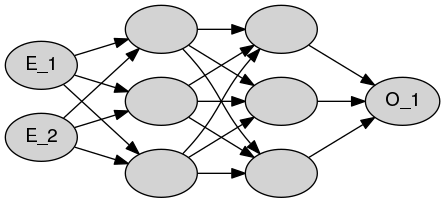
\includegraphics[width=0.6\linewidth]{Bilder/netz.png}
\end{center}
\begin{itemize}
	\item Verfahren des maschinellen Lernens
	\item Zur Regressionsanalyse verwendet
	%Bestimmung der Zusammenhänge der Attribute des Eingabevektors zu den Attributen des Ausgabevektors
	%Bild einfaches feedforward-Netz, eingabevektor mit 2 attributen, ausgabevektor mit einem, und 2 verdeckten schichten
		\begin{itemize}
			\item Überwachtes Lernen
			%Vorgabe von Ausgabewerten als Lösungen
			%\item Trainingsdatensatz
			%Beim Lernvorgang verwendete Daten
			%\item Testdatensatz
			%ungesehene Daten zur Überprüfung der Abstraktionsfähigkeit des Modells
		\end{itemize}
	\item Trainieren durch Fehlerrückführung
	%mittlere quadratische Fehler gegenüber idealer Ausgabe berechnen und mit Gradientenverfahren Gewichtsupdate berechnen
	\item Mächtiger als lineare Regression
	%Mit ausreichender Komplexität des Netzes Approximation beliebiger kontinuierlicher Funktionen
	%universal approximation theorem von Cybenko
\end{itemize}

\column{.43\textwidth}
\begin{figure}
	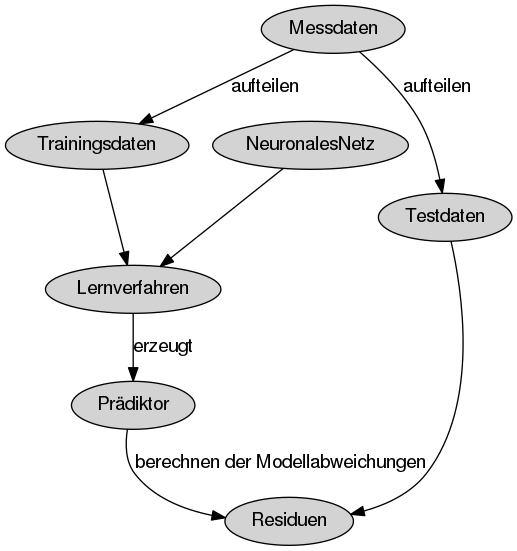
\includegraphics[width=1.1\linewidth]{Dot/tupel1.png}
	%\vspace*{0.5cm}
	%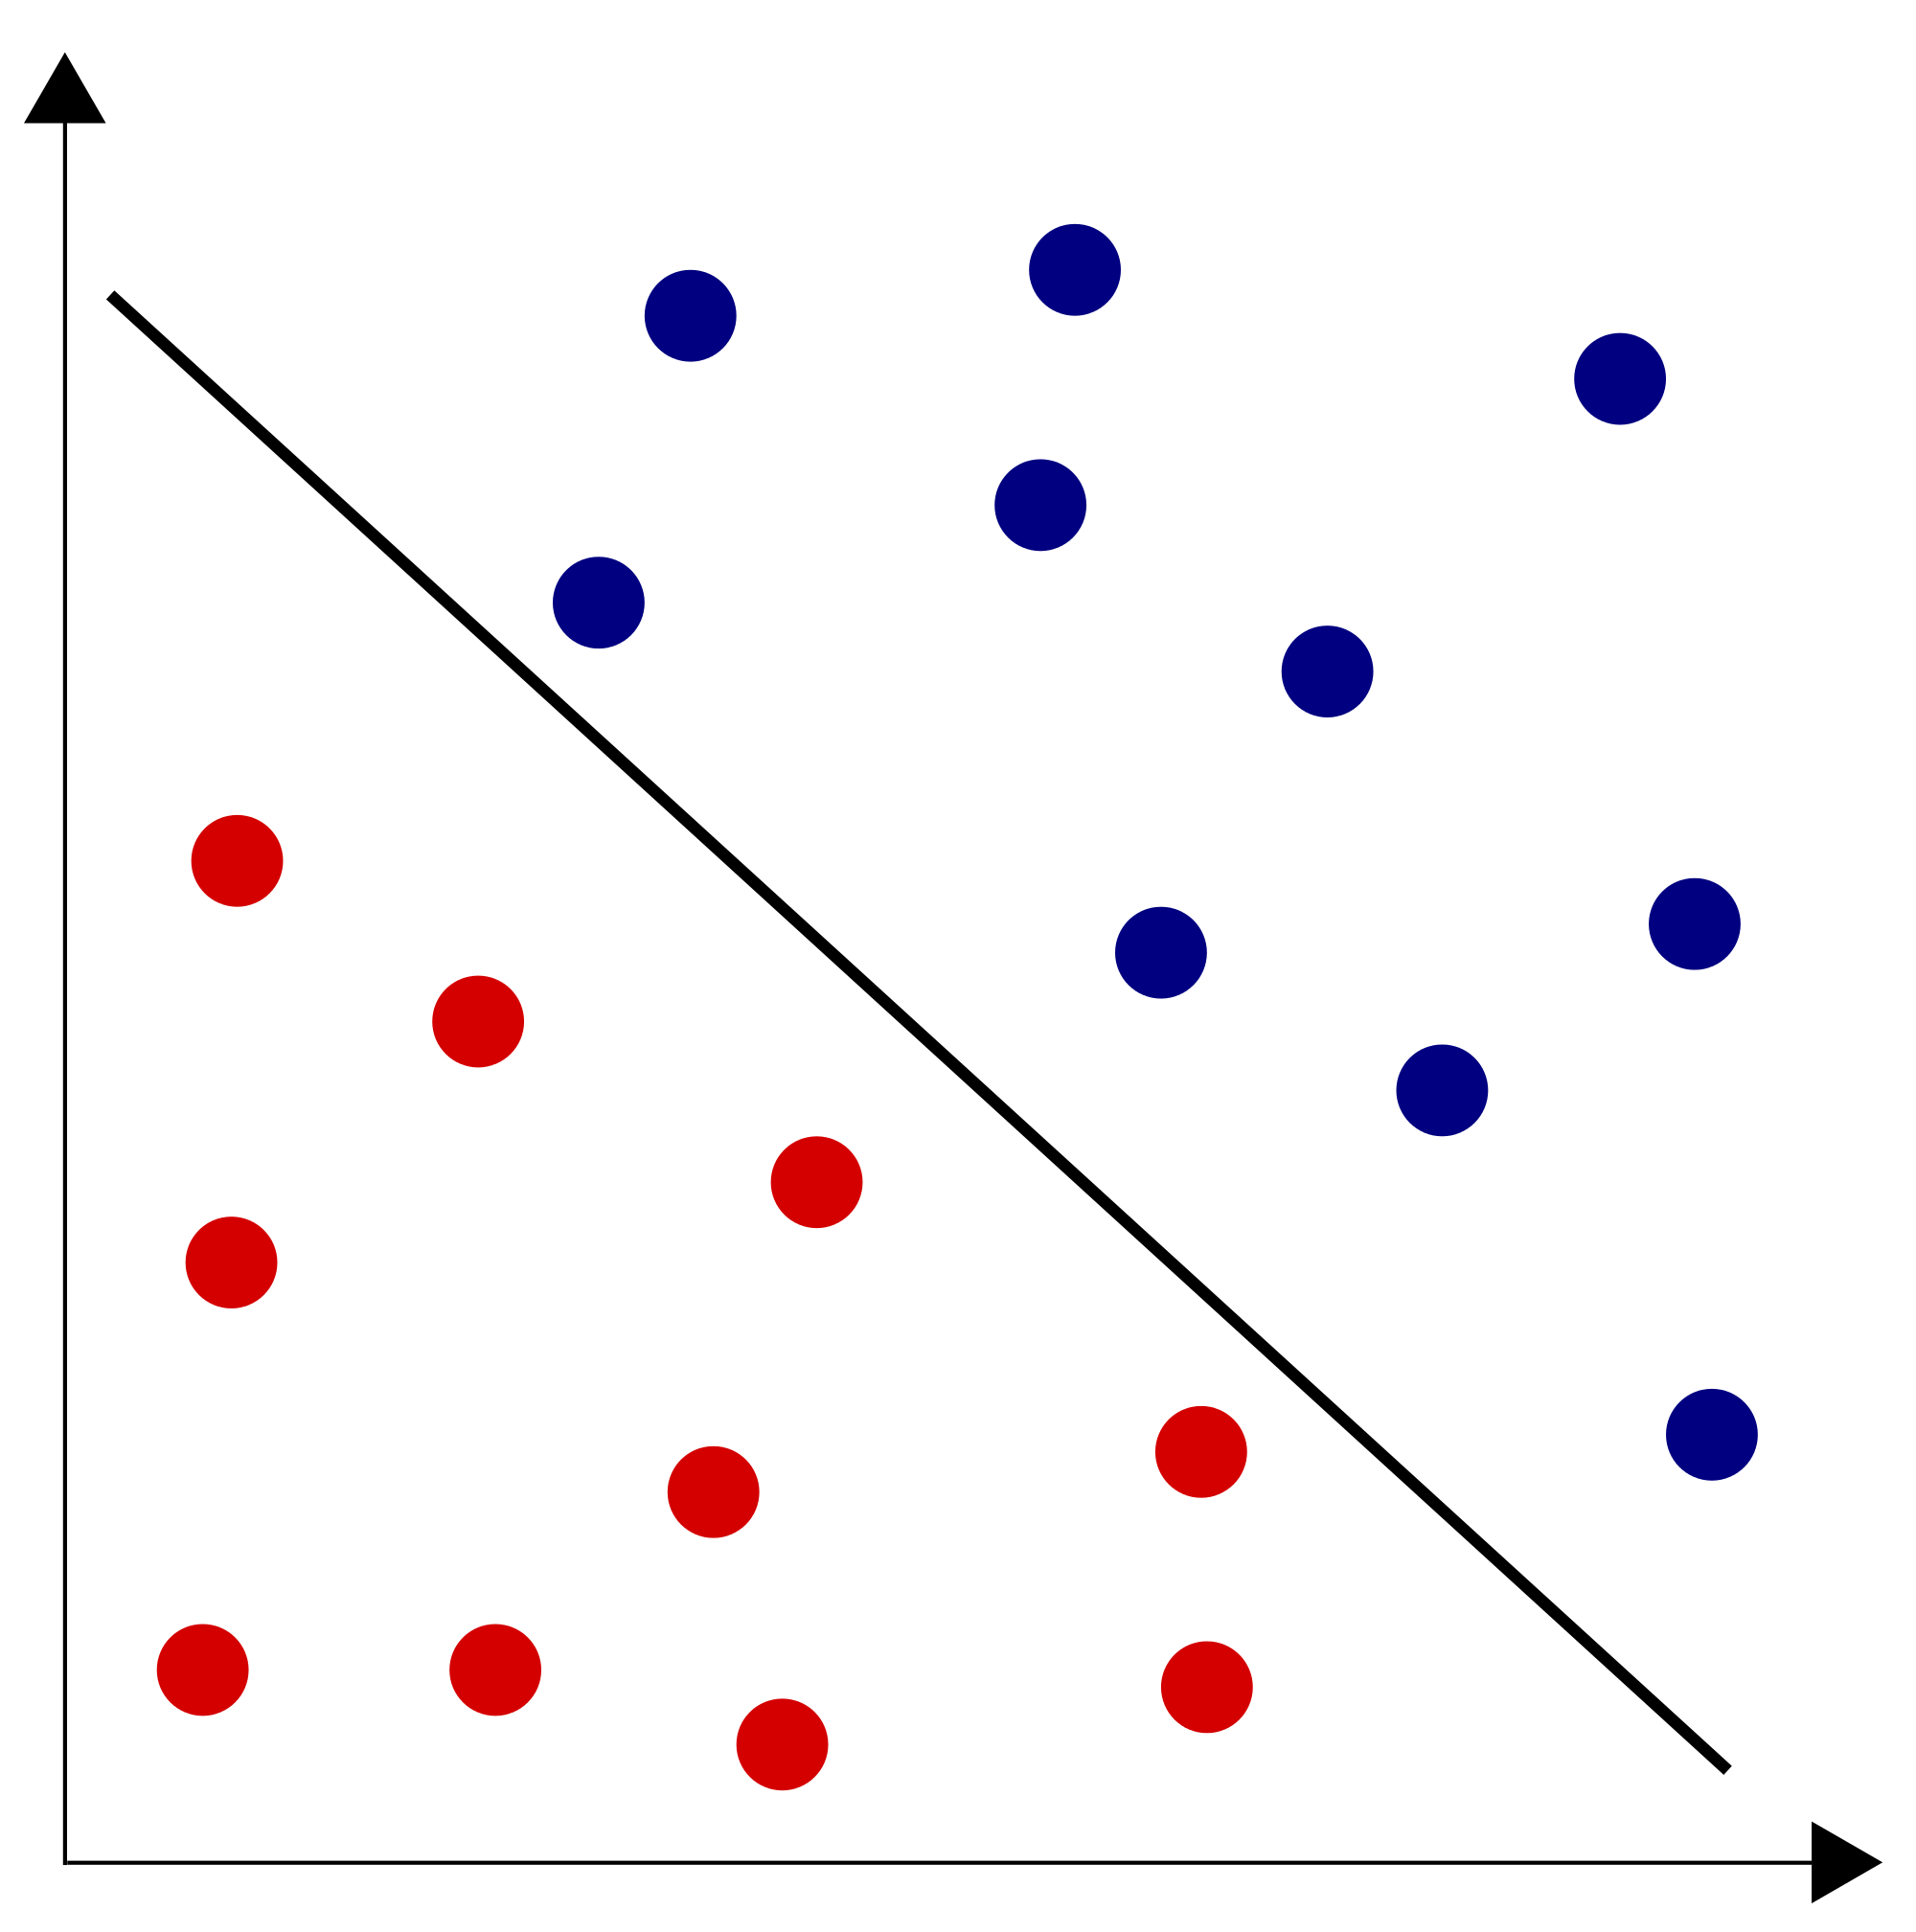
\includegraphics[width=0.45\linewidth]{Bilder/2000px-Separability_YES.png}\ %footnotemark
	%\hspace*{0.3cm}
	%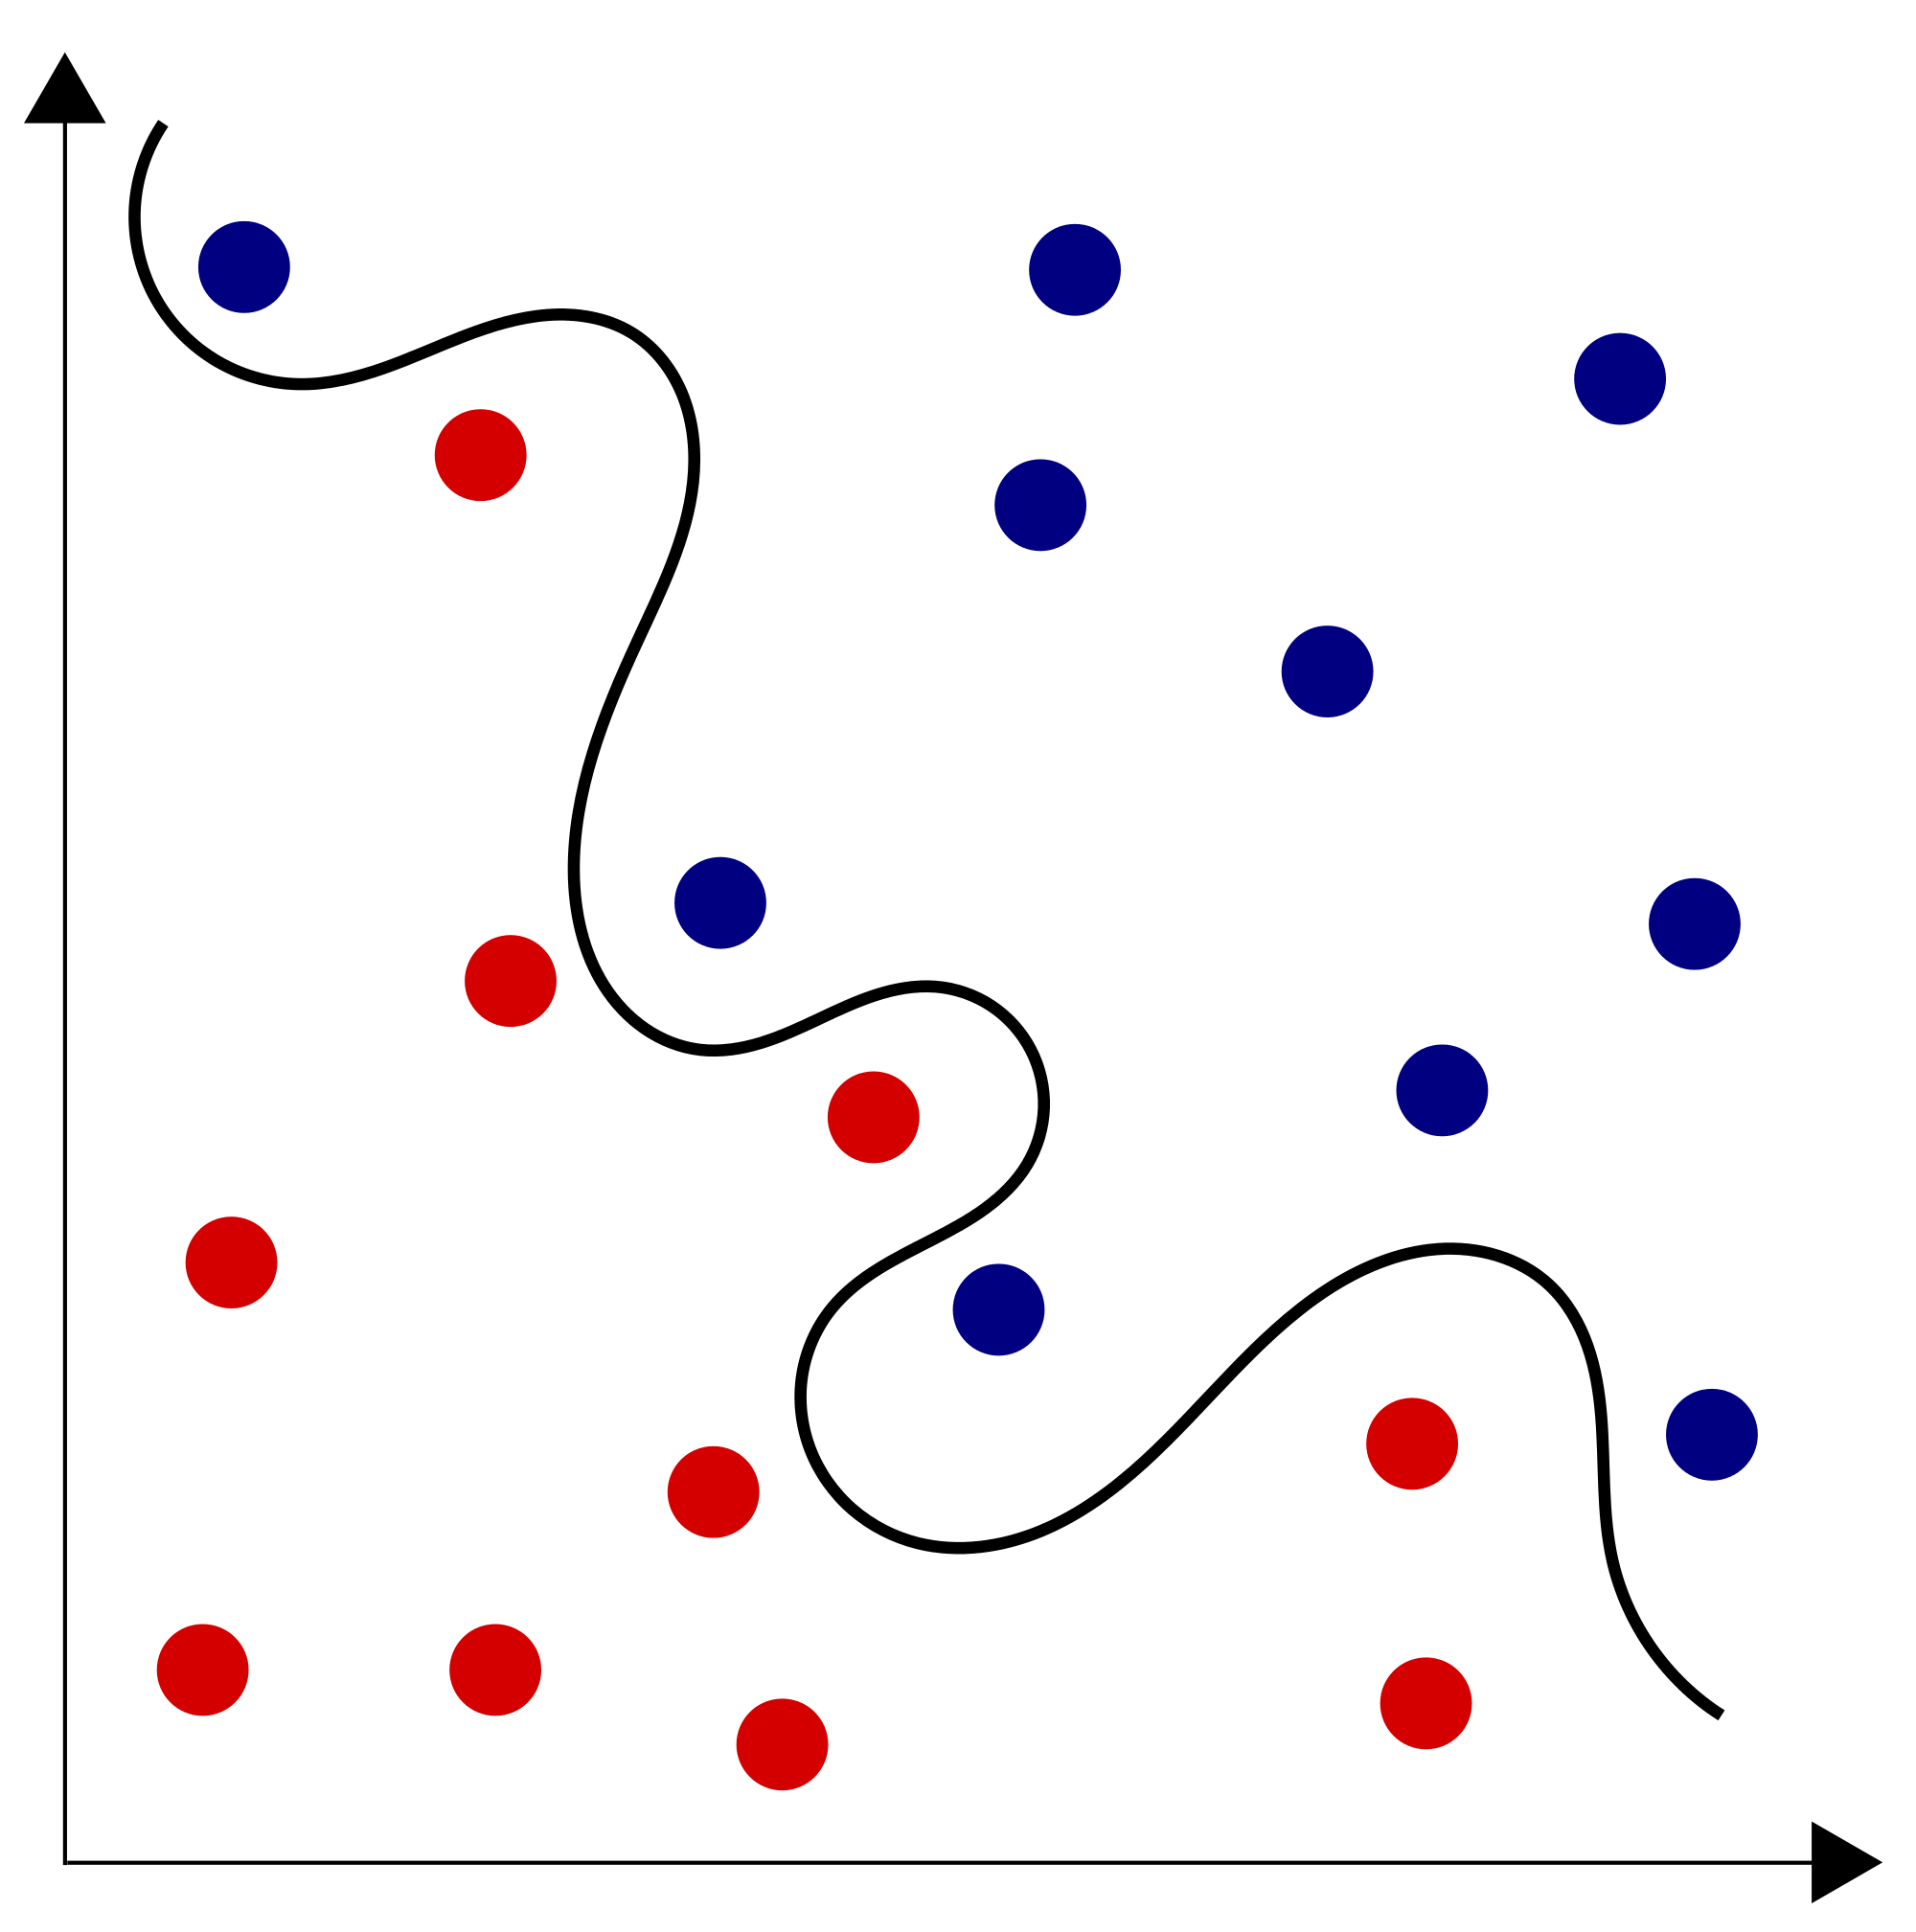
\includegraphics[width=0.45\linewidth]{Bilder/2000px-Separability_NO.png}
\end{figure}
\end{columns}
\end{frame}

\section{Modell des Ein-/Ausgabe-Pfads}
%speicherhierachie, Zugriffszeit davon abhängig
\begin{frame}
\frametitle{Modell des Ein-/Ausgabe-Pfads}
\begin{columns}
\column{.6\textwidth}
\begin{itemize}
	%\item<1-> Modell des E/A-Systems
	%Unterscheidung von drei Anteilen des Zeitaufwandes zum Bearbeiten einer Anfrage: Festplatten, Netzwerk, Arbeitsspeicher+Caches
	\item<1-> Verarbeitung eines Zugriffs entlang des E/A-Pfades
	%Pfad abhängig davon wo Daten sich befinden
	%Zeitanteil in den drei Bereichen hängt vom Durchsatz und Latenzen ab
	\item<1-> Zugriffszeit wesentlich durch tiefe des Pfades bestimmt
	%durch Speicherhirachie hängt Verarbeitungszeit von der langsamsten Komponente ab
	%\item<1-> Speicherhierachie
	 %System entspricht einer Hierachie von verschiedenen Speichermedien
\end{itemize}

\column{.5\textwidth}
\begin{figure}
	\vspace*{-1cm}
	\includegraphics<1>[width=0.95\linewidth]{Bilder/rechnerknoten.png}
	\includegraphics<2->[width=0.95\linewidth]{Bilder/rechnerknoten_ea_pfad.png}
	\vspace*{+0.4cm}
	\hspace*{-1cm}
	\uncover<3->{\includegraphics<1->[width=1.25\linewidth]{Bilder/hierachie.png}}
\end{figure}
\end{columns}
\end{frame}

\section{Evaluierung}
\subsection{Benchmark-Tests}
%welche Messreihen wurden gemacht, auf welchem Rechner, welche Daten stehen zur Verfügung, wie sehen daten aus?
\begin{frame}
\frametitle{Attribute der Messdaten}
%System wird mit Messungen untersucht, beschränktes Wissen dabei:
%\begin{columns}
%	\column{.7\textwidth}
\vspace*{0.13cm}
	\begin{itemize}
		\item Parameter eines E/A-Aufrufs:
		\begin{itemize}
			\item Datei ID
			%zur Identifikation der aufgerufenen Datei
			\item \textbf{Zugriffsgröße}
			%Anazahl Bytes die gelesen/geschrieben werden sollen
			\item Offset
			%Abstand vom Dateibeginn bis zum zugegriffenen Bereich
			\item \textbf{Delta-Offset} %$\text{Offset}[i]-(\text{Offset}[i-1]+\text{Zugriffsgröße}[i-1])$
			%Strecke die Dateizeiger zurücklegen muss			
			\item \textbf{Operationstyp} 
			%lesend oder schreibend
		\end{itemize}
		\item Messbare Größen:
			\begin{itemize}
				\item Zeitpunkt der Anfrage
				\item \textbf{Zugriffszeit}
			\end{itemize}
		\item Keine Informationen über den E/A-Pfad
		%weder vor dem Aufruf bekannt noch dabei/danach direkt messbar
		%gecached oder nech?
	\end{itemize}
%	\column{.5\textwidth}
		\begin{figure}
			\includegraphics<1>[width=0.781\linewidth]{Bilder/deltaoffset.png}
		\end{figure}
%\end{columns}
\end{frame}

\begin{frame}
\frametitle{Benchmark-Tests}
%Messreihen und Testsystem
\begin{itemize}
	\item Zwei untersuchte Anwendungsfälle:
	\begin{itemize}
		\item \textbf{SEQ:} Sequentieller Zugriff auf hintereinanderliegende Daten
		\item \textbf{RND:} Zufälliger Zugriffsort 
	\end{itemize}
	\item Zugriffsgrößen von 1\,B bis 16\,MiB
	\item Jeweils lesende und schreibende Messreihen
	
	%3 Messreihen mit 10.000 Messungen pro Anwendungsfall und Zugriffsart, 
\end{itemize}
	\begin{block}{Hardwarekonfiguration des Testsystems Mistral}
	\begin{itemize} 
		\item Über 1500 Knoten
		\item 30 Petabyte Speicherkapazität
		\item Speichersystem Lustre
	\end{itemize}
\end{block}
\end{frame}

\subsection{Exploration der Messdaten}
\begin{frame}
\frametitle{Messungen sortiert nach Zugriffsgröße}
\begin{columns}
\column{.45\textwidth}
	\begin{figure}
		\includegraphics<1->[width=1\linewidth]{Bilder/plot_SizeSorted_log_read_seq.png}\\
		\vspace*{-0.45cm}
		\caption{SEQ lesend}
		\uncover<2->{\includegraphics<1->[width=1\linewidth]{Bilder/plot_SizeSorted_log_read_rnd.png}
			\vspace*{-0.45cm}
			\caption{RND lesend}}	
	\end{figure}
\column{.45\textwidth}
	\begin{figure}
		\uncover<2->{\includegraphics<1->[width=1\linewidth]{Bilder/plot_SizeSorted_log_write_seq.png}
		\\
		\vspace*{-0.45cm}
		\caption{SEQ schreibend}}
		\uncover<2->{\includegraphics<1->[width=1\linewidth]{Bilder/plot_SizeSorted_log_write_rnd.png}
		\vspace*{-0.45cm}
		\caption{RND schreibend}}
	\end{figure}
	%jede Farbe eine Messgröße, im Seq Fall komplett gleiche Attribute
	%1 B, 4 B, 16 B, 64 B, 256 B, 1 KiB, 4 KiB,8 KiB, 16 KiB, 64 KiB, 256 KiB,512 KiB, 1 MiB, 2 MiB, 4 MiB,8 MiB und 16 MiB
	%Betrachtung in Zeitreihe
	%3 Messreihen direkt hintereinader
	%Starke Abhängigkeit von Zugriffsgröße erkennbar, aber muss mehr geben (RND-R)
	%deutlich zu erkennen, dass Messungen mit gleichen Attributen zu sehr unterschiedlichen ergebnissen führen können
	%Aufteilung der Messungen mit selben Attributen in über mehrere Zugriffsgrößen übergreifende Gruppen, keine gleichmäßige Verteilung wie zu erwarten wäre -> E/A-Pfad
	%Zugriffszeit stärker vom E/A-Pfad als von Zugriffsgröße abhängig
	%Es ist notwendig(!) innerhalb der Menge von Messungen mit gleichen Attributen zu unterscheiden, wenn sehr gute Vorhersagen gemacht werden sollen
\end{columns}
\end{frame}

%\begin{frame}
%zeigen, warum Betrachtung der zeitlichen Periodizität durchaus legitim ist
%\frametitle{Detailbetrachtung: Messungen mit 16\,KiB}
%\begin{columns}
%\column{.6\textwidth}
%\begin{itemize}
%	%16KiB lesende Zugriffe
%	\item Lesende Zugriffe von 16\,KiB
%	\item Sich wiederholende Muster (Periodizität)
%	\item Abhängigkeit von der Messreihe
%\end{itemize}
%\column{.45\textwidth}
%	\begin{figure}
%		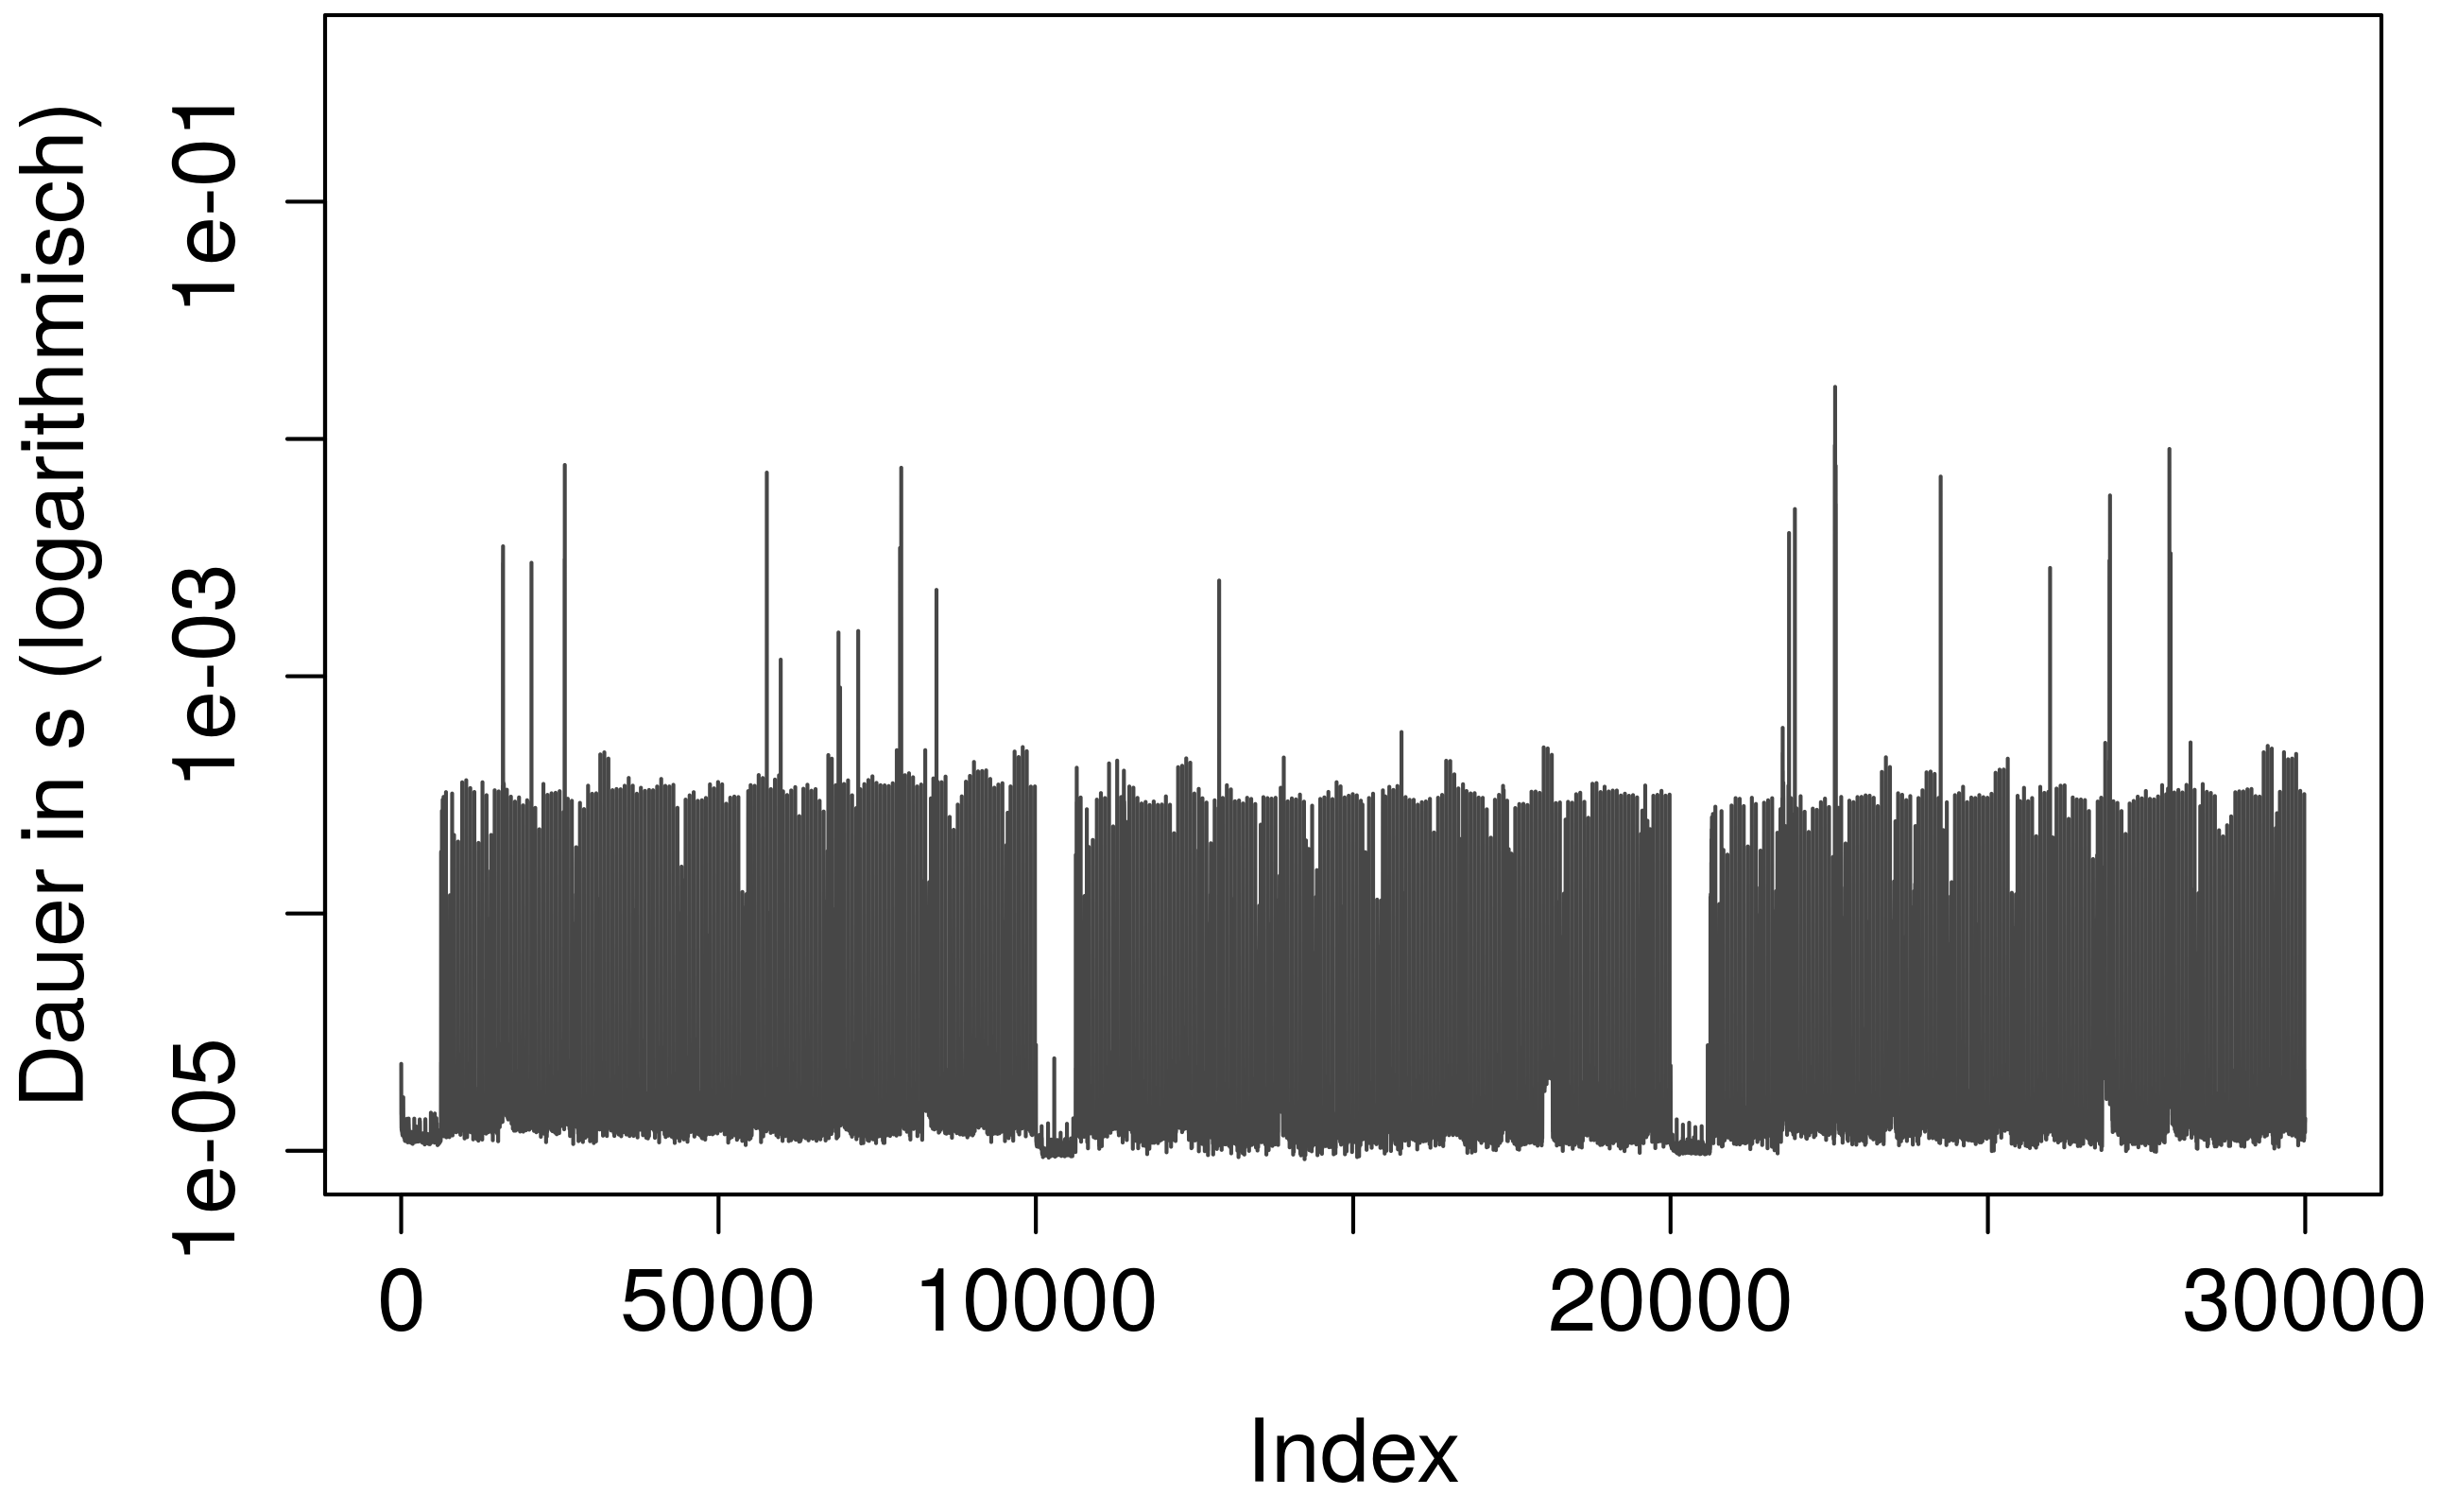
\includegraphics[width=1\linewidth]{Bilder/plot_Size16384_read_seq.png}\\
%		\vspace*{-0.45cm}
%		\caption{SEQ lesend}
%		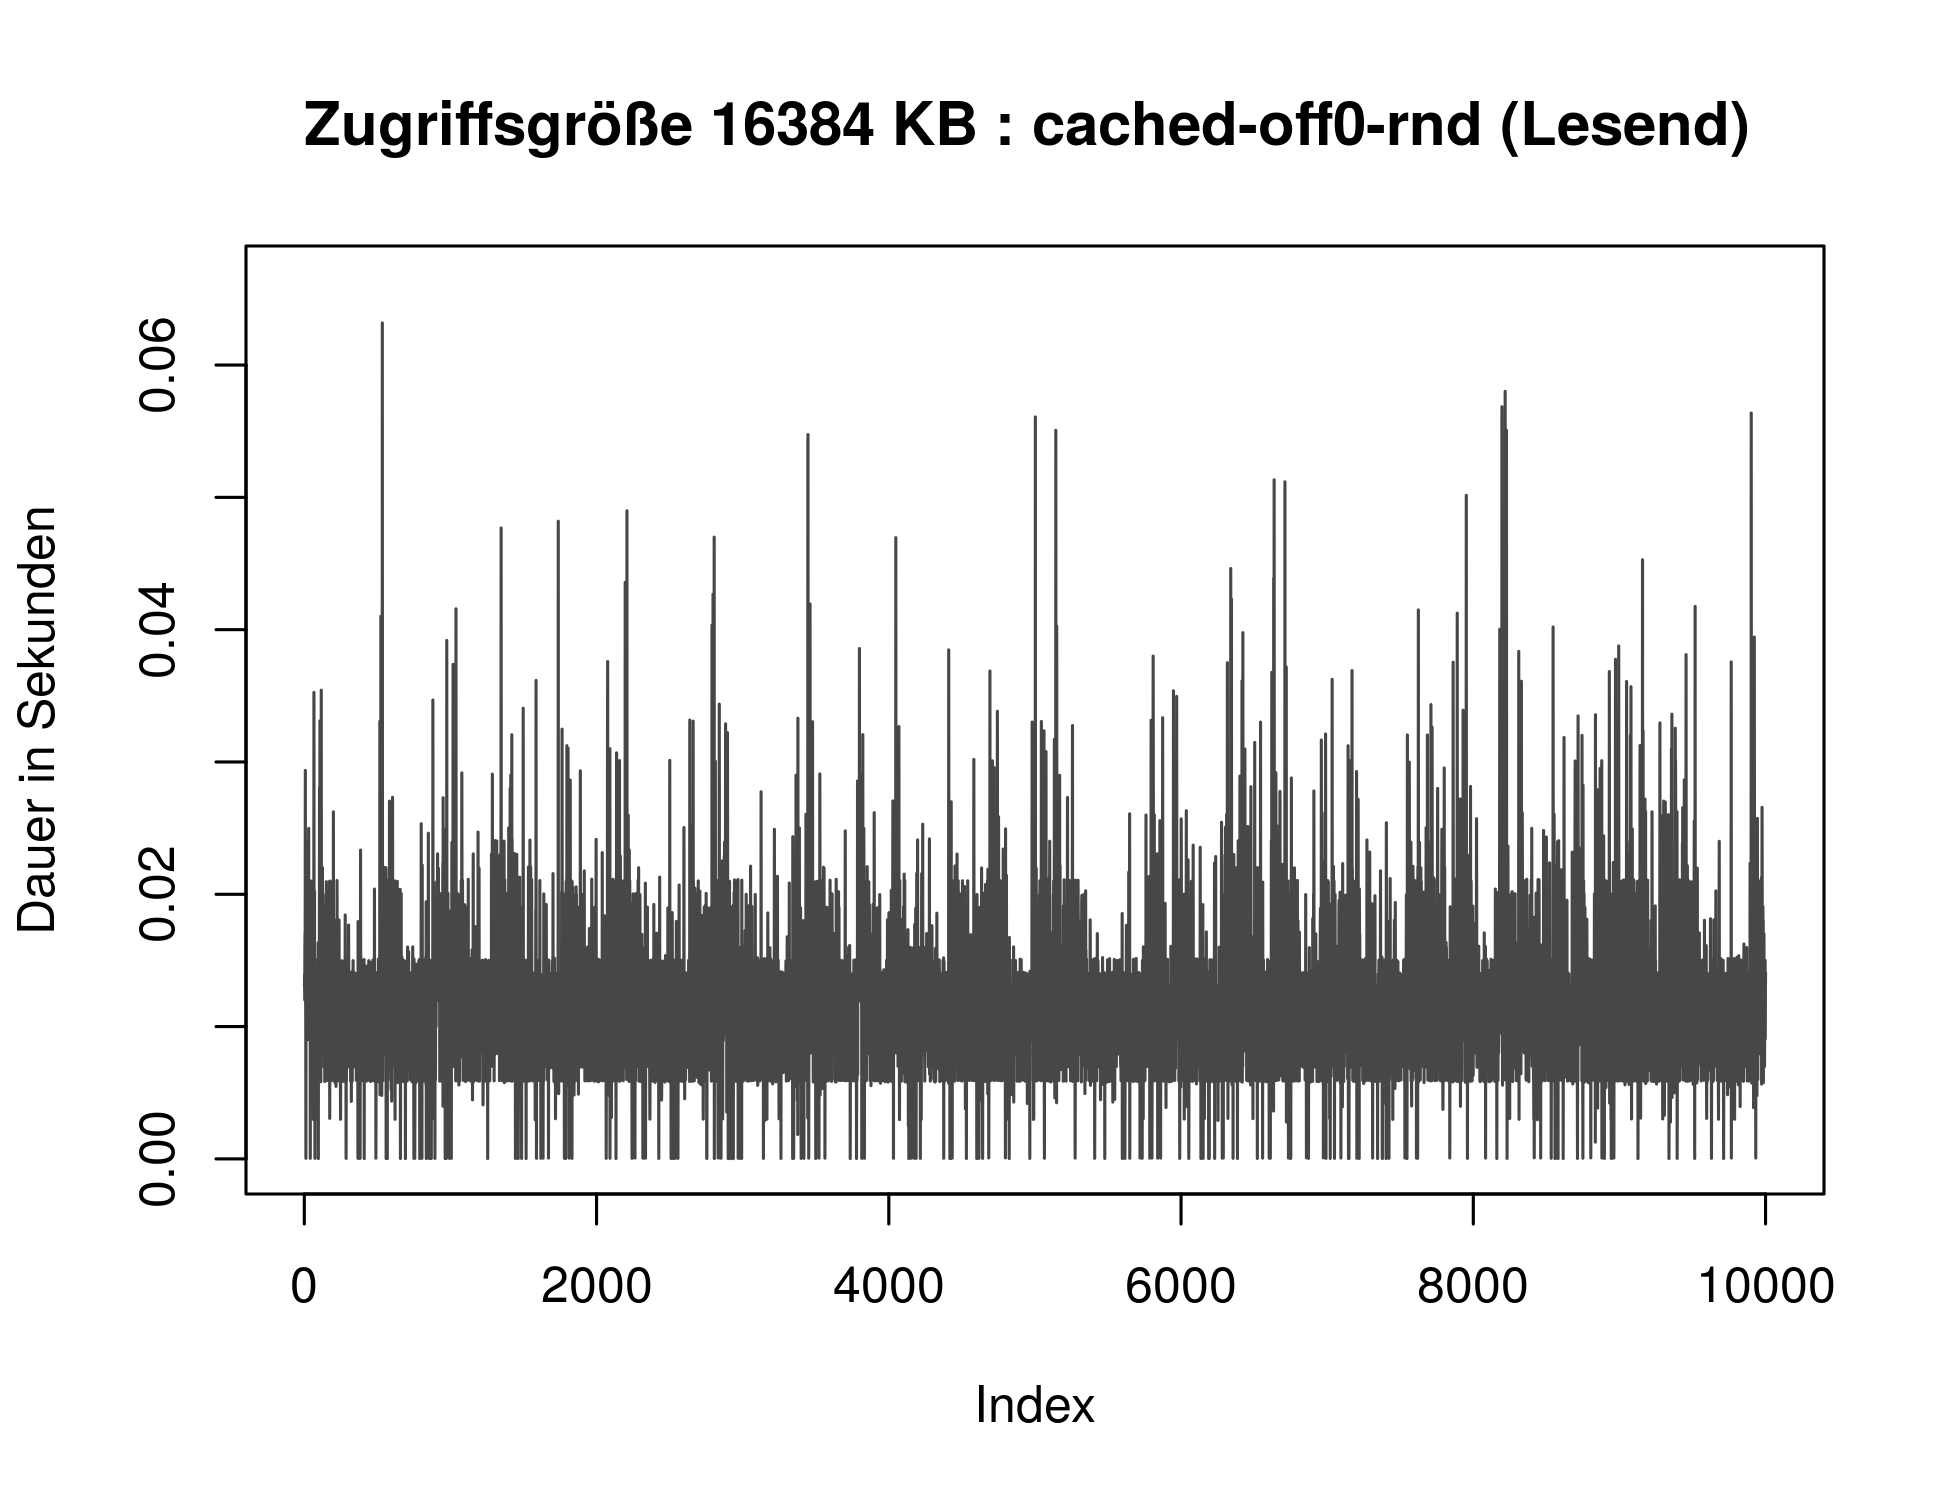
\includegraphics[width=1\linewidth]{Bilder/plot_Size16384_read_rnd.png}
%		\vspace*{-0.45cm}
%		\caption{RND lesend}
%	\end{figure}
%\end{columns}
%\end{frame}

\begin{frame}
%zeigen, warum Betrachtung der zeitlichen Periodizität durchaus legitim ist
\frametitle{Detailbetrachtung: 250 Messungen auf SEQ}
\begin{columns}
\column{.45\textwidth}
	\begin{figure}
		\includegraphics<1->[width=1\linewidth]{Bilder/plot_First250_read_seq.png}\\
		\vspace*{-0.45cm}
		\caption{SEQ lesend}
		\includegraphics<1>[width=1\linewidth]{Bilder/plot_First250_write_seq.png}
		\includegraphics<2->[width=1\linewidth]{Bilder/plot_periodicitywrite_seq.png}
		\vspace*{-0.45cm}
		\caption{SEQ schreibend}
	\end{figure}
\column{.45\textwidth}
	\begin{figure}
		\includegraphics<1>[width=1\linewidth]{Bilder/plot_From100001to100250_read_seq.png}
		\includegraphics<2->[width=1\linewidth]{Bilder/plot_periodicity100001read_seq.png}
		\\
		\vspace*{-0.45cm}
		\caption{SEQ lesend}
		\includegraphics<1->[width=1\linewidth]{Bilder/plot_From100001to100250_write_seq.png}
		\vspace*{-0.45cm}
		\caption{SEQ schreibend}
	\end{figure}
\end{columns}
\end{frame}

\section{Modelle zur Leistungsvorhersage}
%lineare vs nn modelle und ema modell, was sind die Modelle überhaupt?
\begin{frame}
\frametitle{Modelle zur Leistungsvorhersage}
\begin{columns}
	\column{.55\textwidth}
\begin{itemize}
	\item<1-> Durchschnittliche Zugriffszeit (\textbf{Durchschnitt})
	\item<2-> Lineare Regression nach der Zugriffsgröße (\textbf{LinReg G})
	%nach weiteren Attributen als nicht besser herausgestellt
	\item<3-> Einfaches Modell mit neuronalem Netz (\textbf{NN-Tupel1})
	%Zugriffsgröße, DeltaOffset, OpTyp auf Zugriffszeit
	\item<4-> Ausnutzen zeitlicher Abhängigkeit mit dem \textit{exponential moving average}(\textbf{NN-EMA})
	%ema, exponential moving average
	%2 BILDER erstellen! einmal attribute zu zugriffsdauer und einmal beispiel von ema
\end{itemize}
	\column{.6\textwidth}
	\begin{figure}
		\includegraphics<2>[width=0.95\linewidth]{Dot/linreg.png}
		\includegraphics<3>[width=0.95\linewidth]{Dot/nntupel1.png}
		\uncover<4>{\includegraphics[width=0.95\linewidth]{Dot/ema.png}\\
			\vspace*{+1cm}
			\hspace*{-0.45cm}
		\includegraphics[width=1.05\linewidth]{Bilder/ema.png}}
	\end{figure}
\end{columns}
\end{frame}

\subsection{Ergebnisse}
\begin{frame}
	\frametitle{Modelle angewendet auf SEQ}
	\begin{columns}
		\column{.45\textwidth}
		\begin{figure}
			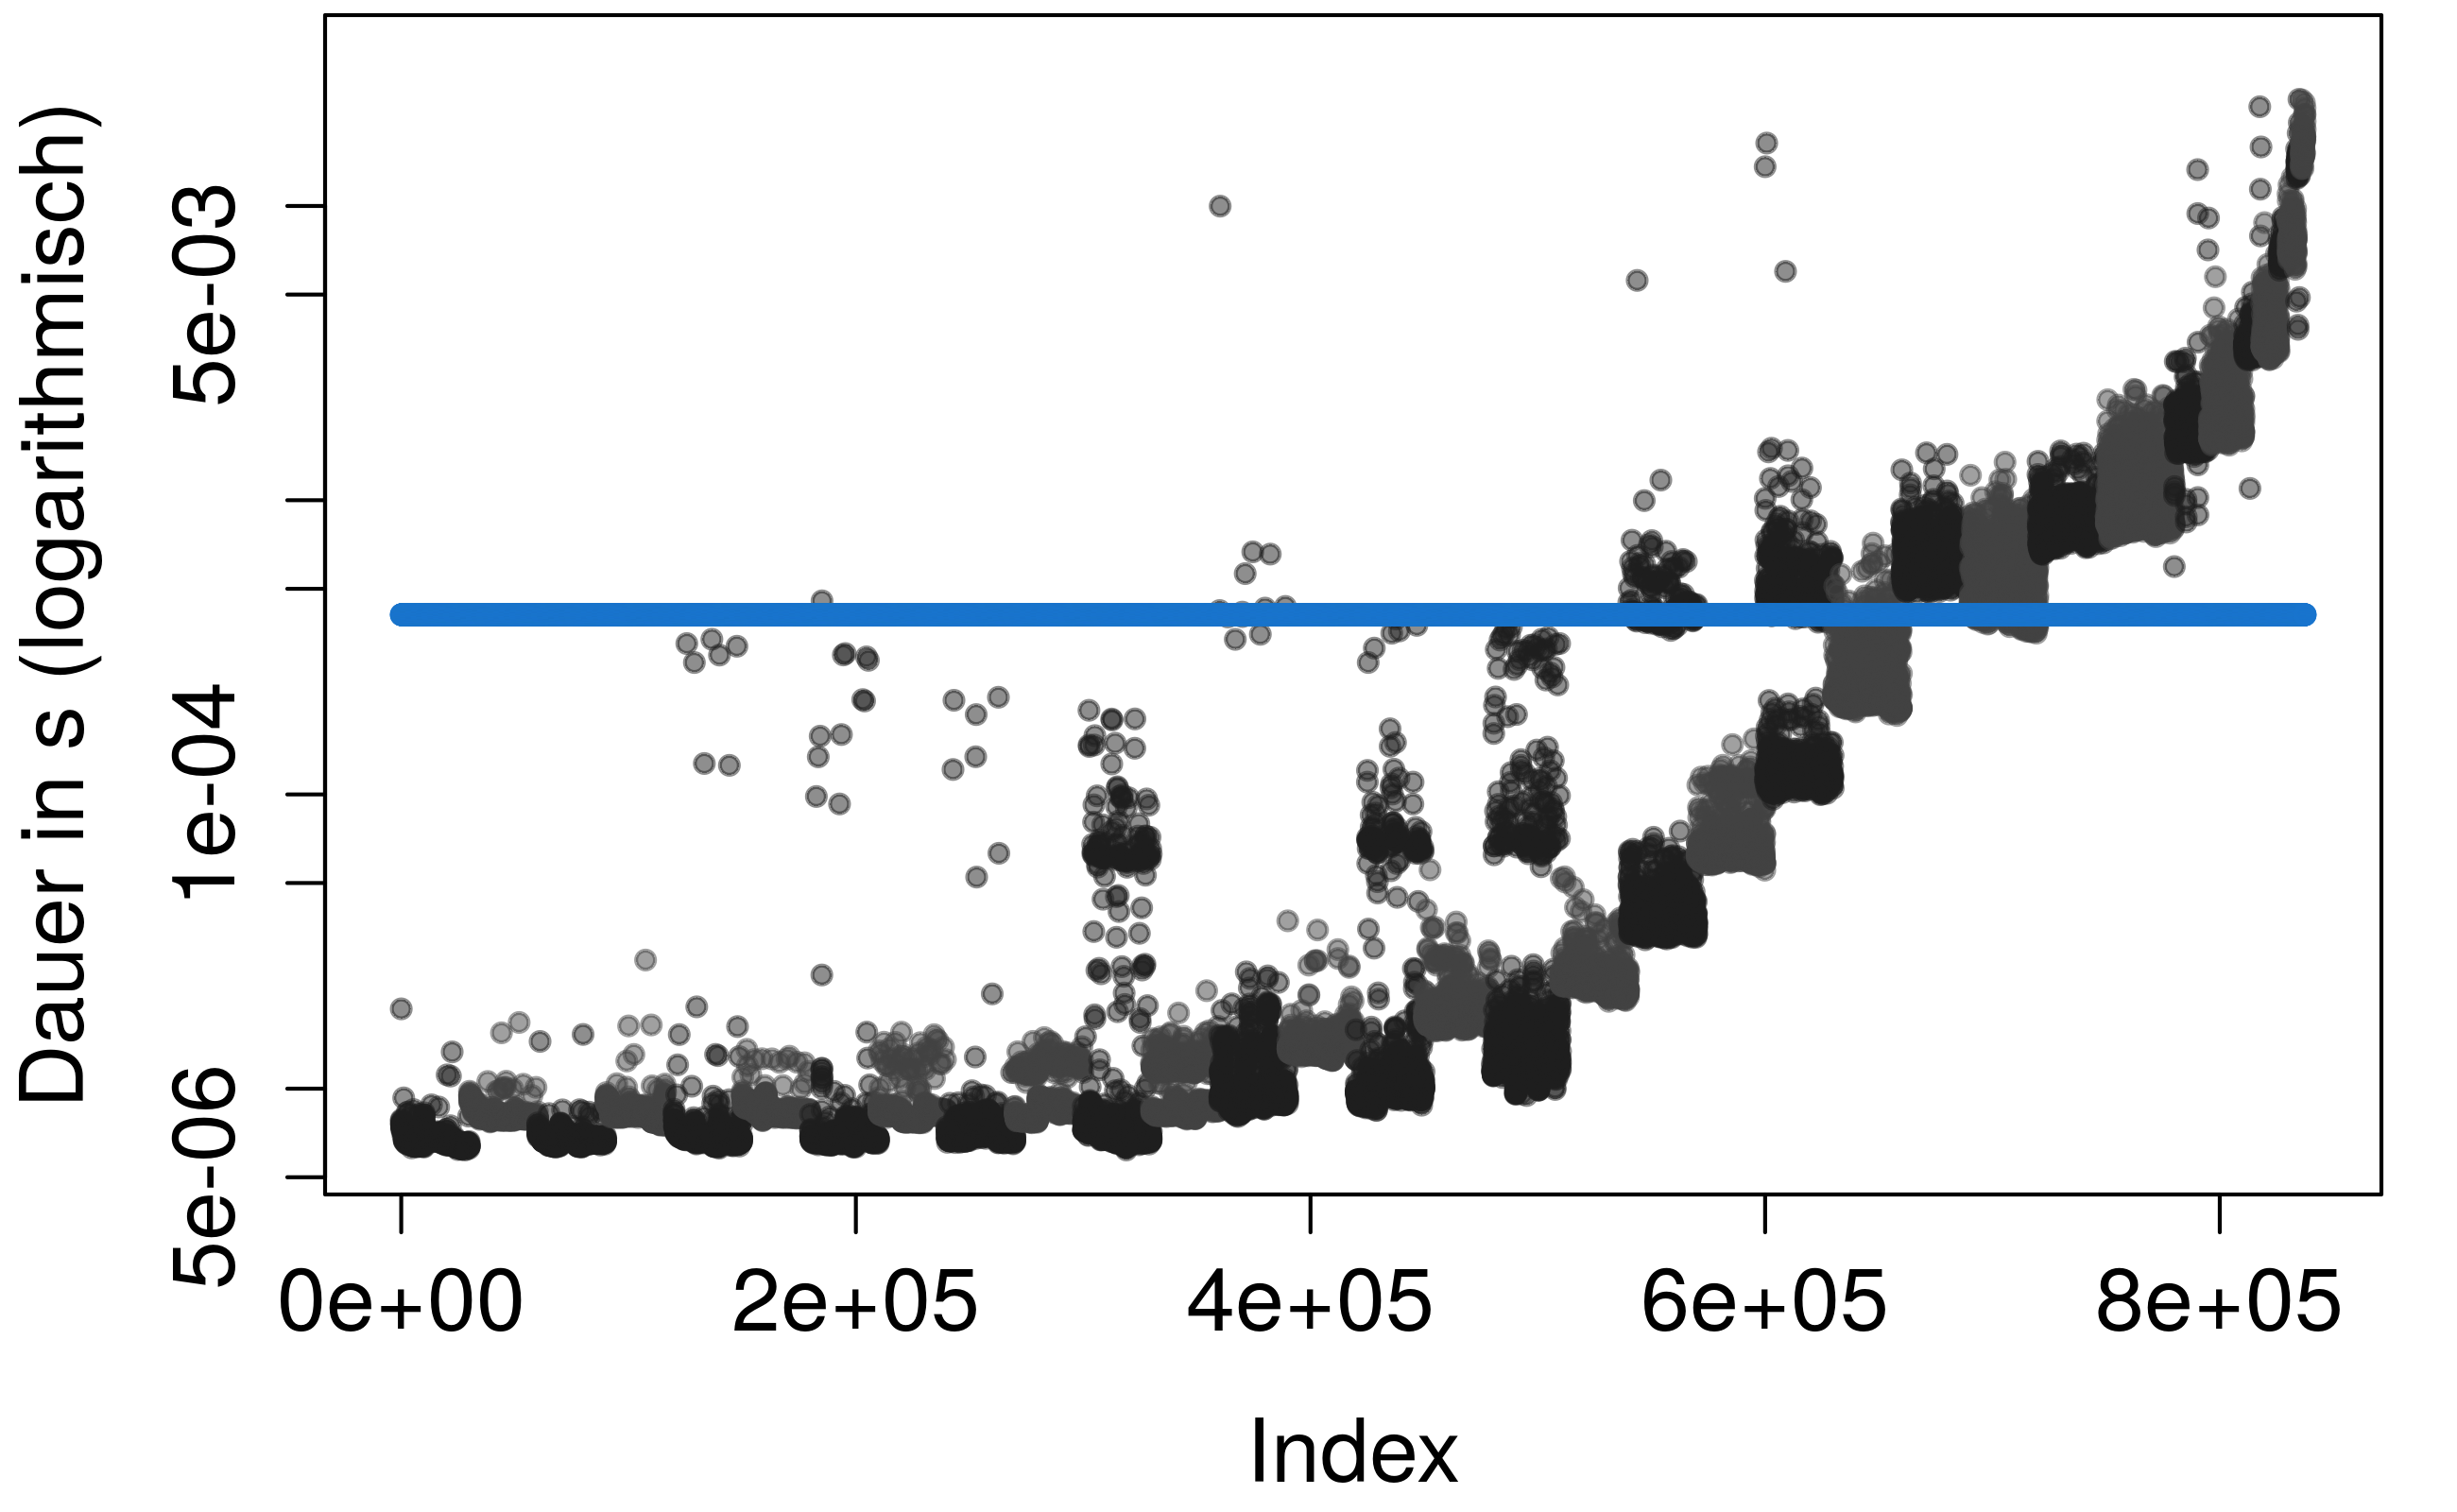
\includegraphics[width=1\linewidth]{Bilder/plot_seq_mean_performance.png}\\
			\vspace*{-0.45cm}
			\caption{Durchschnitt}
			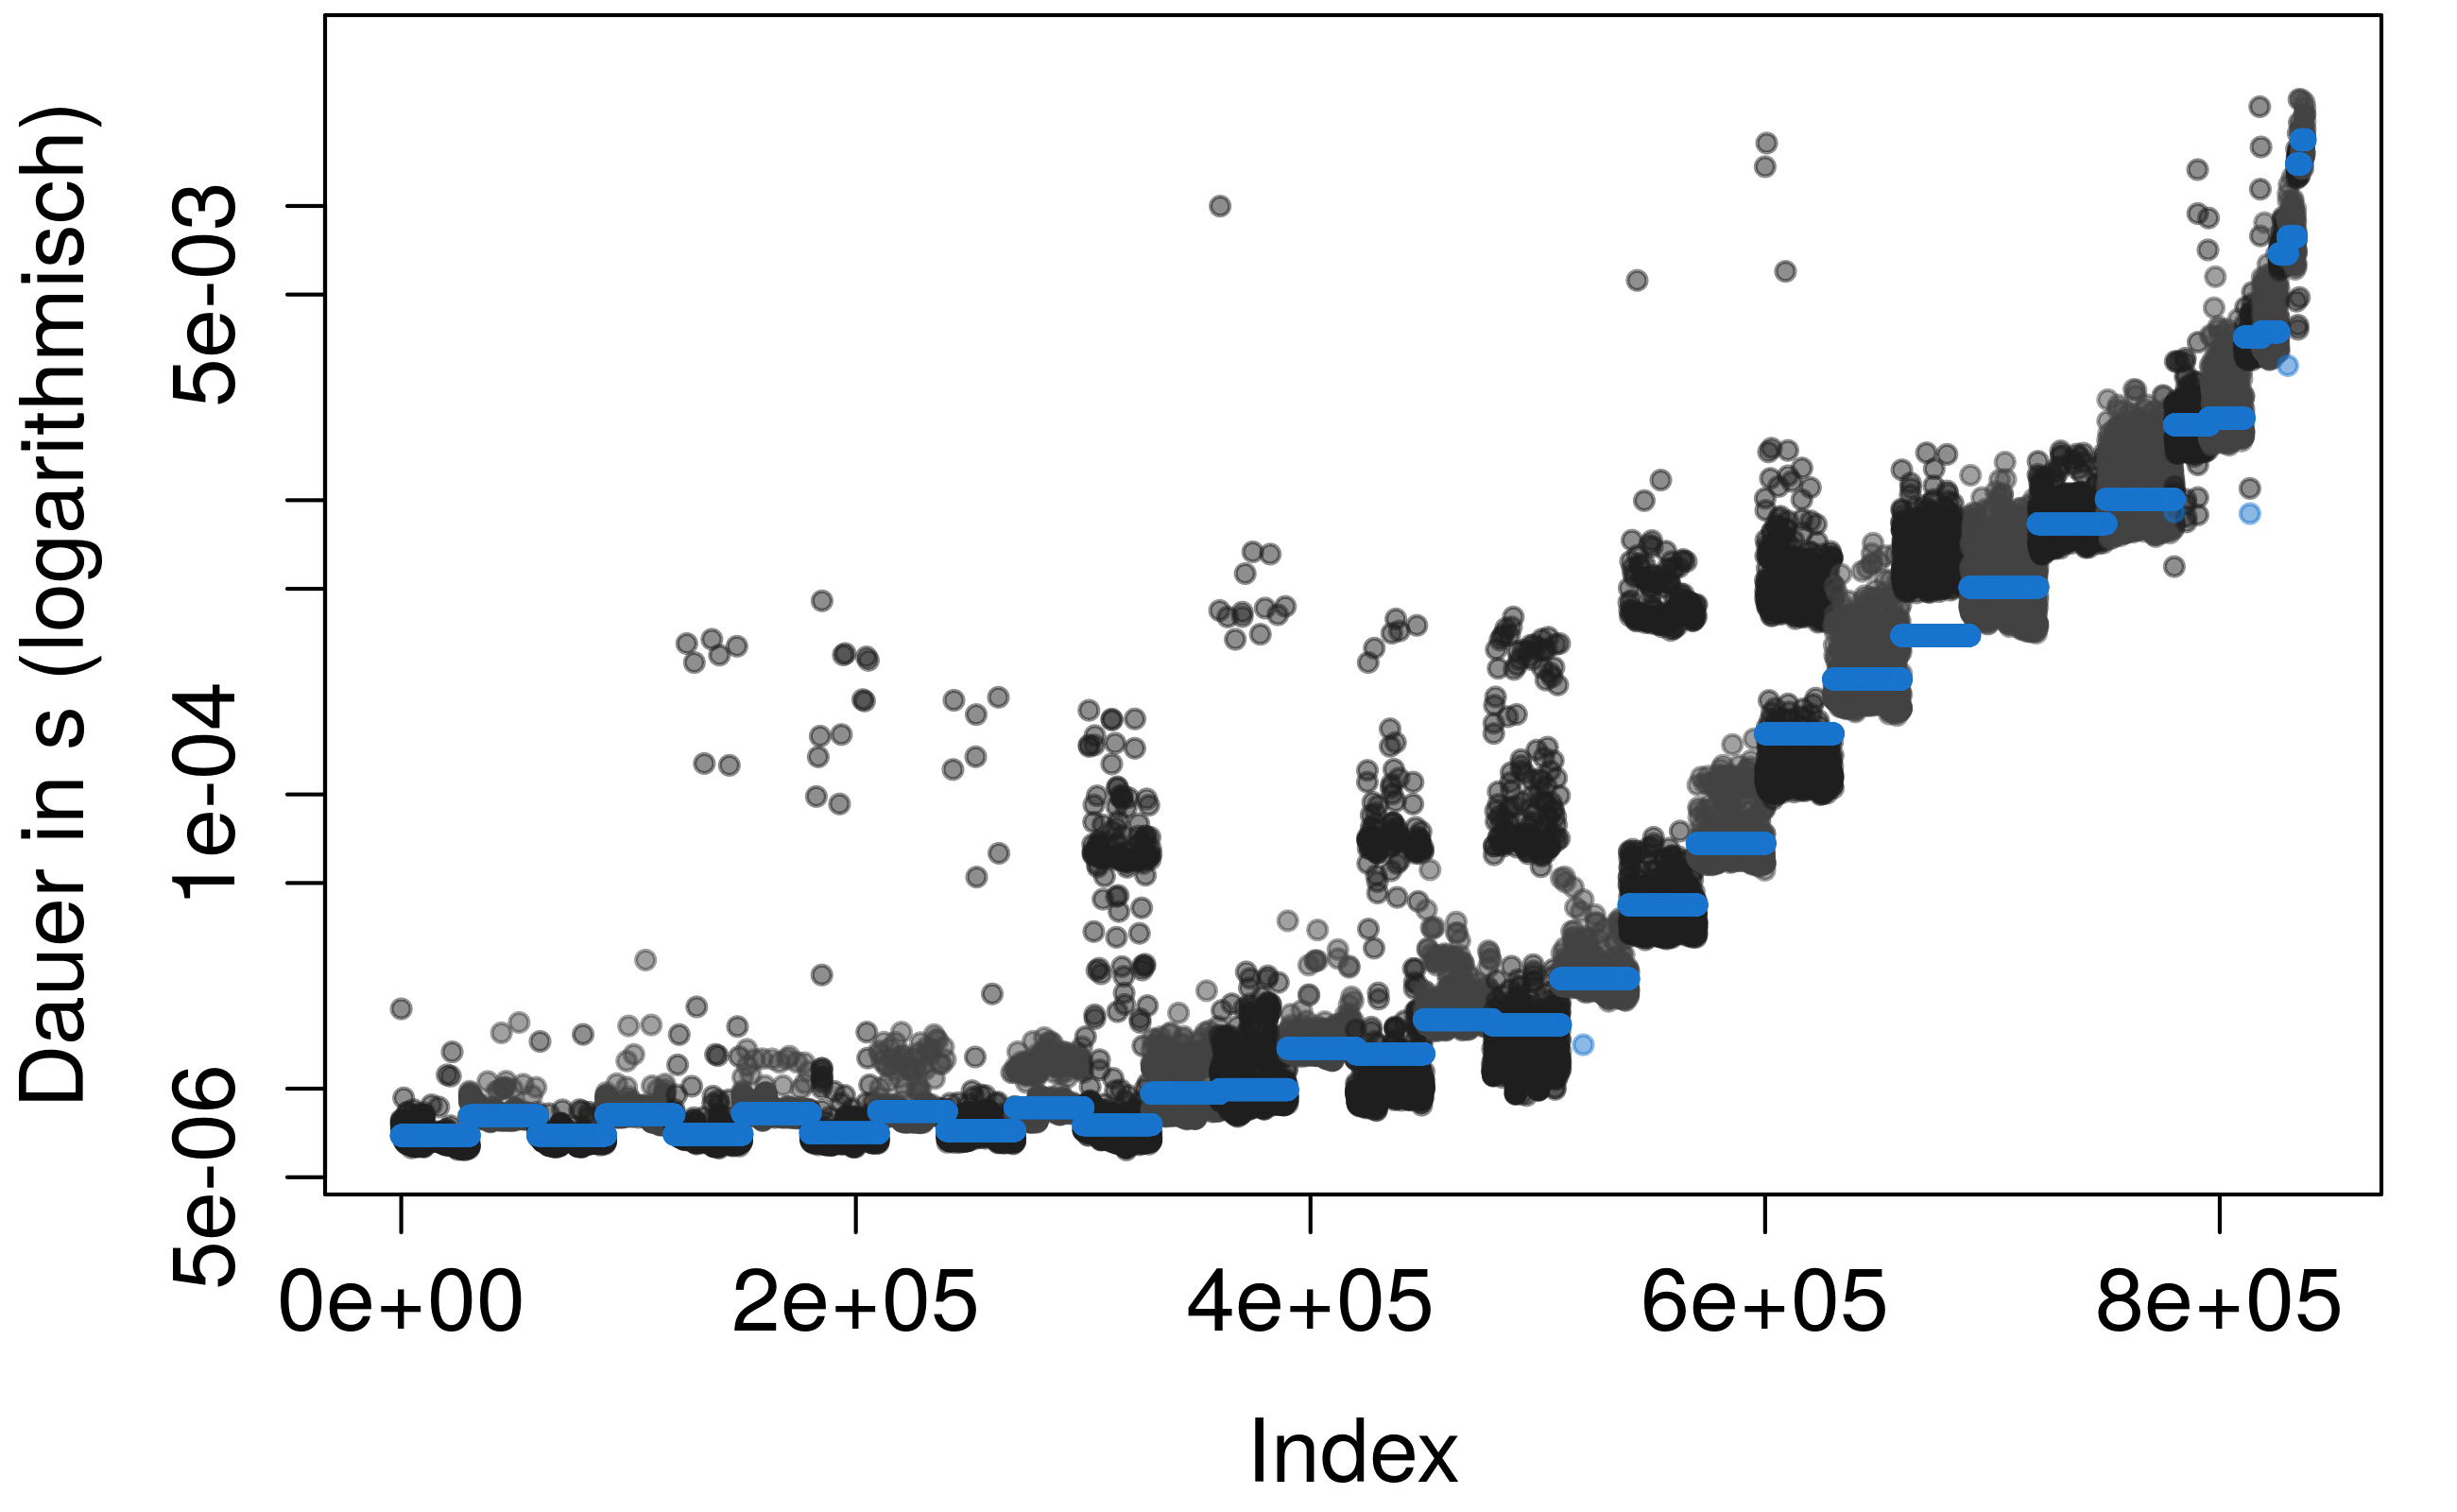
\includegraphics[width=1\linewidth]{Bilder/plot_onlyPred_tuple1_Duration_seq.png}
			\vspace*{-0.45cm}
			\caption{NN-Tupel1}
		\end{figure}
		\column{.45\textwidth}
		\begin{figure}
			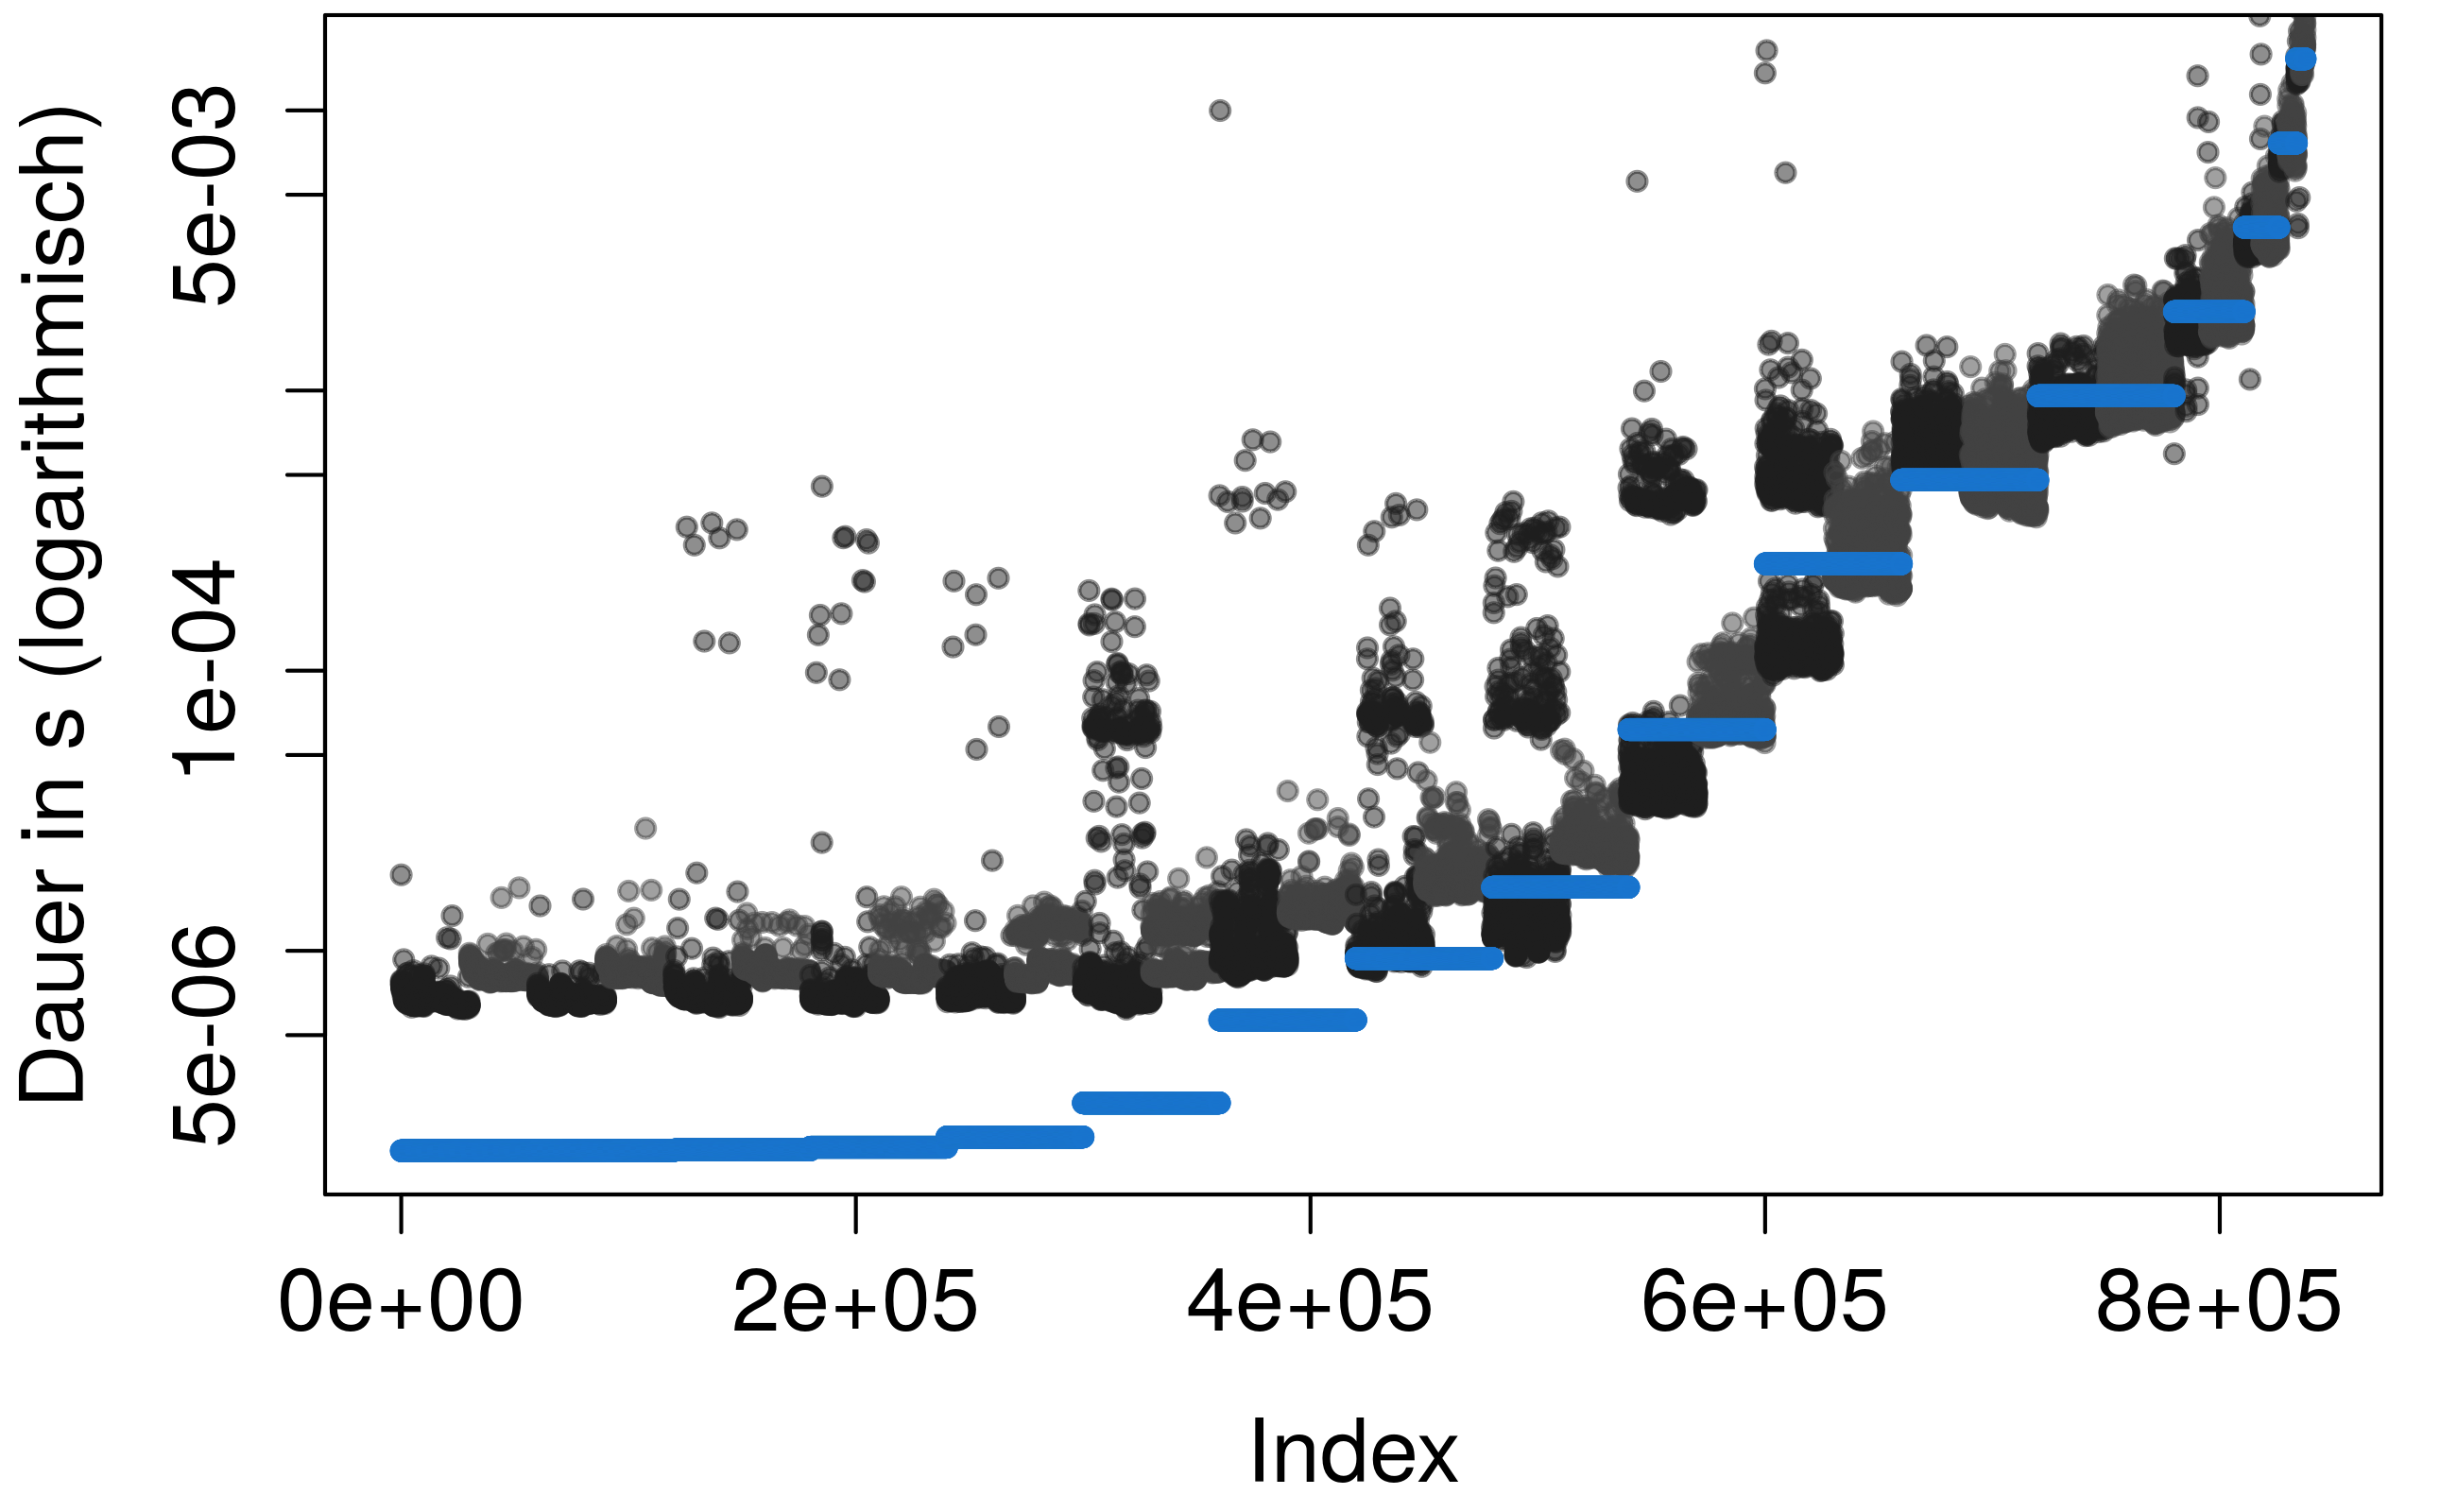
\includegraphics[width=1\linewidth]{Bilder/plot_seq_linreg_Size.png}\\
			\vspace*{-0.45cm}
			\caption{LinReg G}
			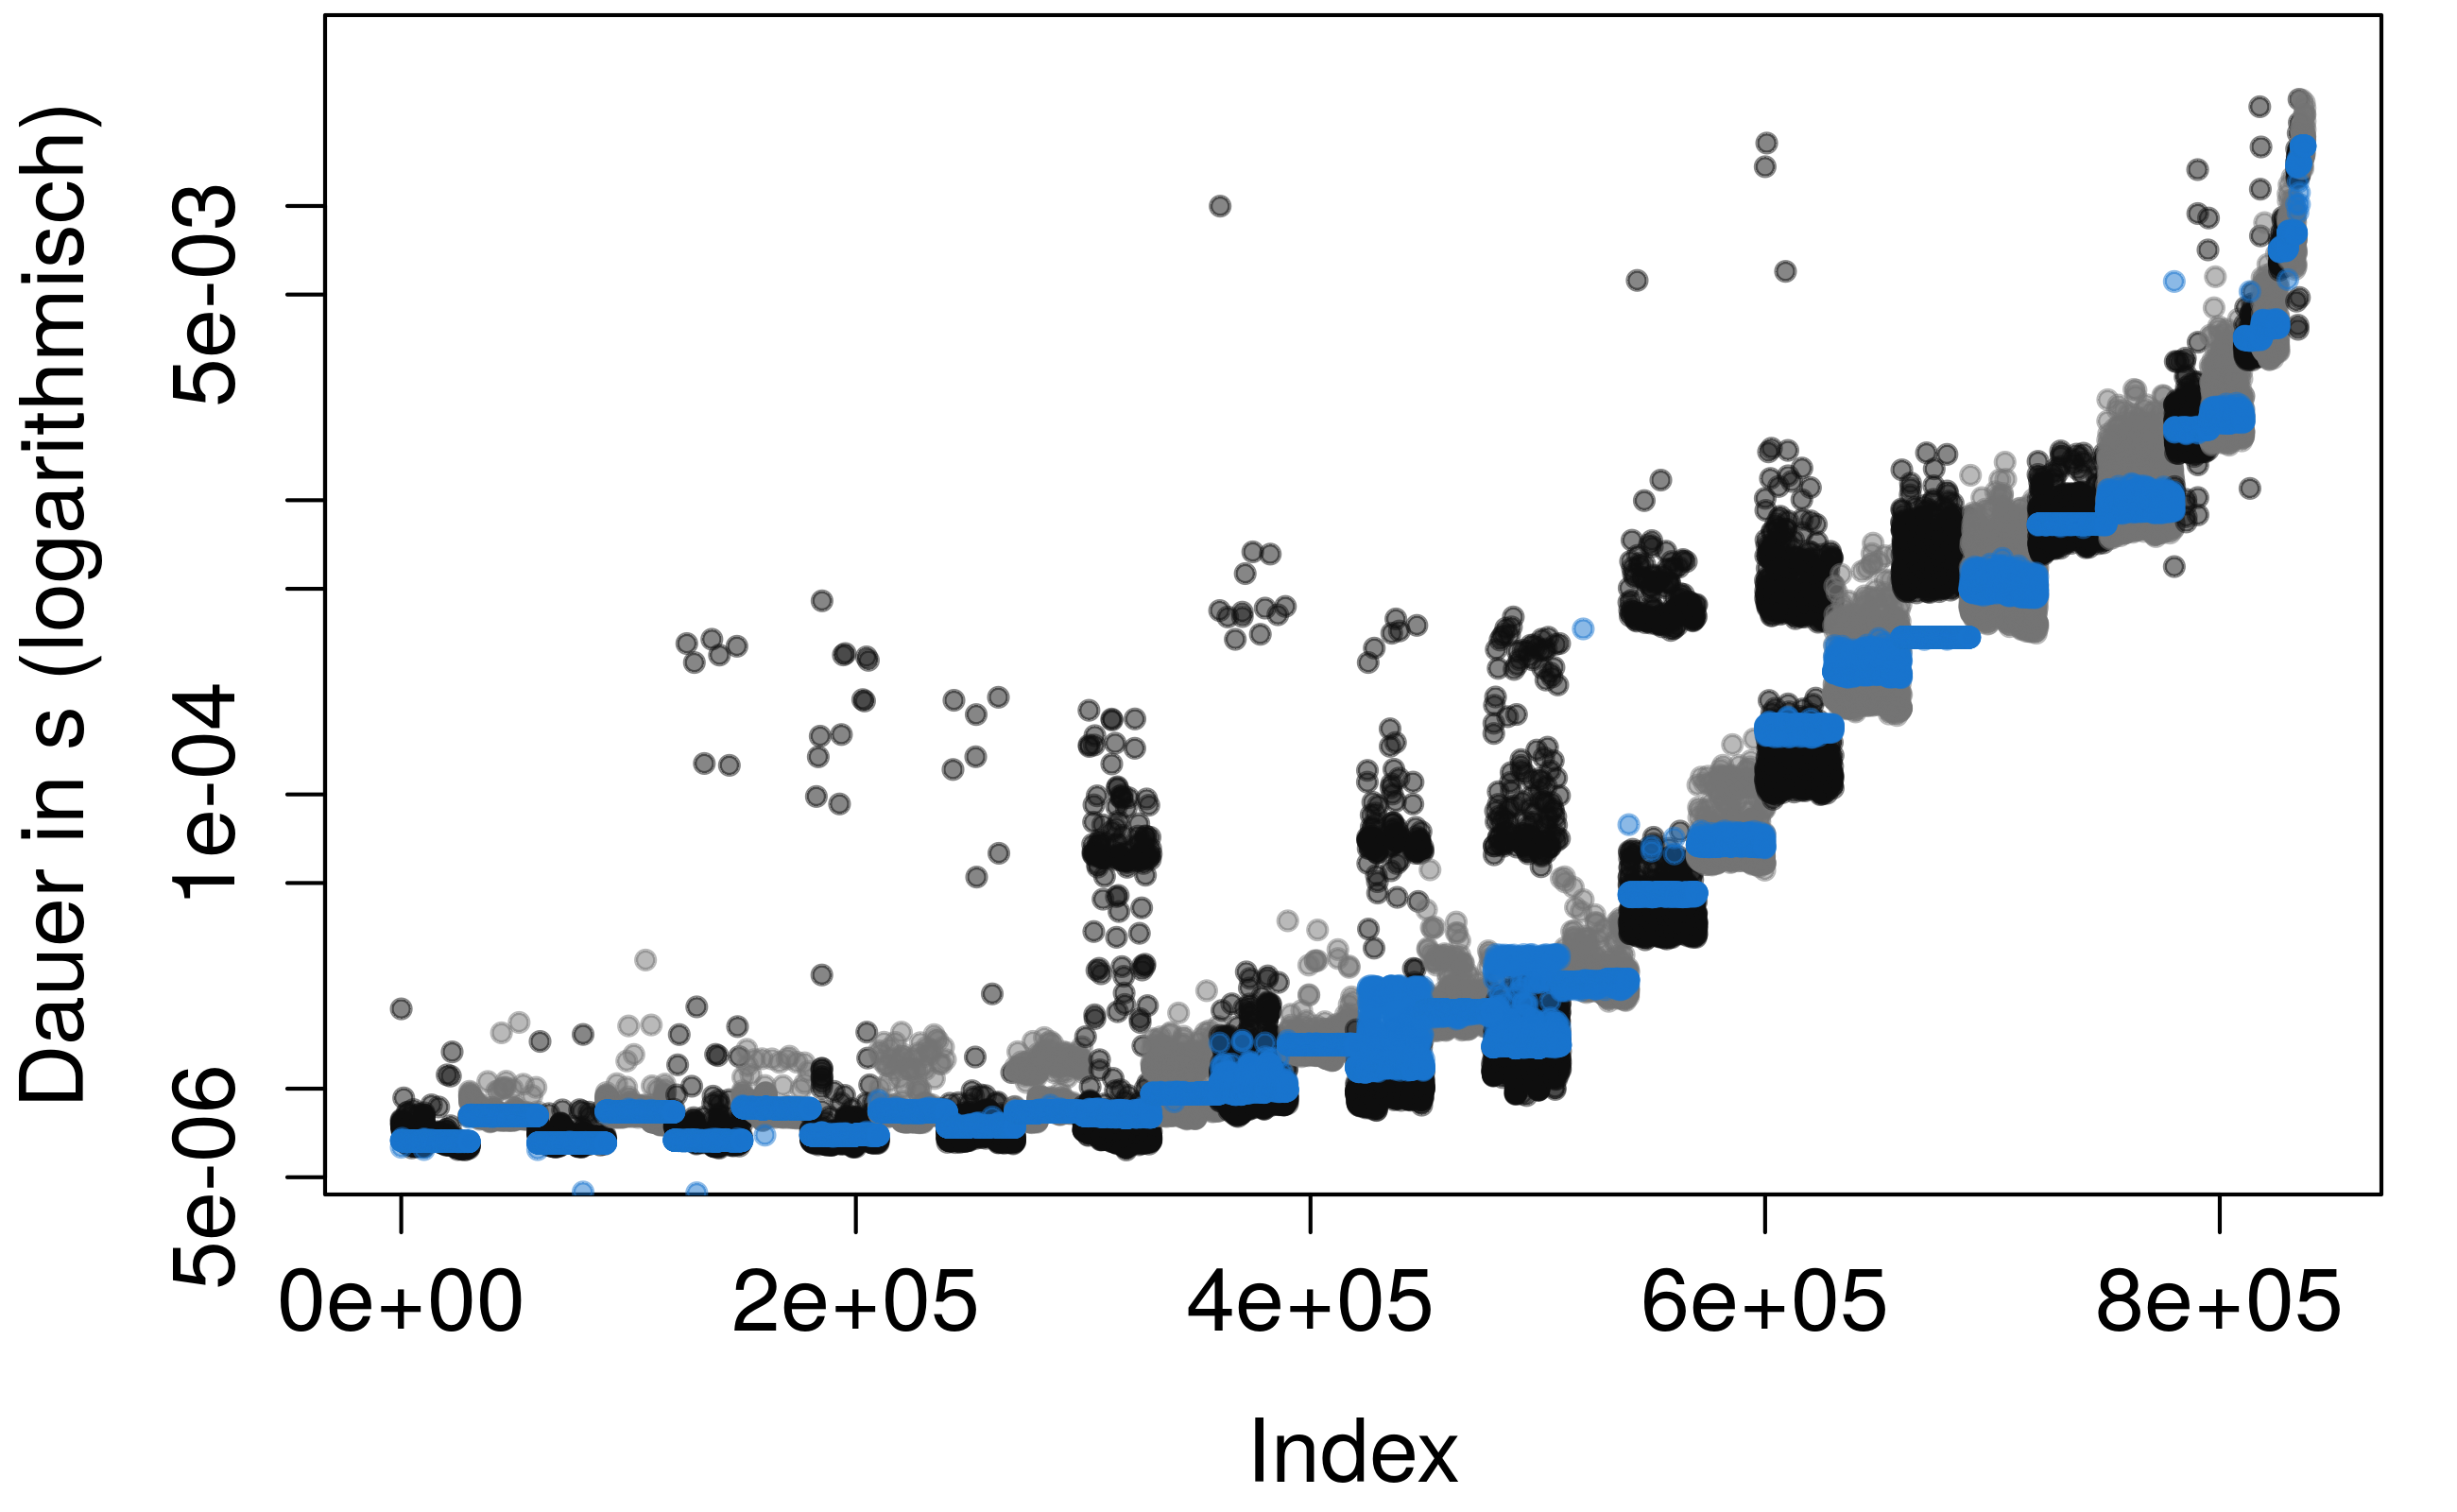
\includegraphics[width=1\linewidth]{Bilder/plot_onlyPred_throughput_ema_Duration_seq.png}
			\vspace*{-0.45cm}
			\caption{NN-EMA}
		\end{figure}
	\end{columns}
\end{frame}

\begin{frame}
\frametitle{Modelle angewendet auf SEQ}
\begin{table}
	\resizebox{\textwidth}{!}{
		\begin{tabular}{|p{2cm}|r|r|r|r|}\hline%
				Modell & MAE\,(s) &  MAPE\,(\%) & MSPE\,(\%) & RMax\,(\%) \\\hline\hline
				\csvreader[late after line=\\\hline]%
				{CSV/latex_seq_results.csv}{Modell=\Model,MAF=\MAF,RMAF=\RMAF, RMQA = \RMQA, Q3 = \Q3, Max = \Max,RMAFTraining = \RMAFTraining, Bereich = \Bereich, RMAFavg = \RMAFavg}%
				{\Model & \MAF & \RMAF & \RMQA & \Max}%
		\end{tabular}
	}
\end{table}
\begin{itemize}
\item MAE: \textit{mean absolute error}
\item MAPE: \textit{mean absolute percentage error}
\item MSPE: \textit{mean square percentage error}
%\item RQ3: drittes Quartil aller relativen Modellabweichungen
\item RMax: maximale relative Modellabweichung
\end{itemize}
\end{frame}

\begin{frame}
	\frametitle{Modelle angewendet auf RND}
	\begin{columns}
		\column{.45\textwidth}
		\begin{figure}
			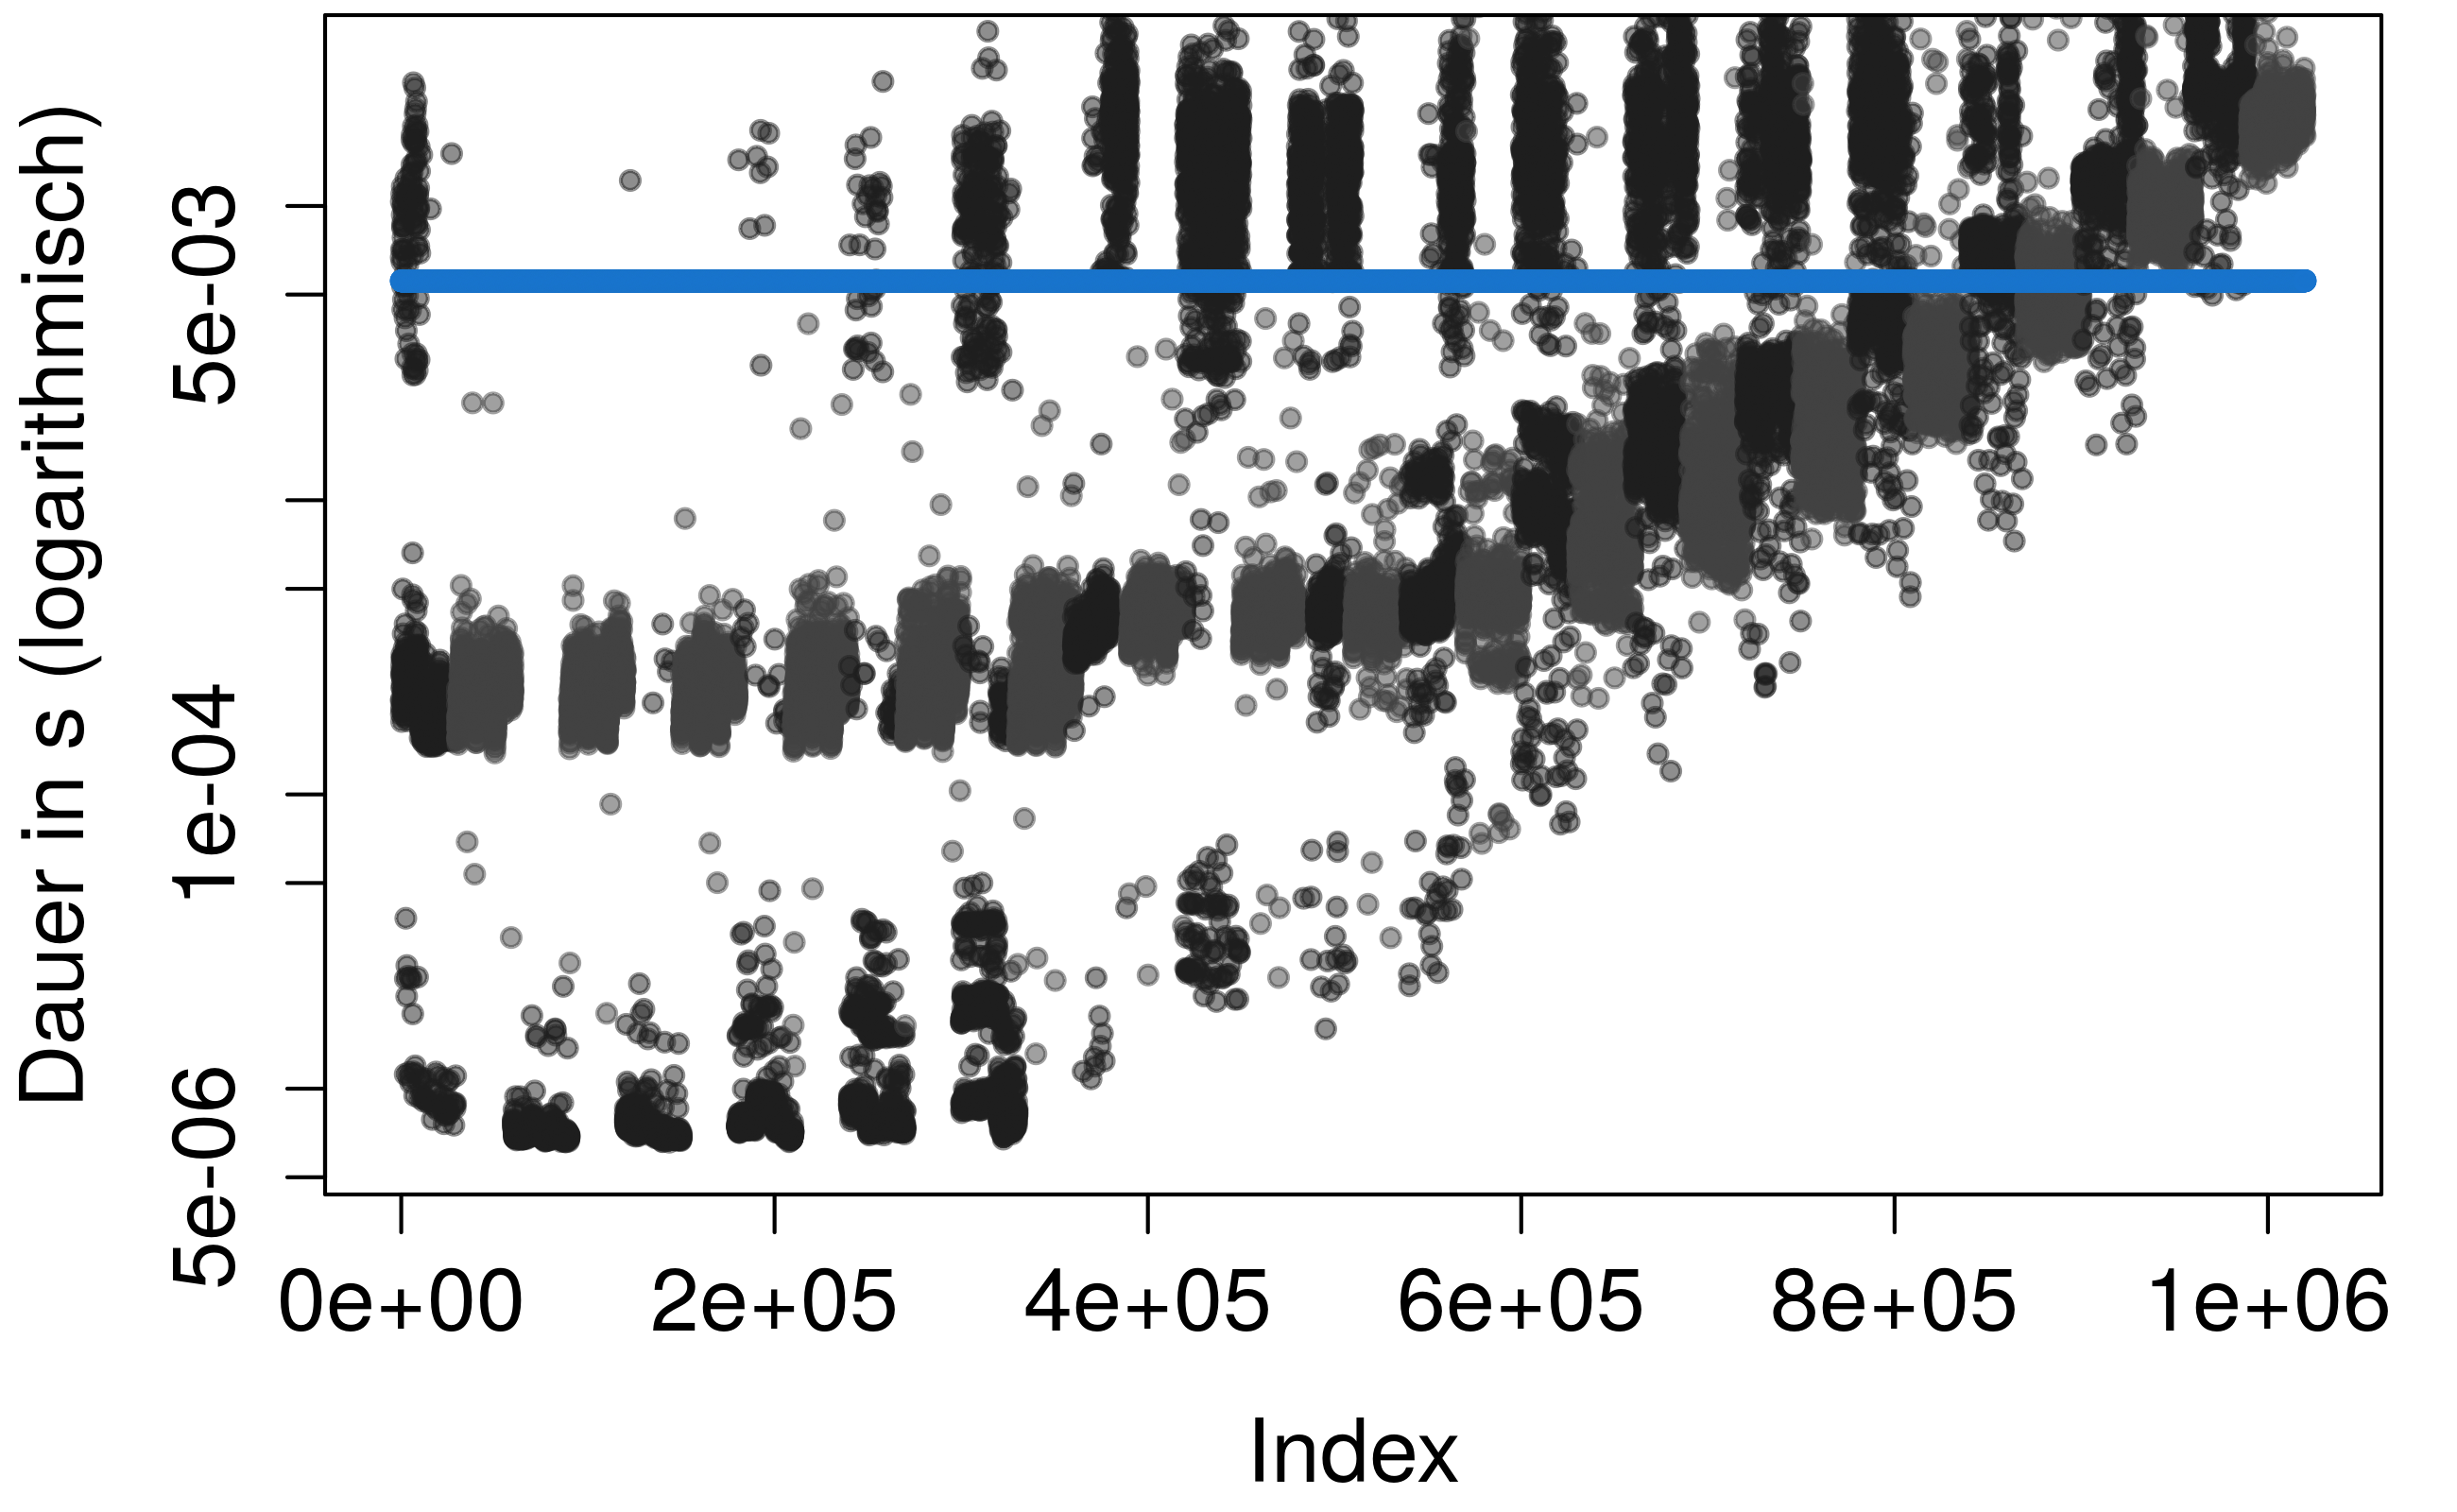
\includegraphics[width=1\linewidth]{Bilder/plot_rnd_mean_performance.png}\\
			\vspace*{-0.45cm}
			\caption{Durchschnitt}
			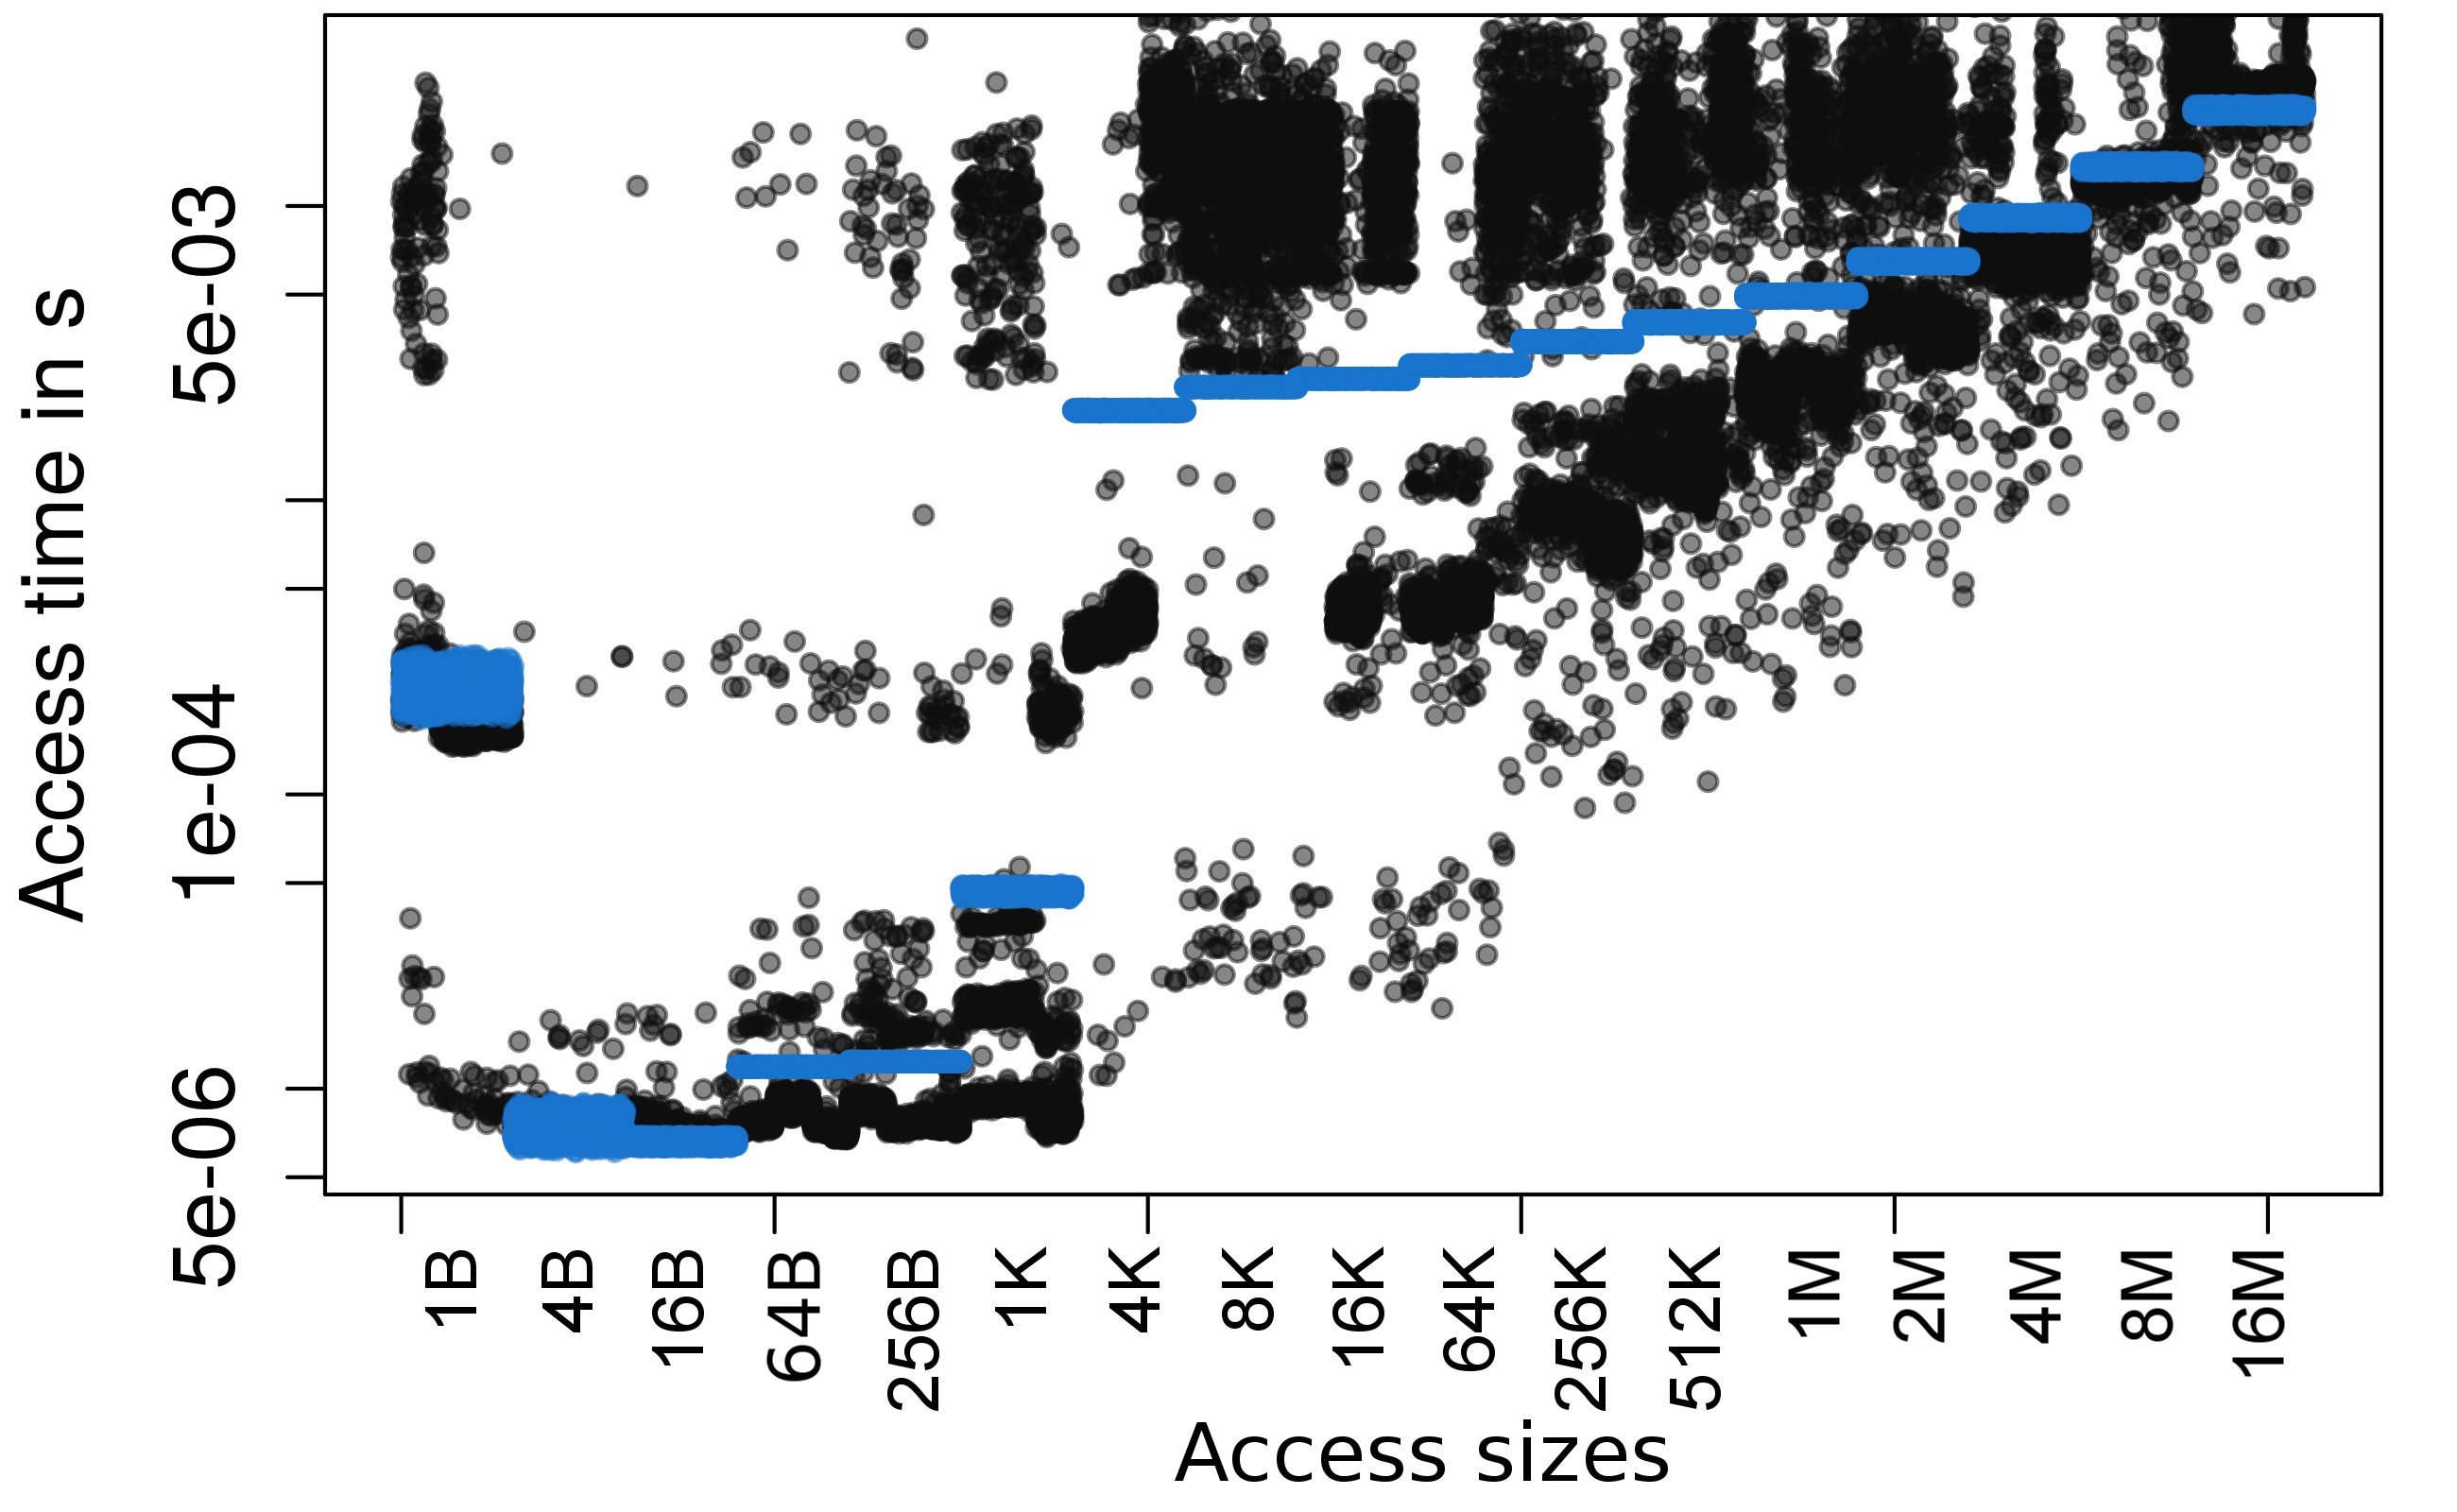
\includegraphics[width=1\linewidth]{Bilder/plot_onlyPred_tuple1_Duration_rnd.png}
			\vspace*{-0.45cm}
			\caption{NN-Tupel1}
		\end{figure}
		\column{.45\textwidth}
		\begin{figure}
			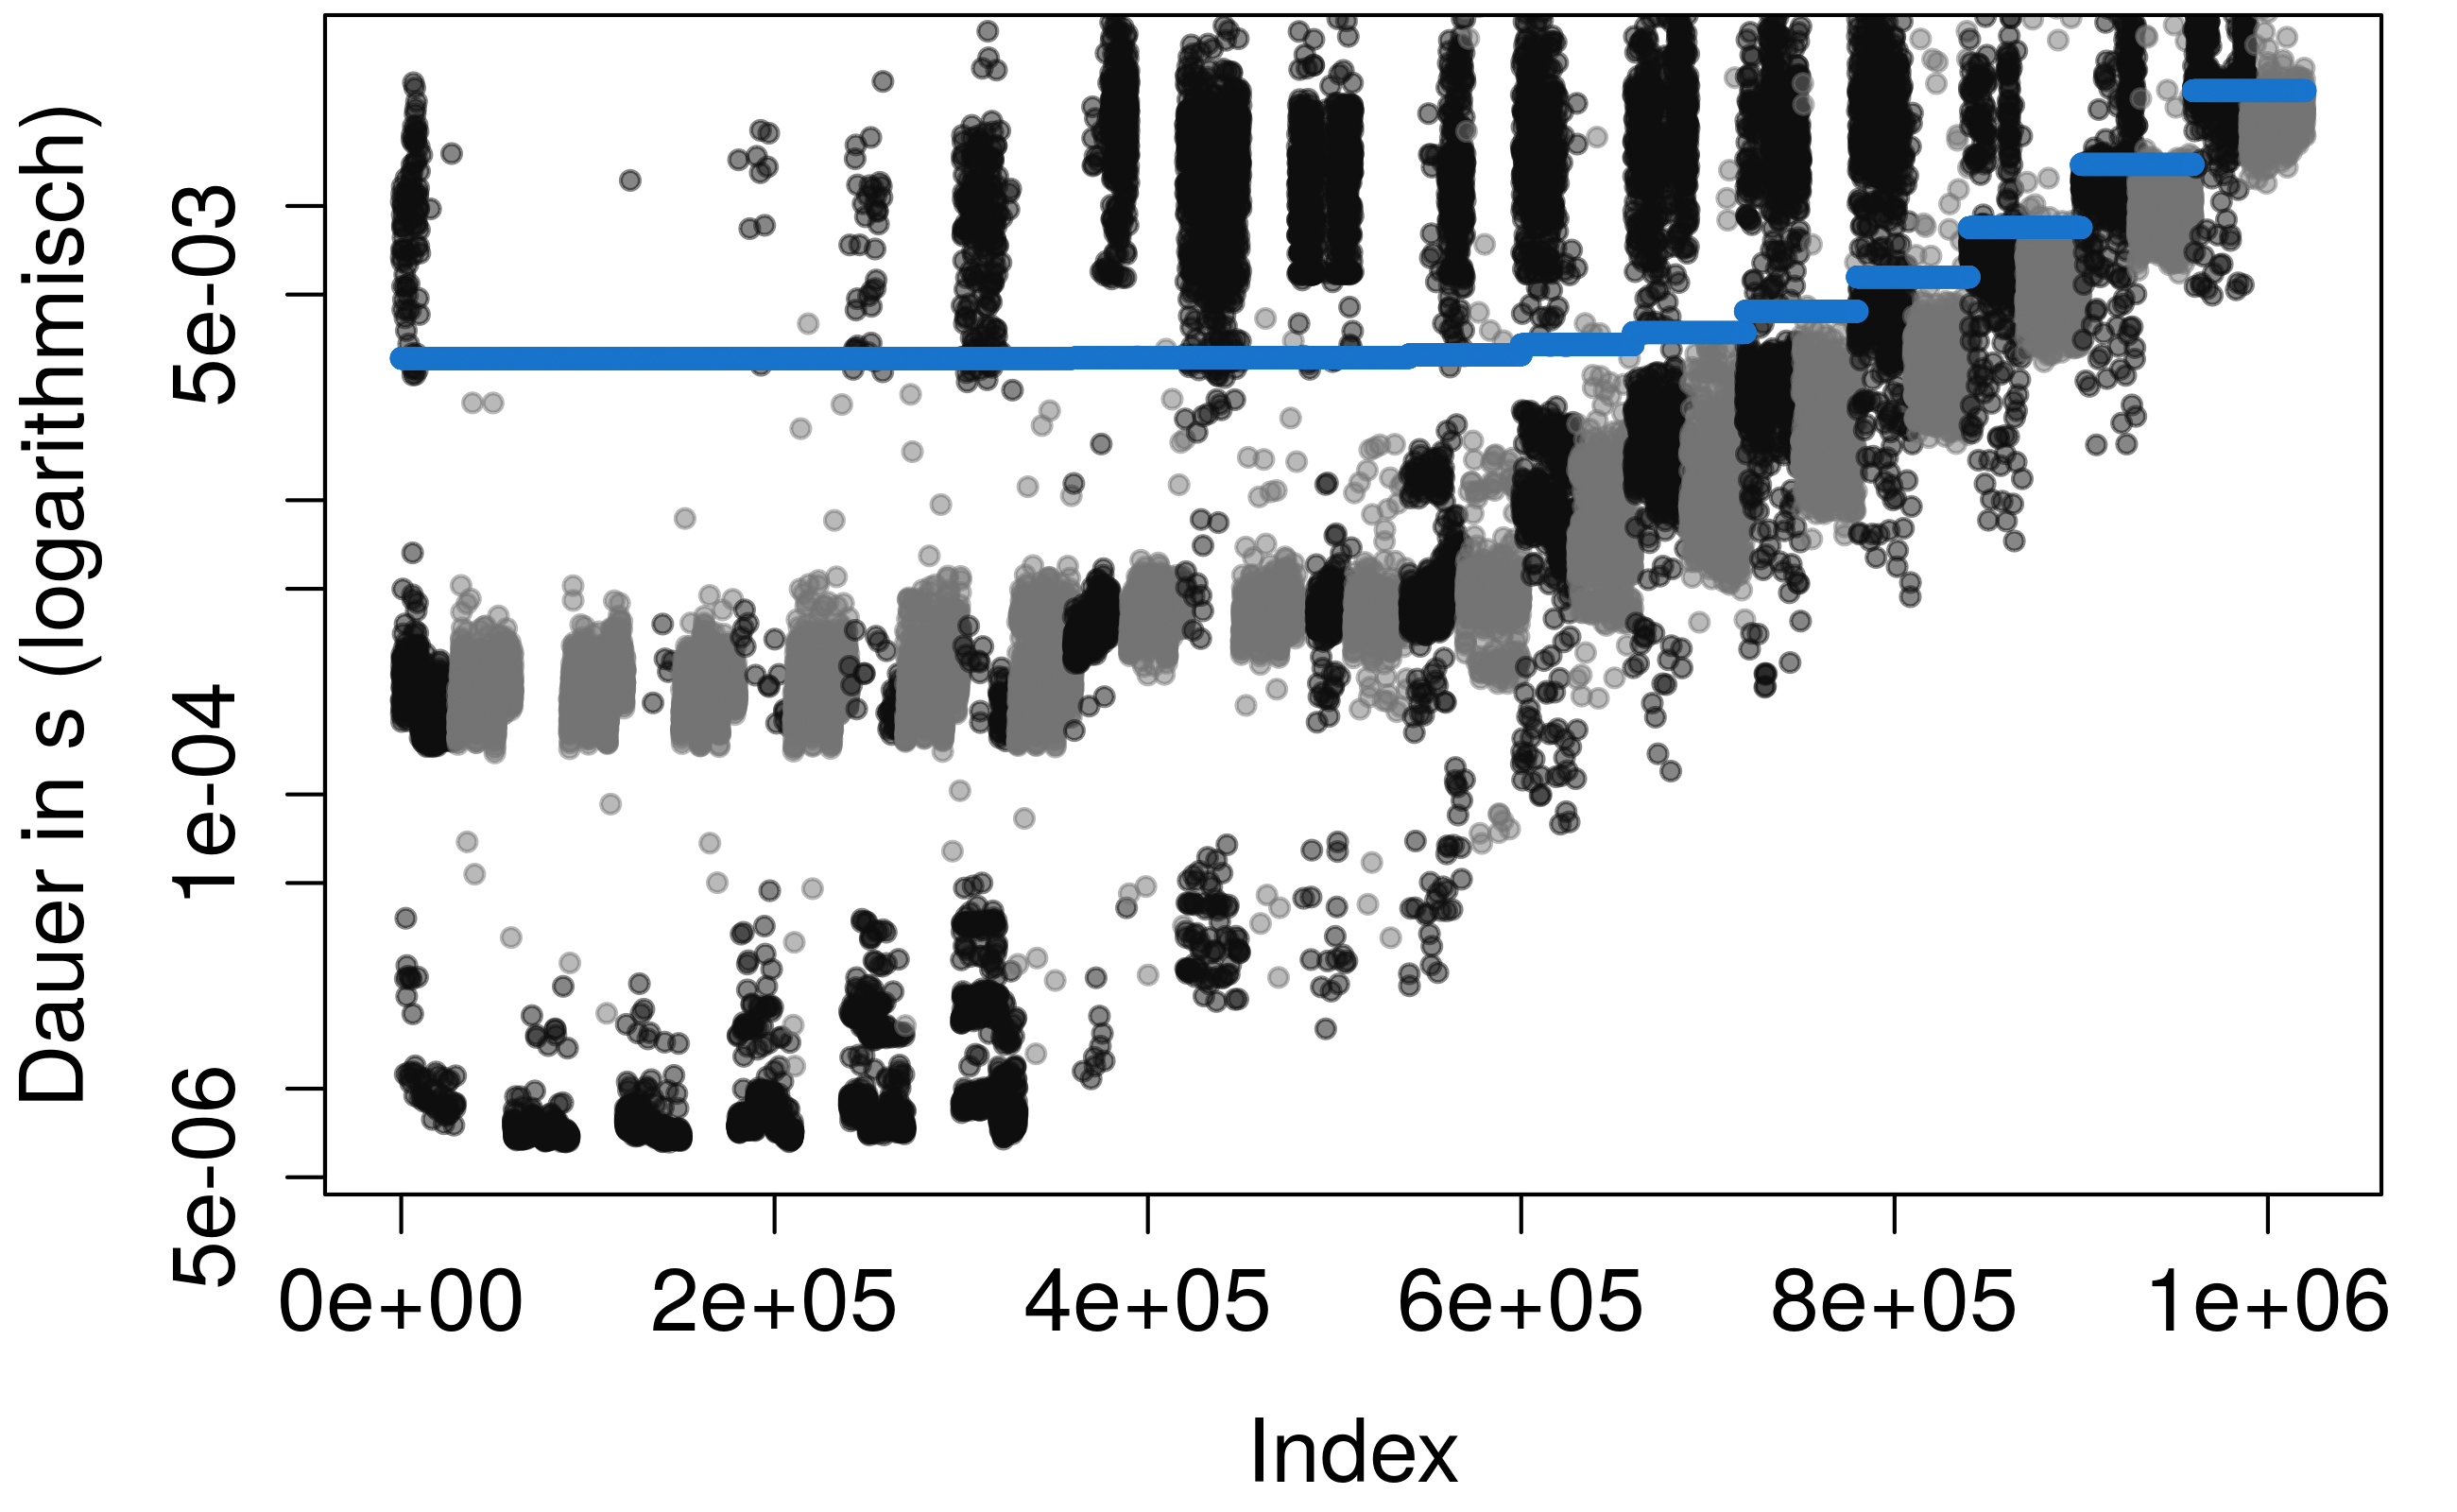
\includegraphics[width=1\linewidth]{Bilder/plot_rnd_linreg_Size.png}\\
			\vspace*{-0.45cm}
			\caption{LinReg G}
			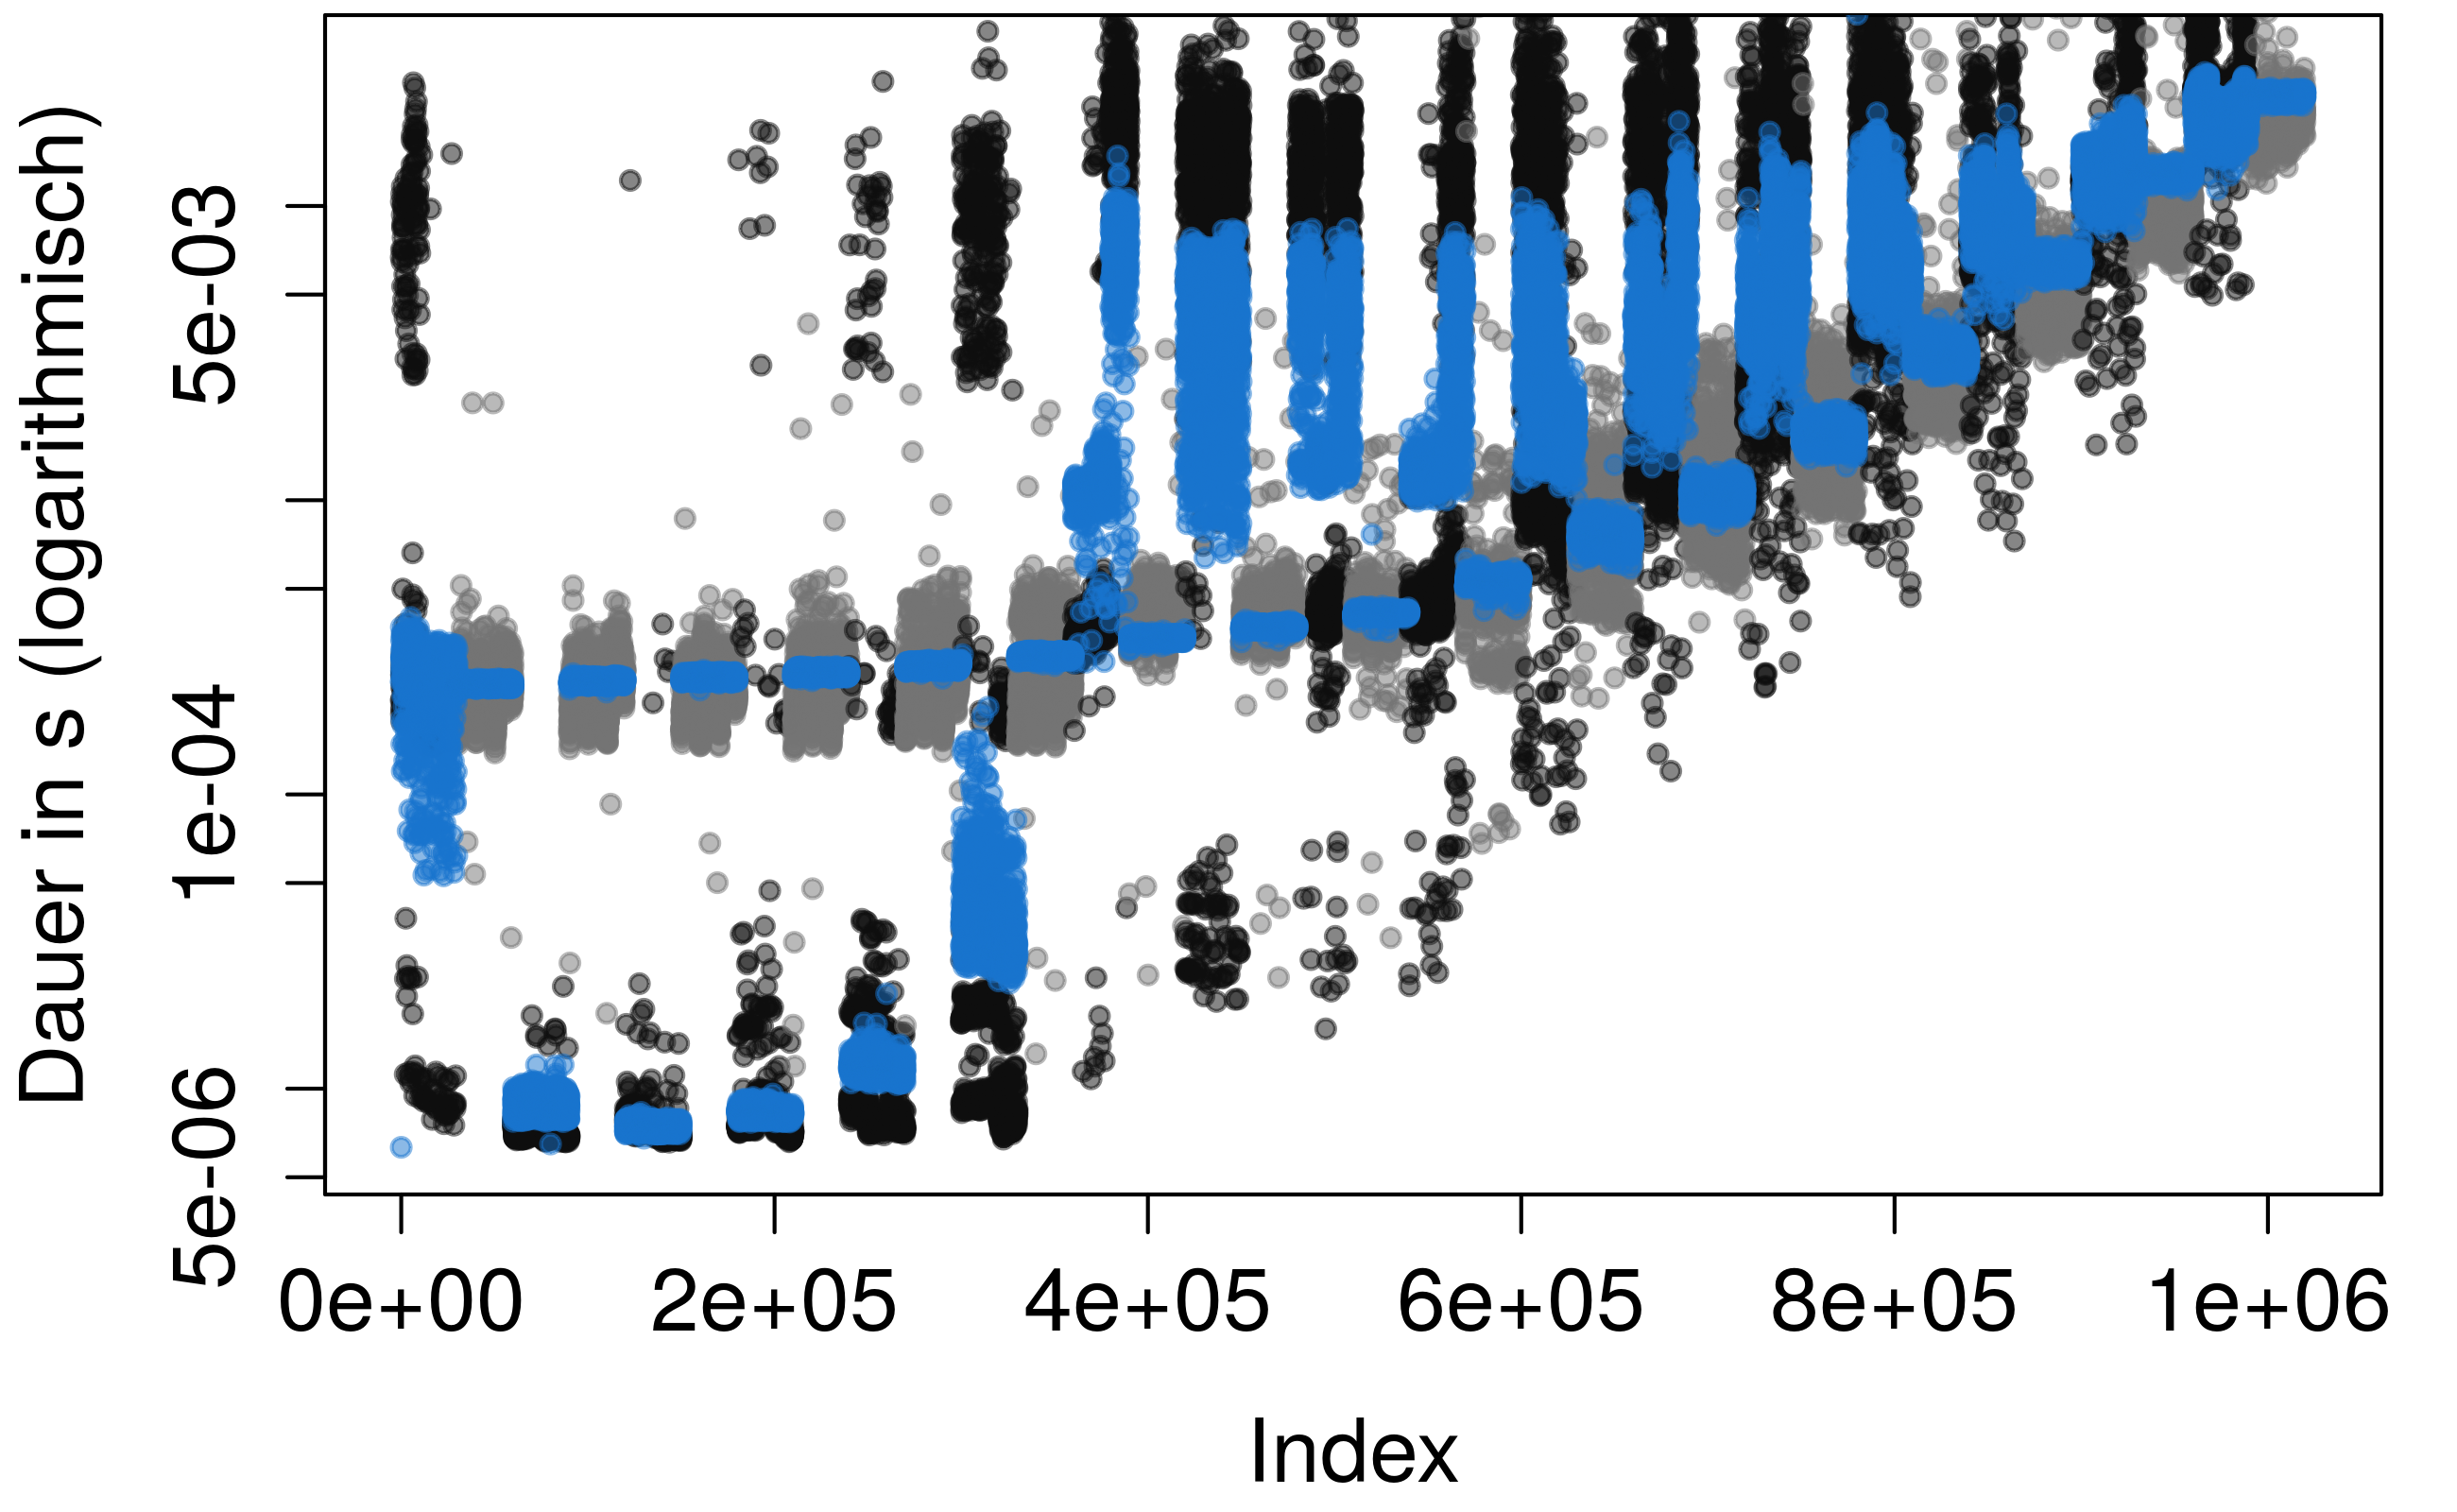
\includegraphics[width=1\linewidth]{Bilder/plot_onlyPred_throughput_ema_Duration_rnd.png}
			\vspace*{-0.45cm}
			\caption{NN-EMA}
		\end{figure}
	\end{columns}
\end{frame}

\begin{frame}
\frametitle{Modelle angewendet auf RND}
\begin{table}
	\resizebox{\textwidth}{!}{
		\begin{tabular}{|p{2cm}|r|r|r|r|}\hline%
				Modell & MAE\,(s) & MAPE\,(\%) & MSPE\,(\%) & RMax\,(\%) \\\hline\hline
			\csvreader[late after line=\\\hline]%
				{CSV/latex_rnd_results.csv}{Modell=\Model,MAF=\MAF,RMAF=\RMAF, RMQA = \RMQA, Q3 = \Q3, Max = \Max,RMAFTraining = \RMAFTraining, Bereich = \Bereich, RMAFavg = \RMAFavg}%
				{\Model & \MAF & \RMAF & \RMQA & \Max}%
		\end{tabular}
	}
\end{table}
\begin{itemize}
\item MAE: \textit{mean absolute error}
\item MAPE: \textit{mean absolute percentage error}
\item MSPE: \textit{mean square percentage error}
%\item RQ3: drittes Quartil aller relativen Modellabweichungen
\item RMax: maximale relative Modellabweichung
\end{itemize}
\end{frame}

\section{Näherung des E/A-Pfads bestimmen}
\begin{frame}
\frametitle{Näherung des E/A-Pfads bestimmen}
%Entdeckt, dass E/A-Pfad sehr wichtig für korrekte Vorhersage sein sollte
%auch interessant zu wissen
\begin{itemize}
	\item Für ein gutes Modell: Näherung des E/A-Pfads
	\item \textbf{Idee}: Residuen eines einfachen Modells zur Bestimmung einer Näherung des E/A-Pfades eines Dateizugriffs nutzen
	\item Clustering der Residuen zu \textbf{Fehlerklassen} 
	%\item Problem: Höhere Zugriffszeiten führen zu größeren Modellabweichungen
	%bei SEQ deutliches Problem, bei RND nicht mehr so stark
\end{itemize}
\end{frame}
\subsection{Fehlerklassen}
%Nur Betrachtung von LinReg Fehlern!
\begin{frame}
\frametitle{Fehlerklassen auf SEQ}
\begin{columns}
\column{.45\textwidth}
	\begin{figure}
		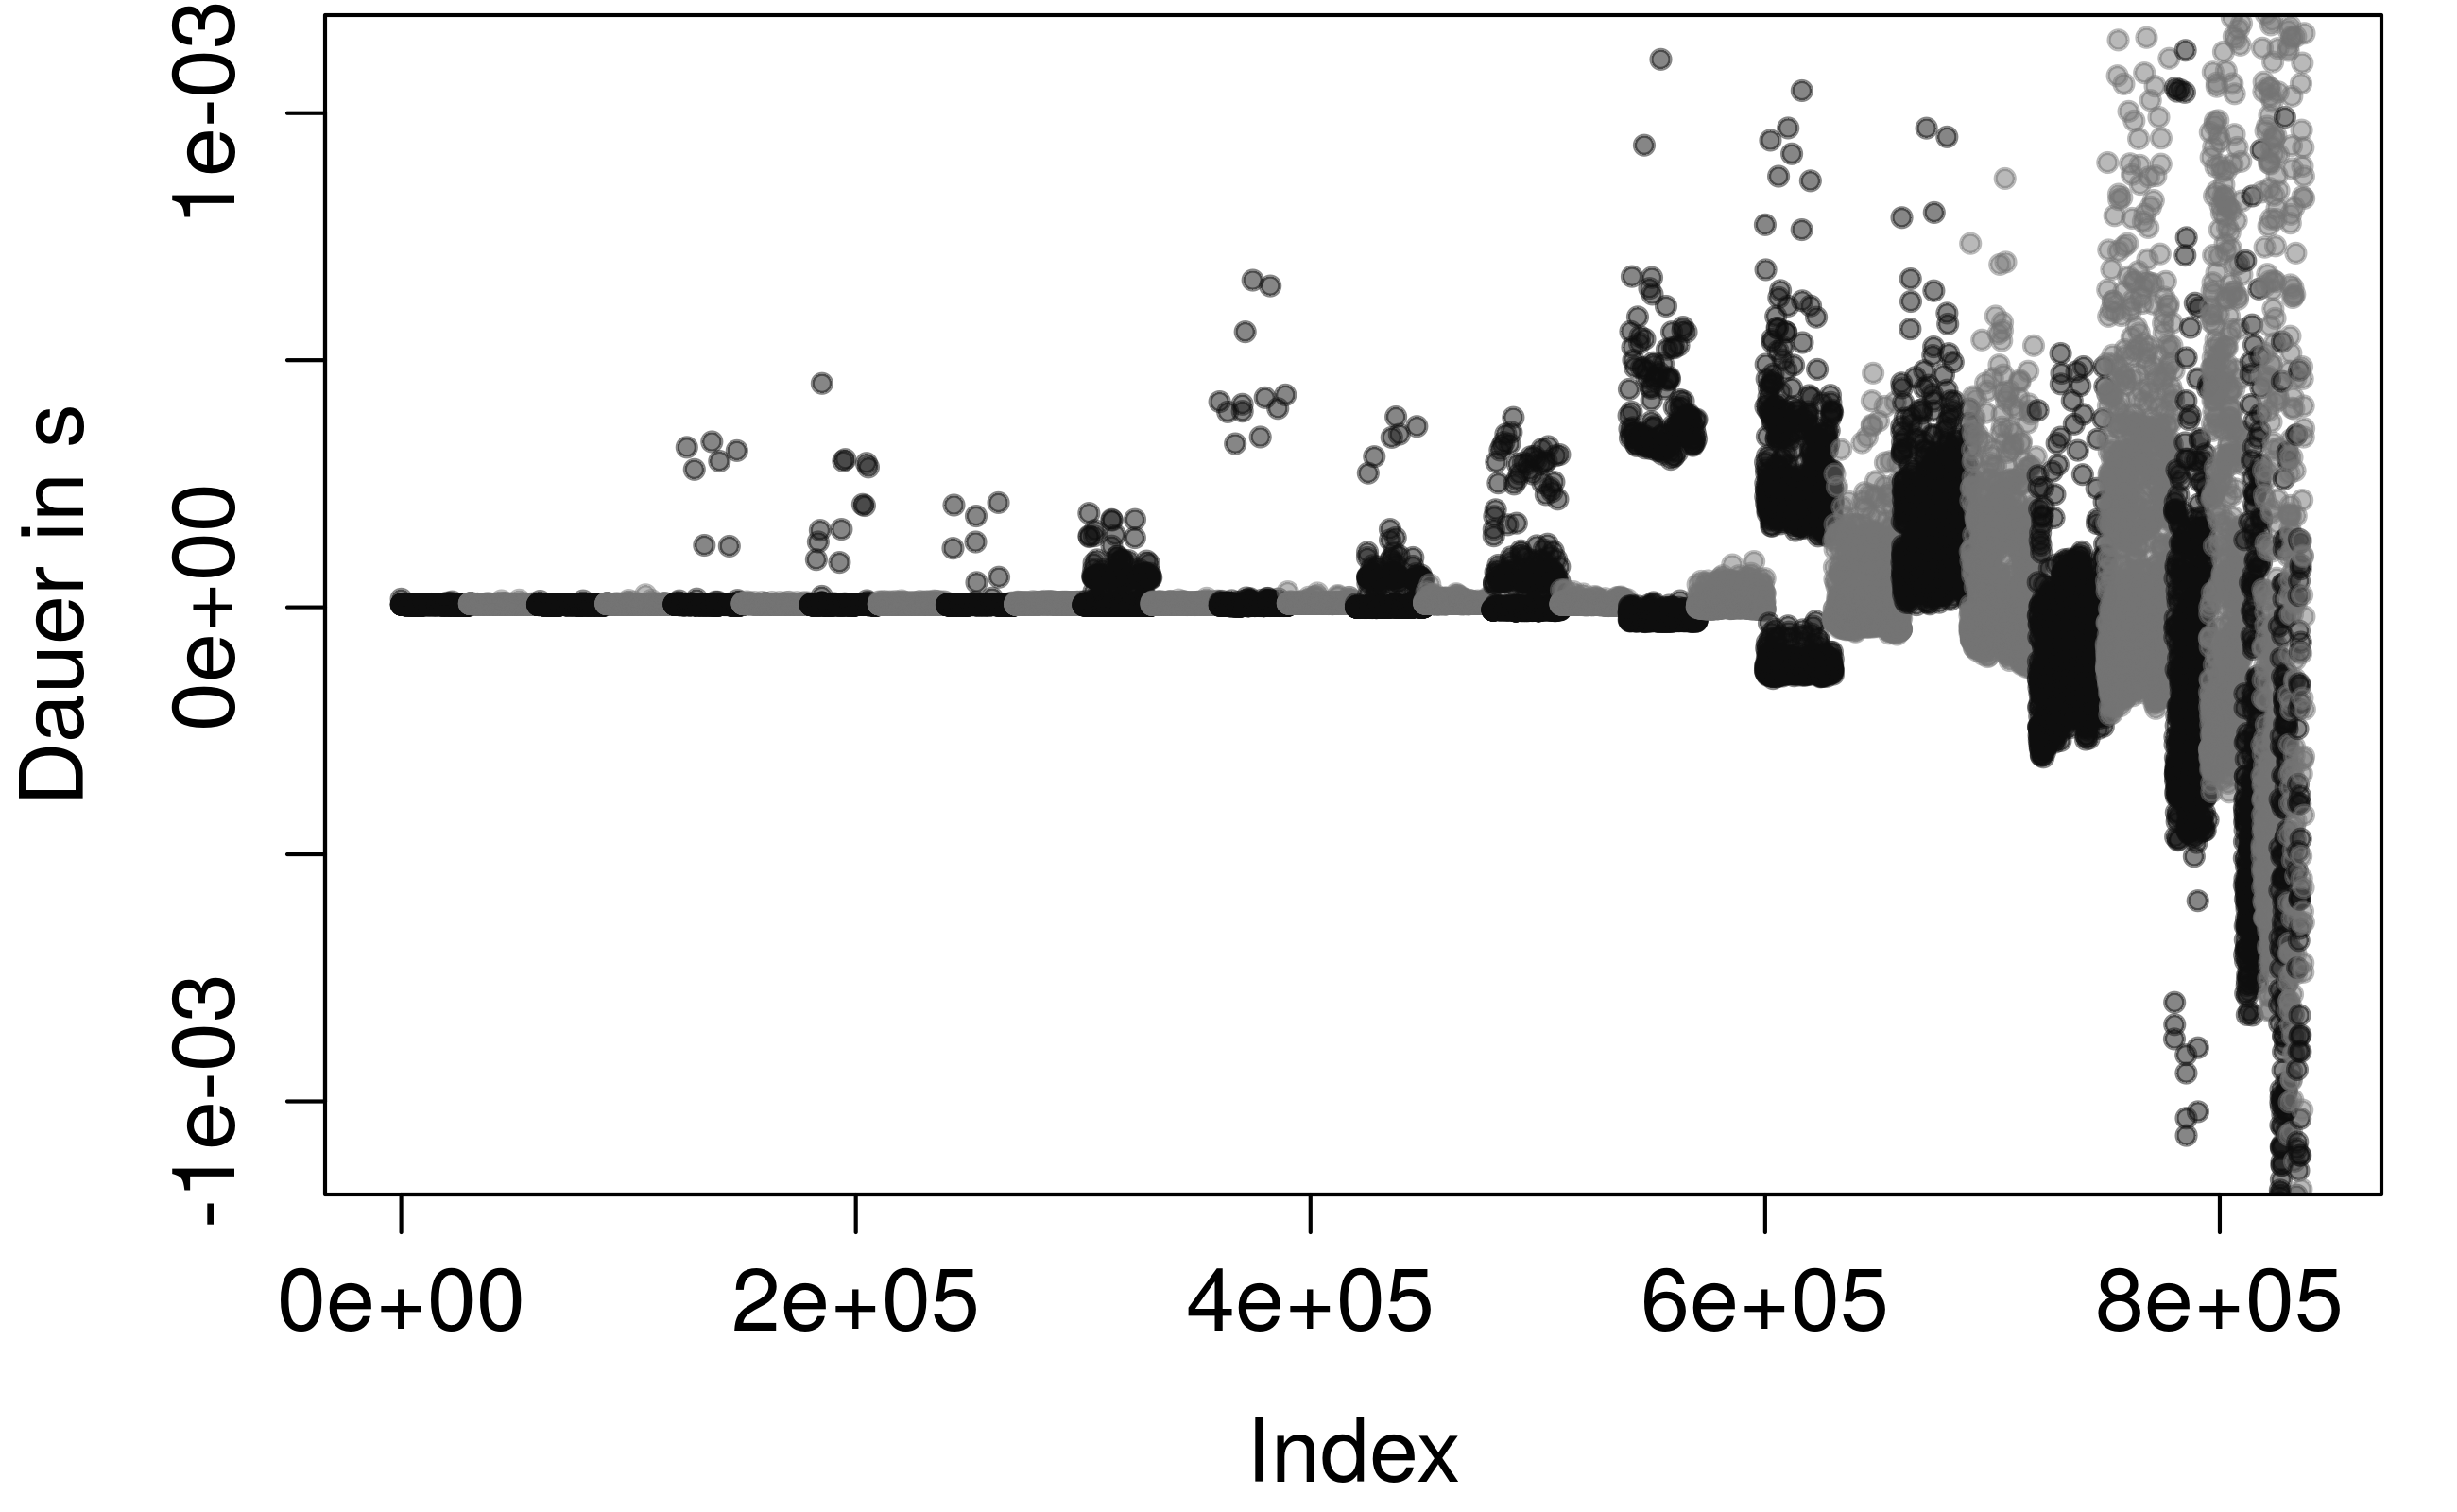
\includegraphics[width=1\linewidth]{Bilder/linreg_error_seq_all.png}\\
		\vspace*{-0.45cm}
		\caption{Residuen von LinReg G auf SEQ}
		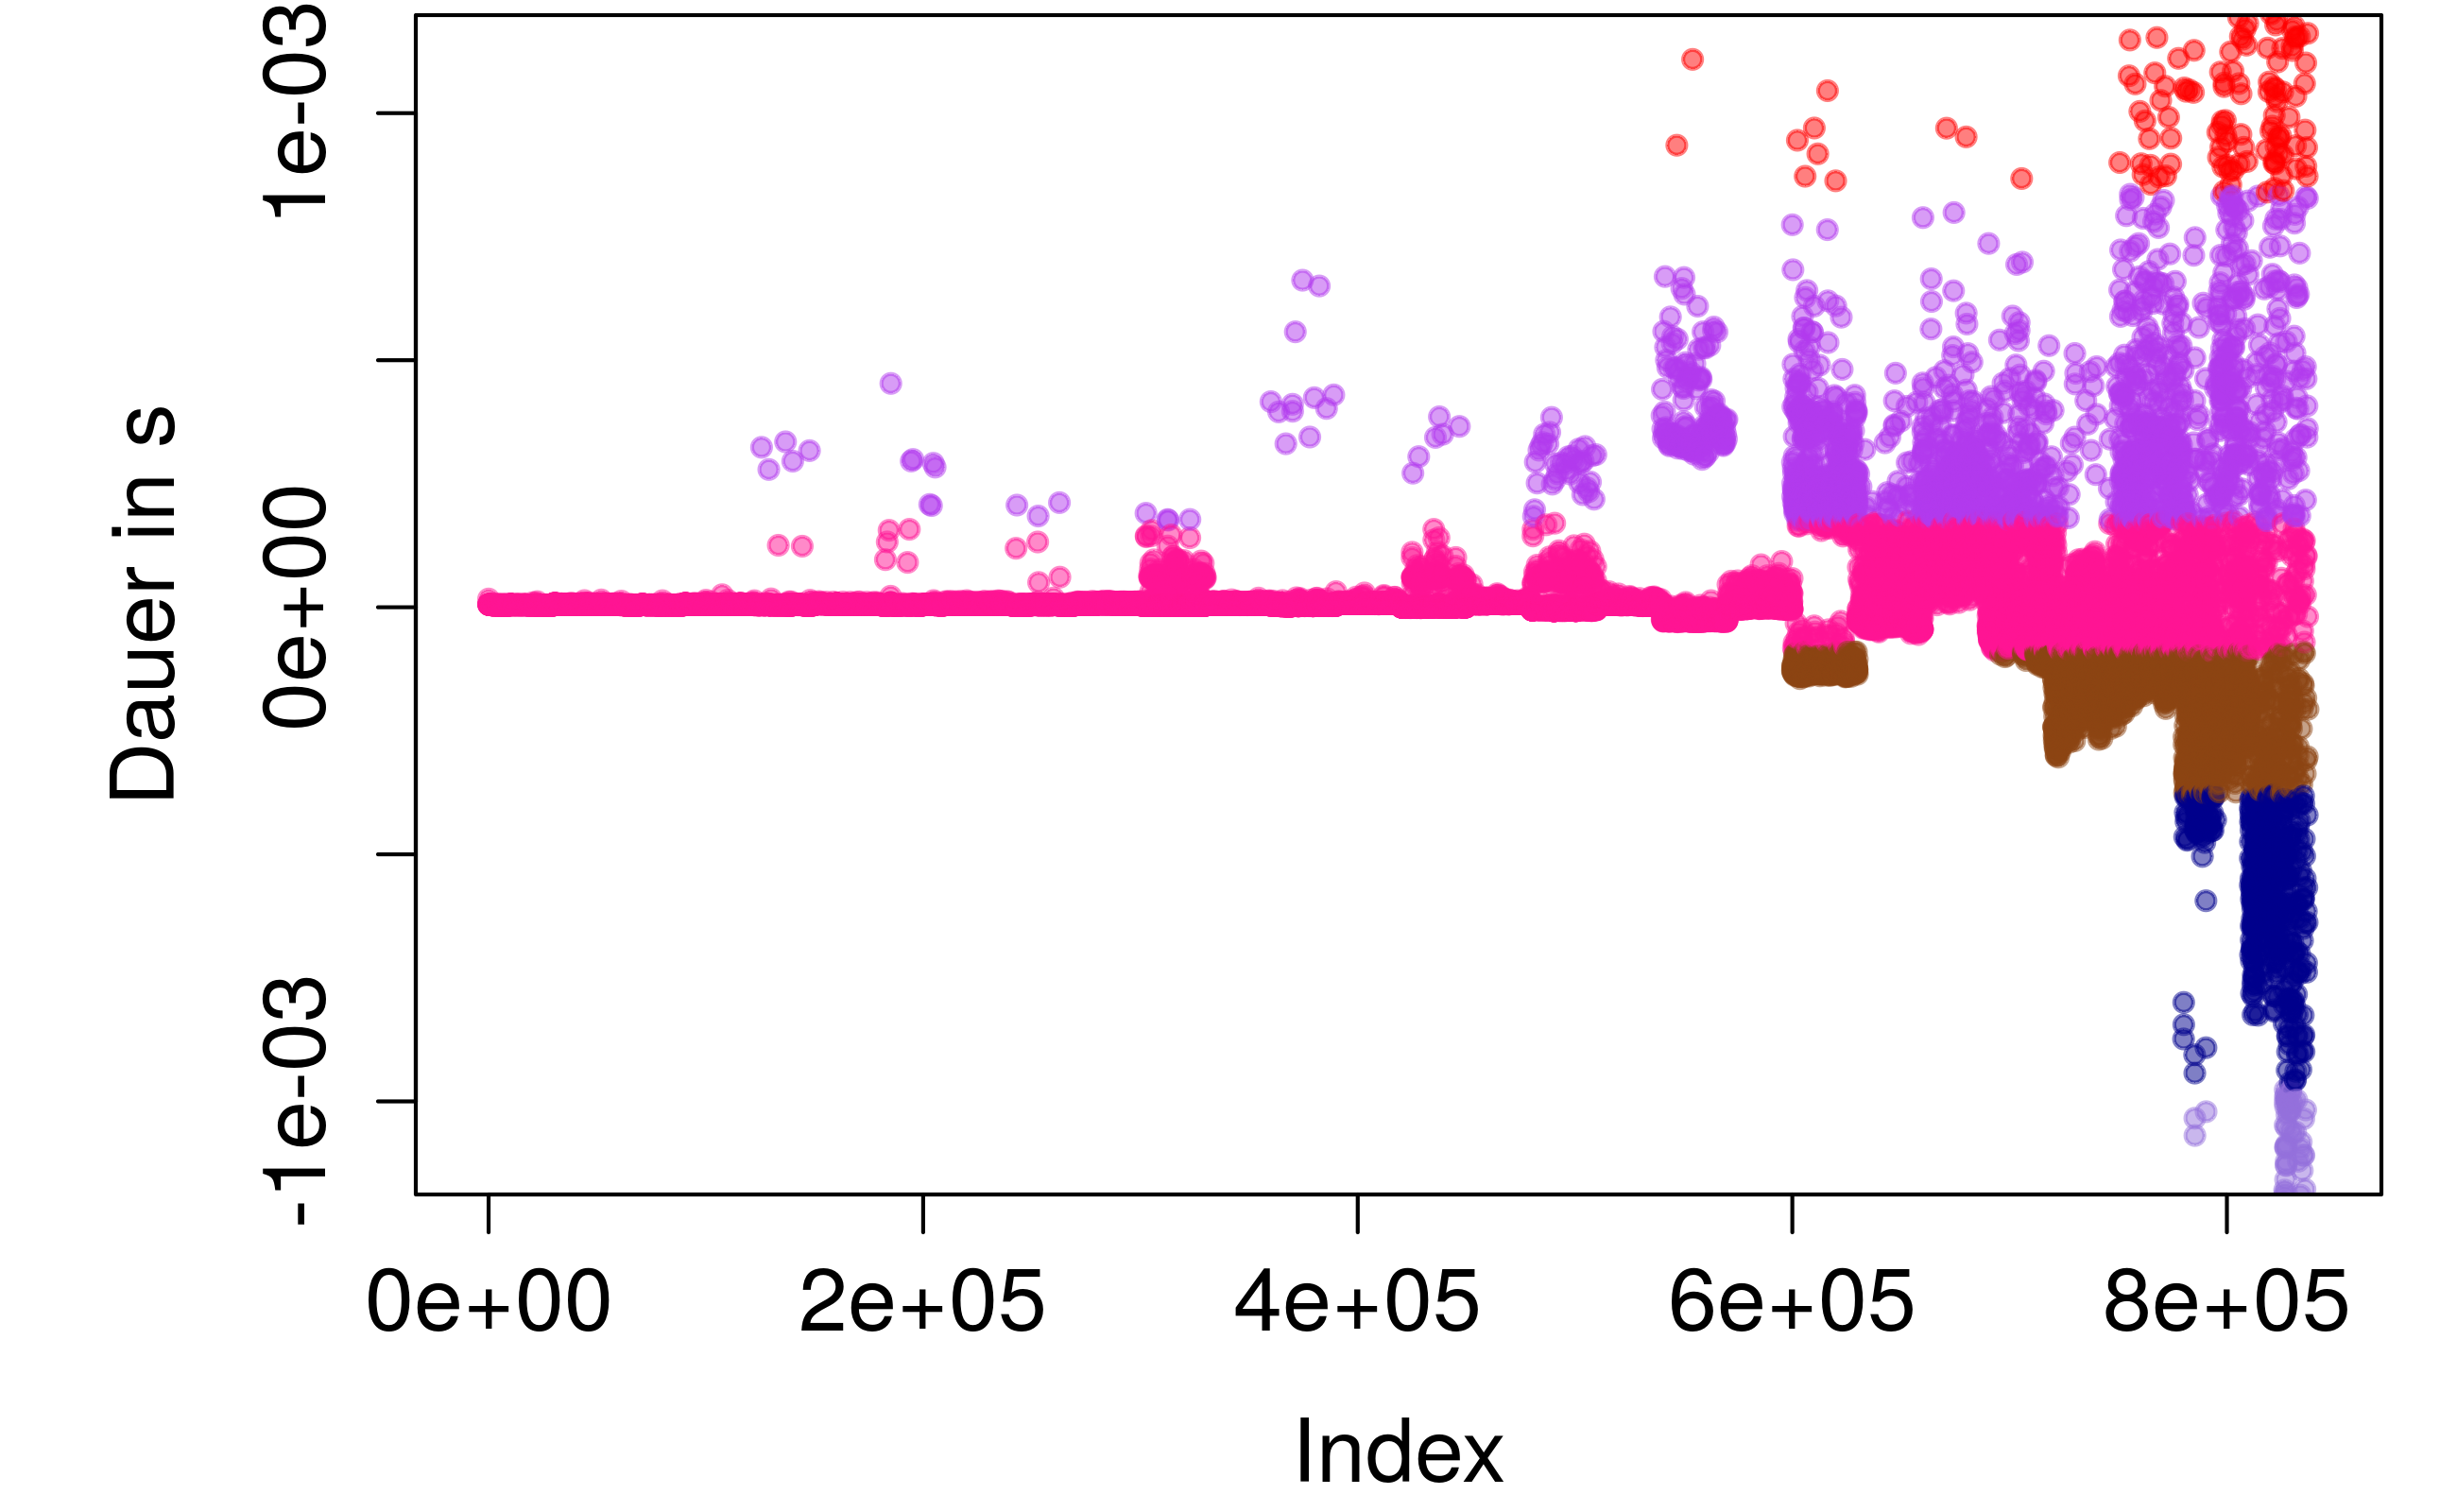
\includegraphics[width=1\linewidth]{Bilder/linreg_error_clustering_seq_all.png}\\
		\vspace*{-0.45cm}
		\caption{Farblich markierte Fehlerklassen}
	\end{figure}
\column{.45\textwidth}
	\begin{figure}		
		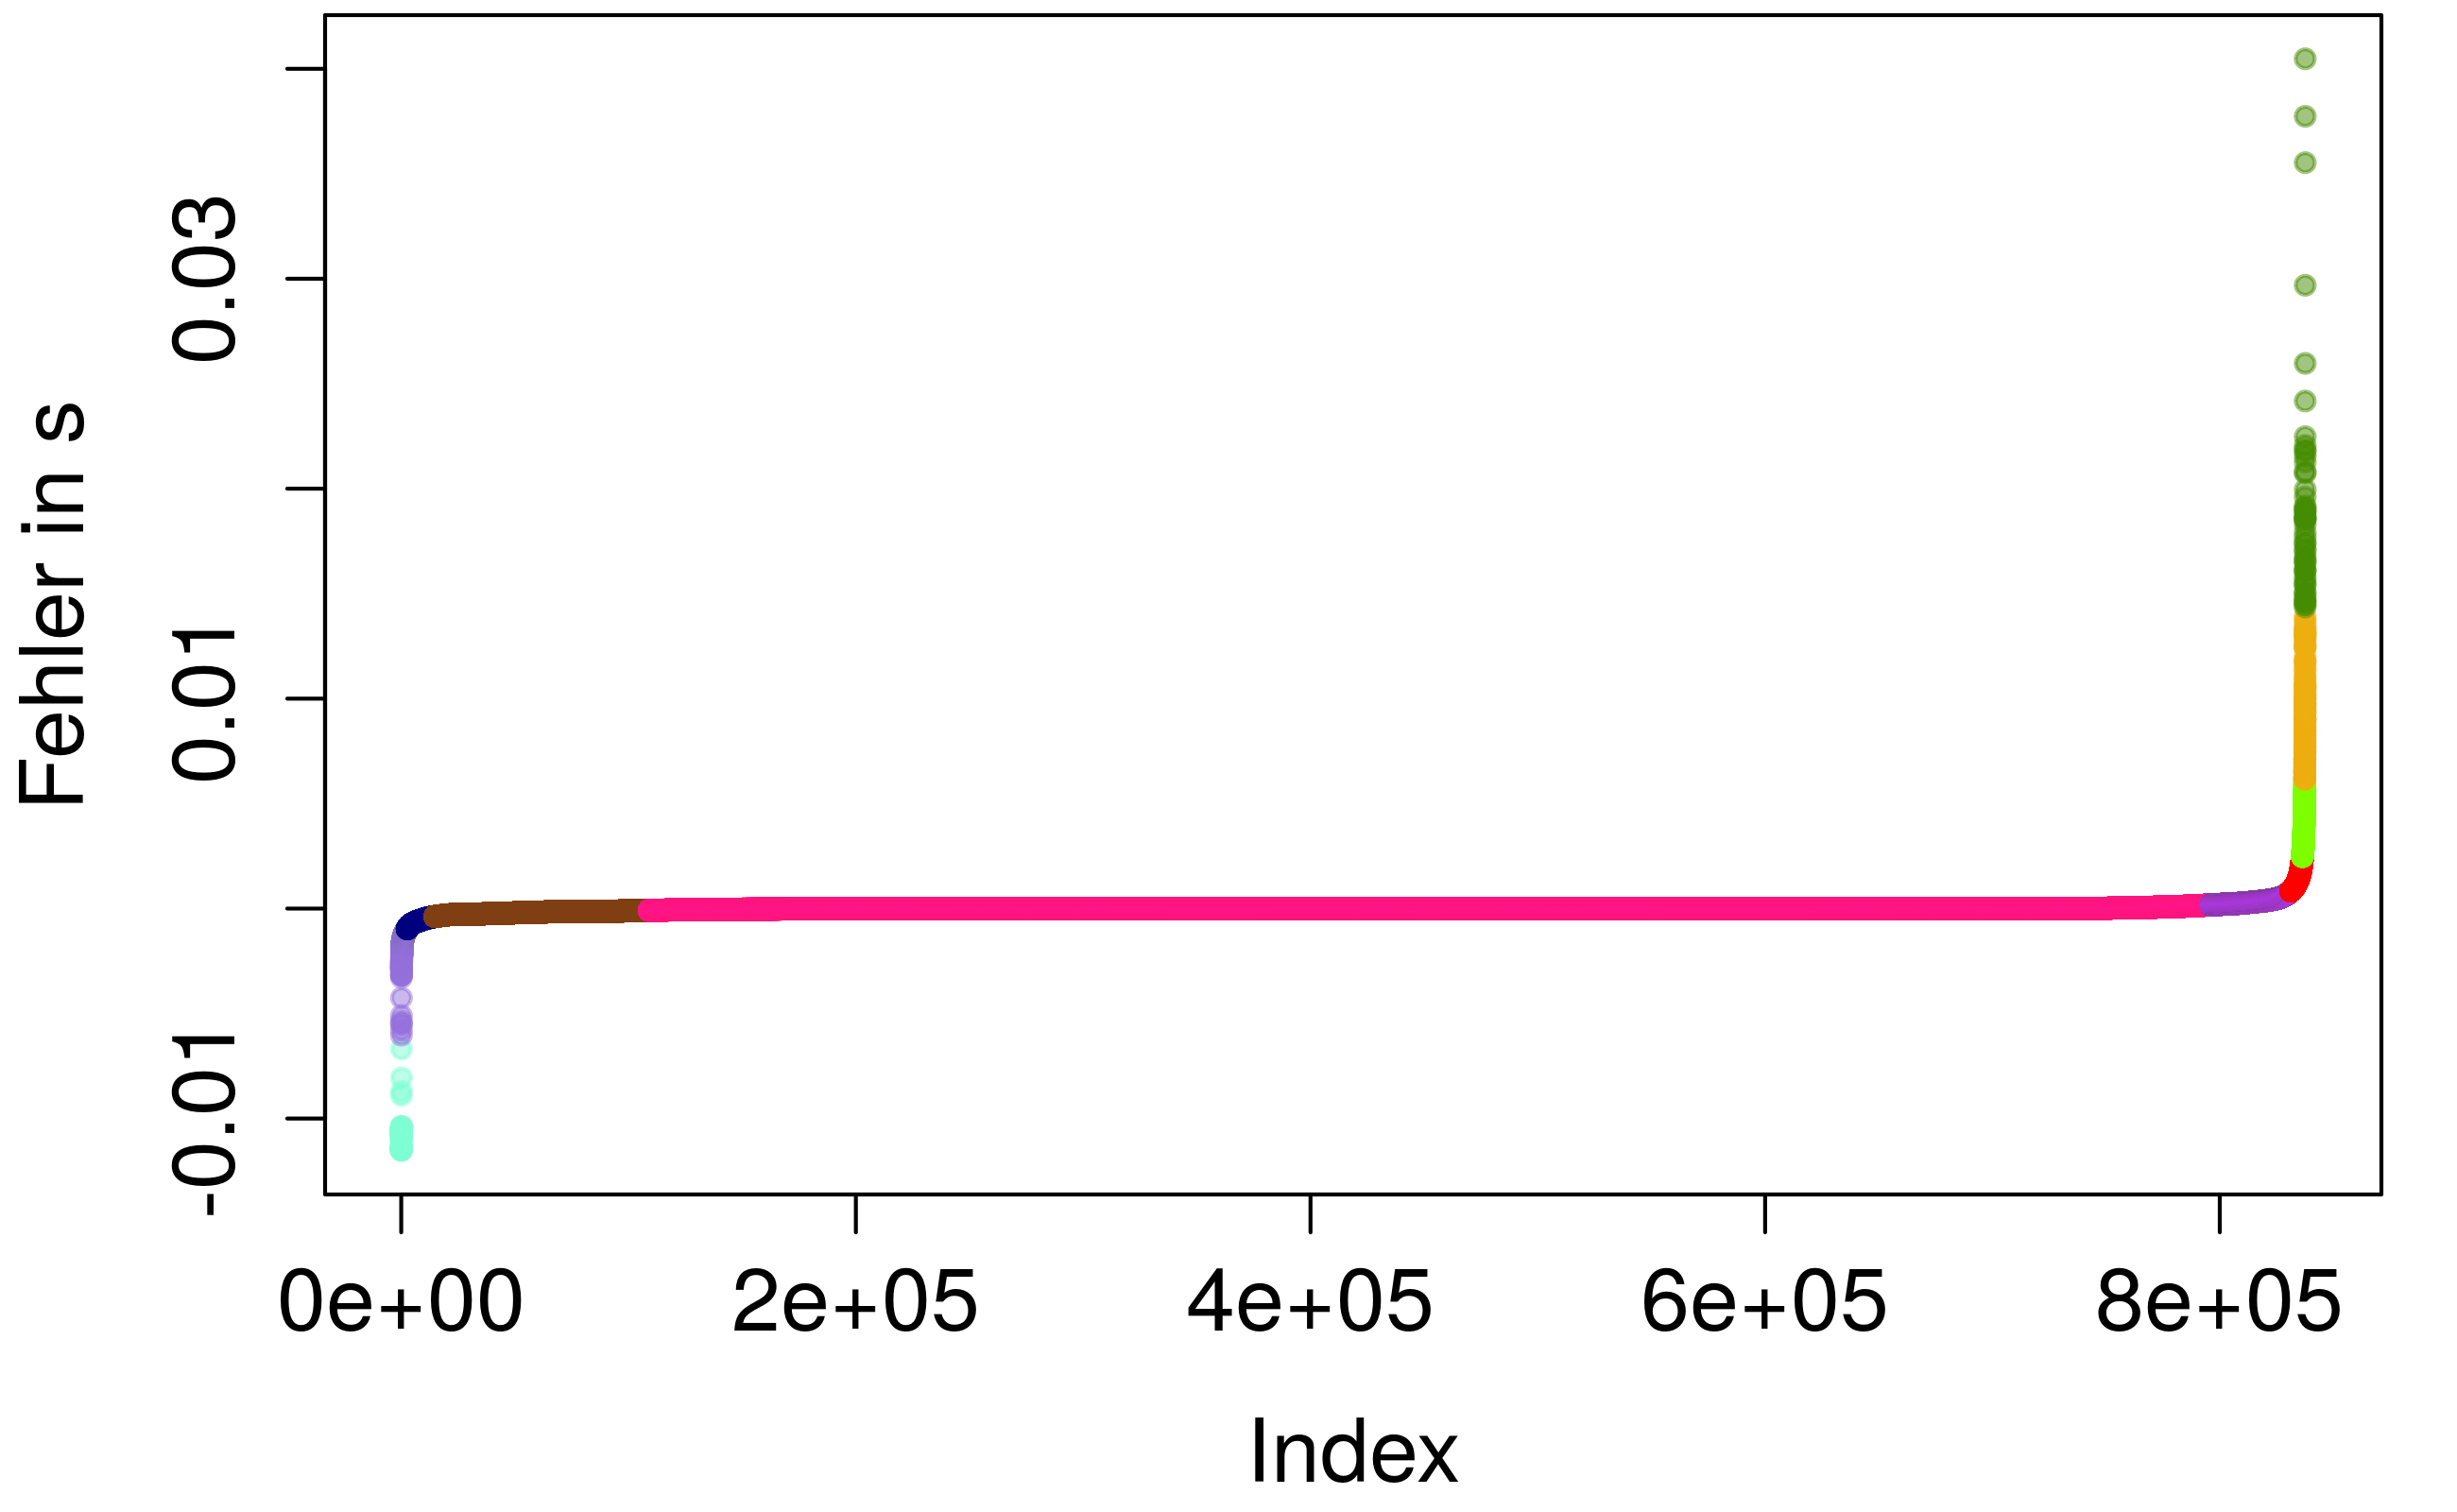
\includegraphics[width=1\linewidth]{Bilder/linreg_error_sorted_clustering_seq.png}
		\vspace*{-0.45cm}		
		\caption{sortierte Residuen}
		%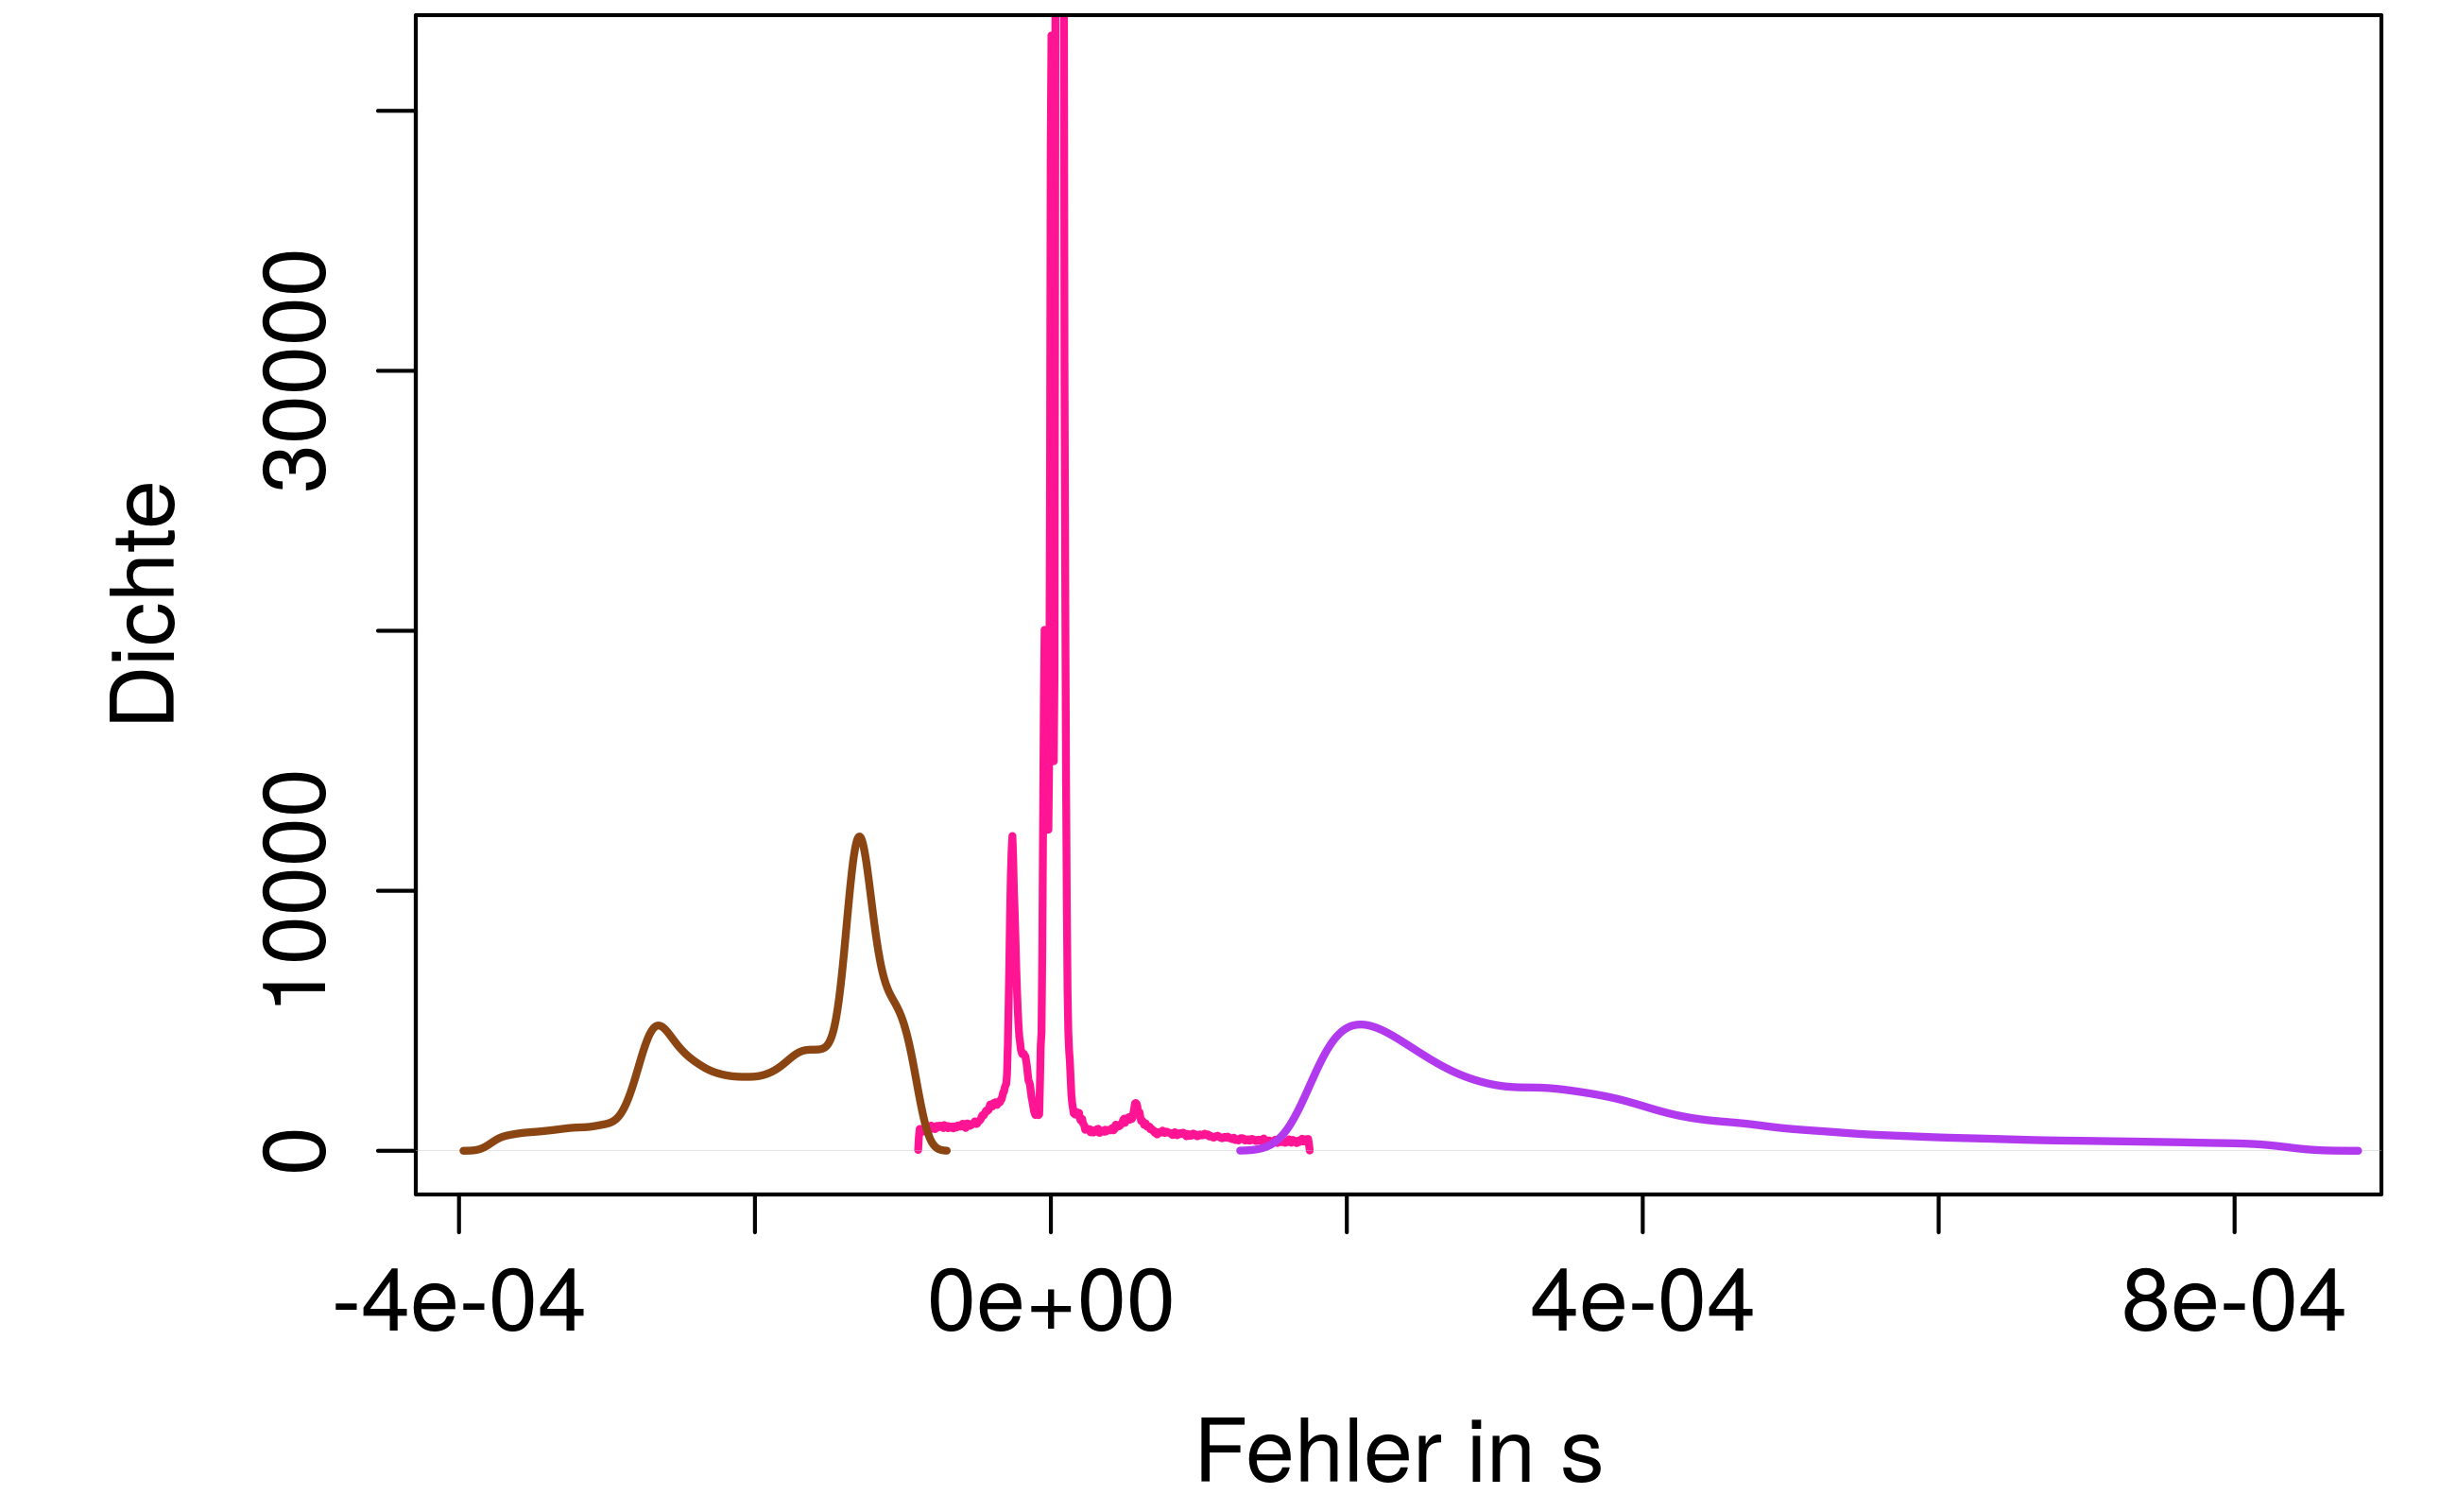
\includegraphics[width=1\linewidth]{Bilder/density_of_fk_seq.png}
		%Dichte, sollte eine klare Spitze pro Klasse aufweisen, dann korreliert die Fehlerklasse mit einem Pfad
		%\vspace*{-0.45cm}
		%\caption{Dichte der Klassen um den Nullpunkt}
	\end{figure}
\end{columns}
\end{frame}

\begin{frame}
\frametitle{Fehlerklassen auf RND}
\begin{columns}
\column{.45\textwidth}
	\begin{figure}
		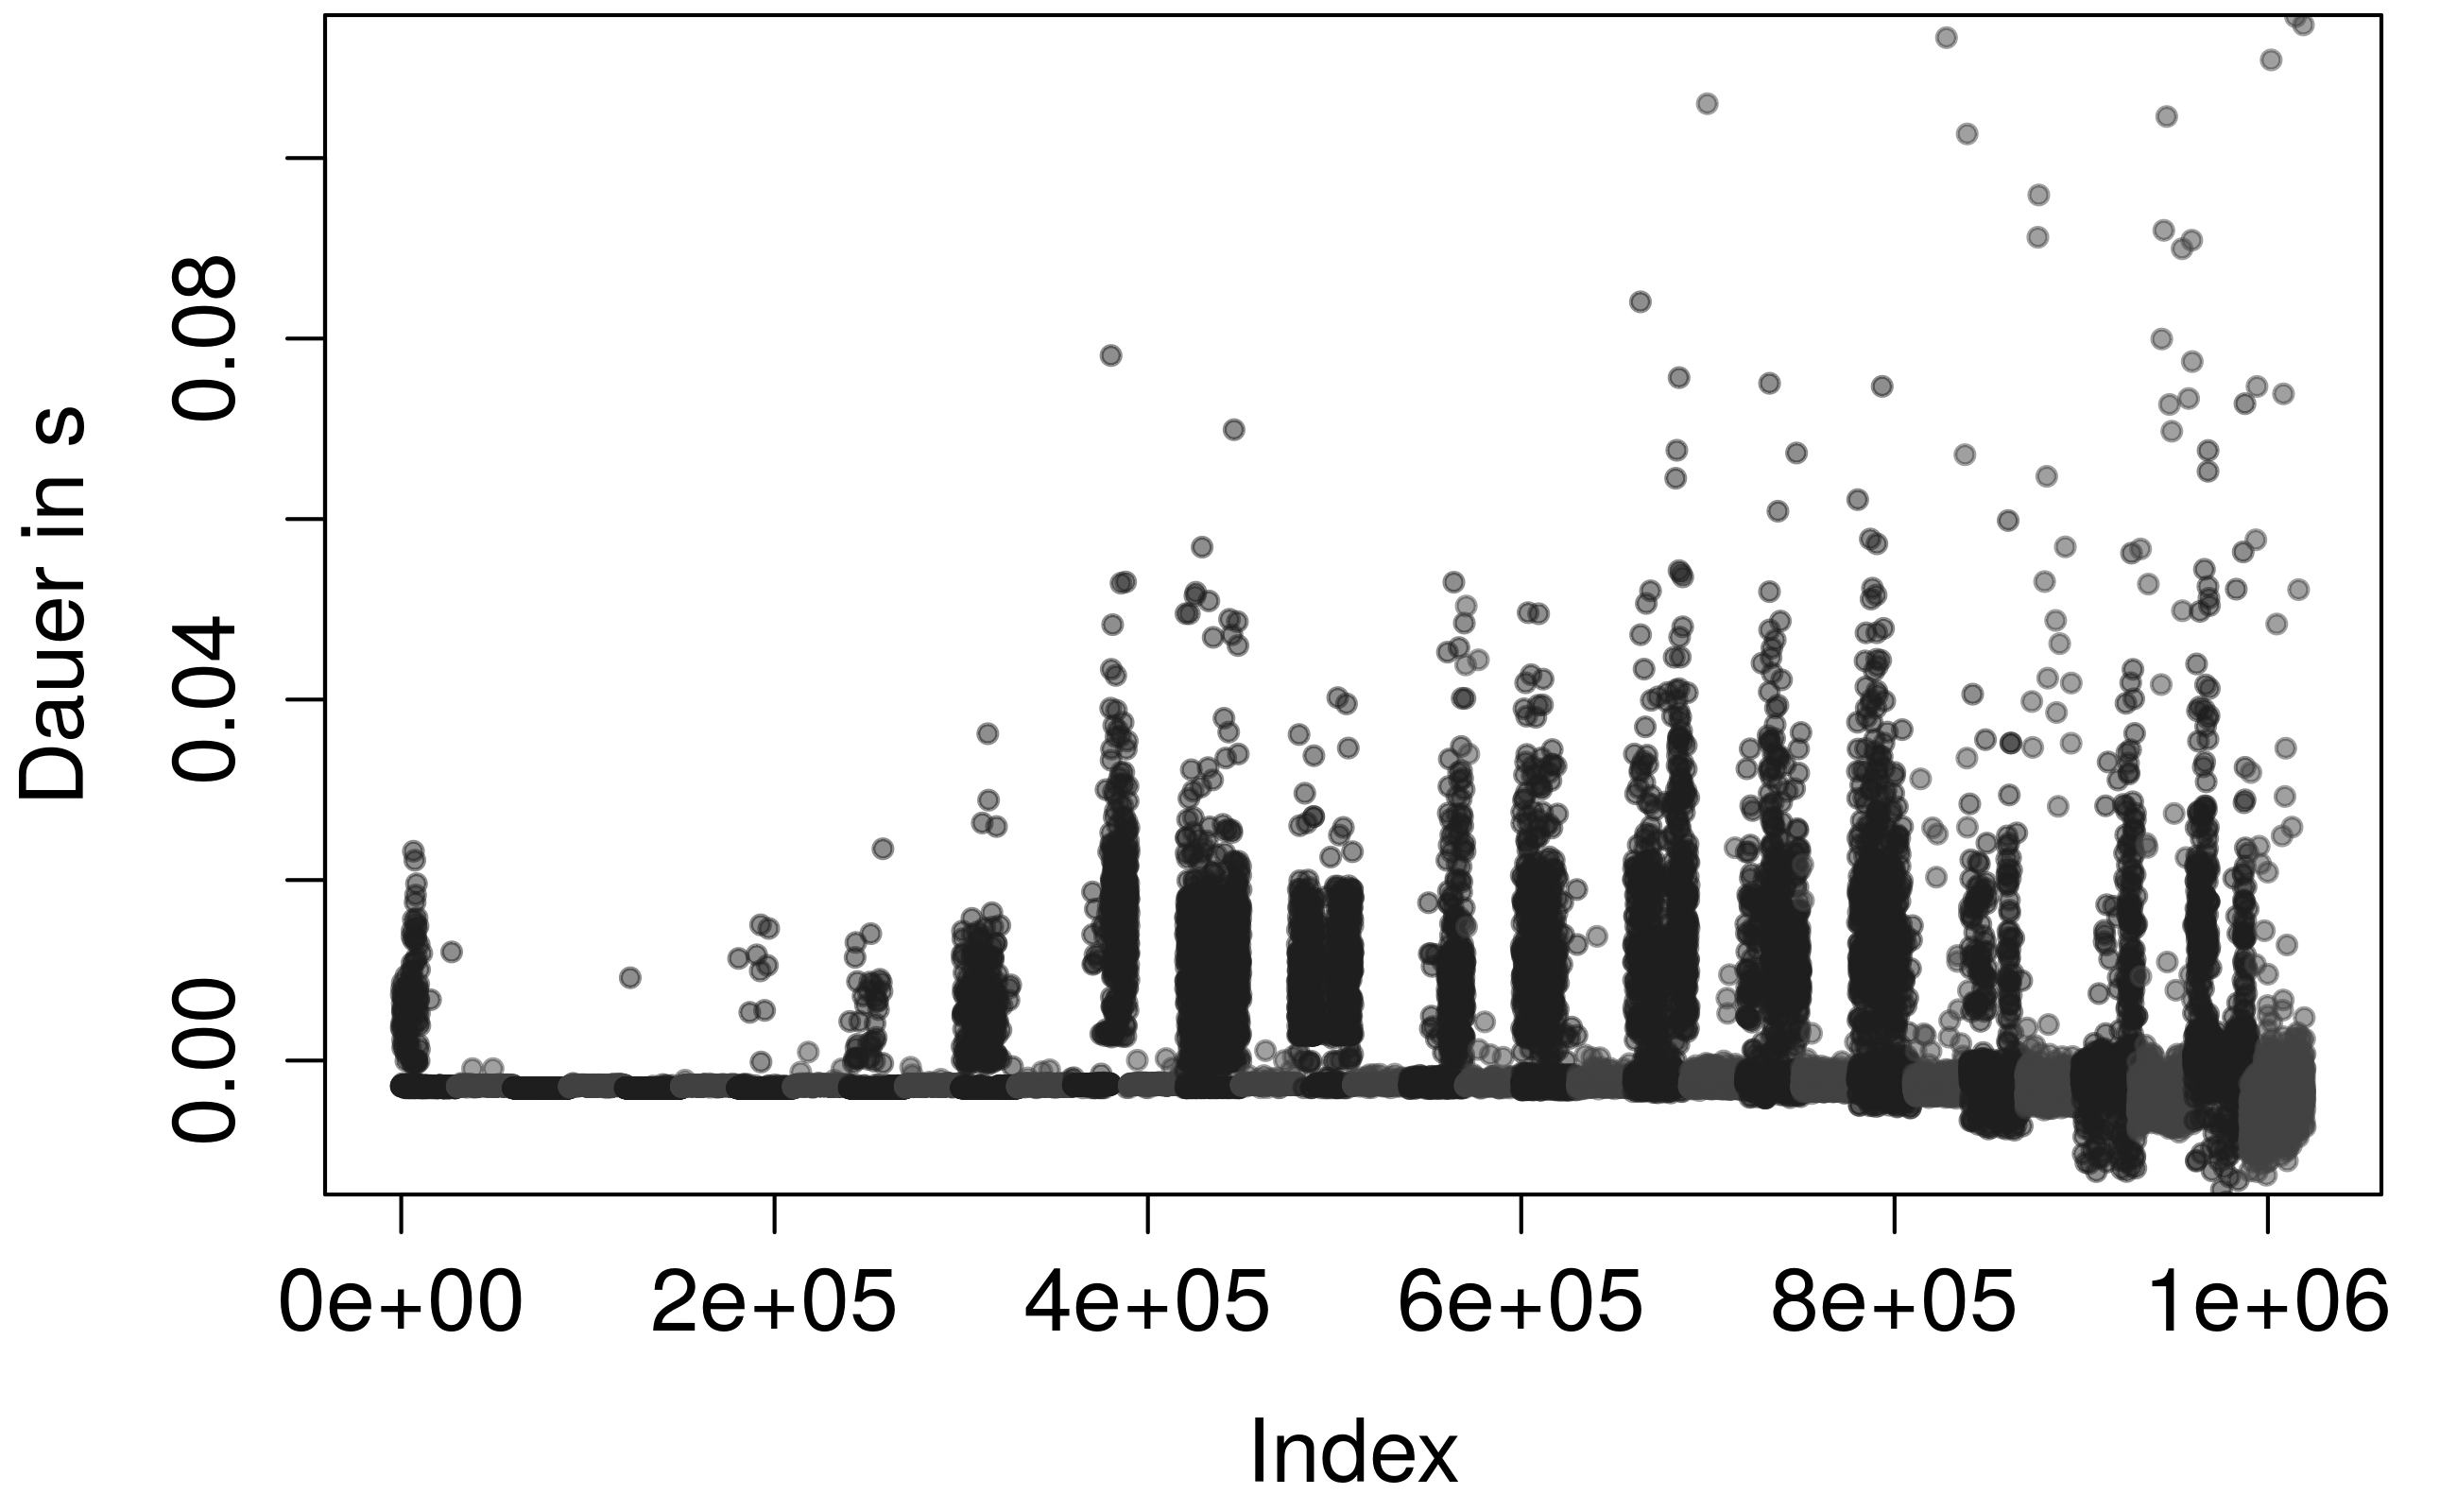
\includegraphics[width=1\linewidth]{Bilder/linreg_error_rnd_all.png}\\
		\vspace*{-0.45cm}
		\caption{Residuen von LinReg G auf RND}
		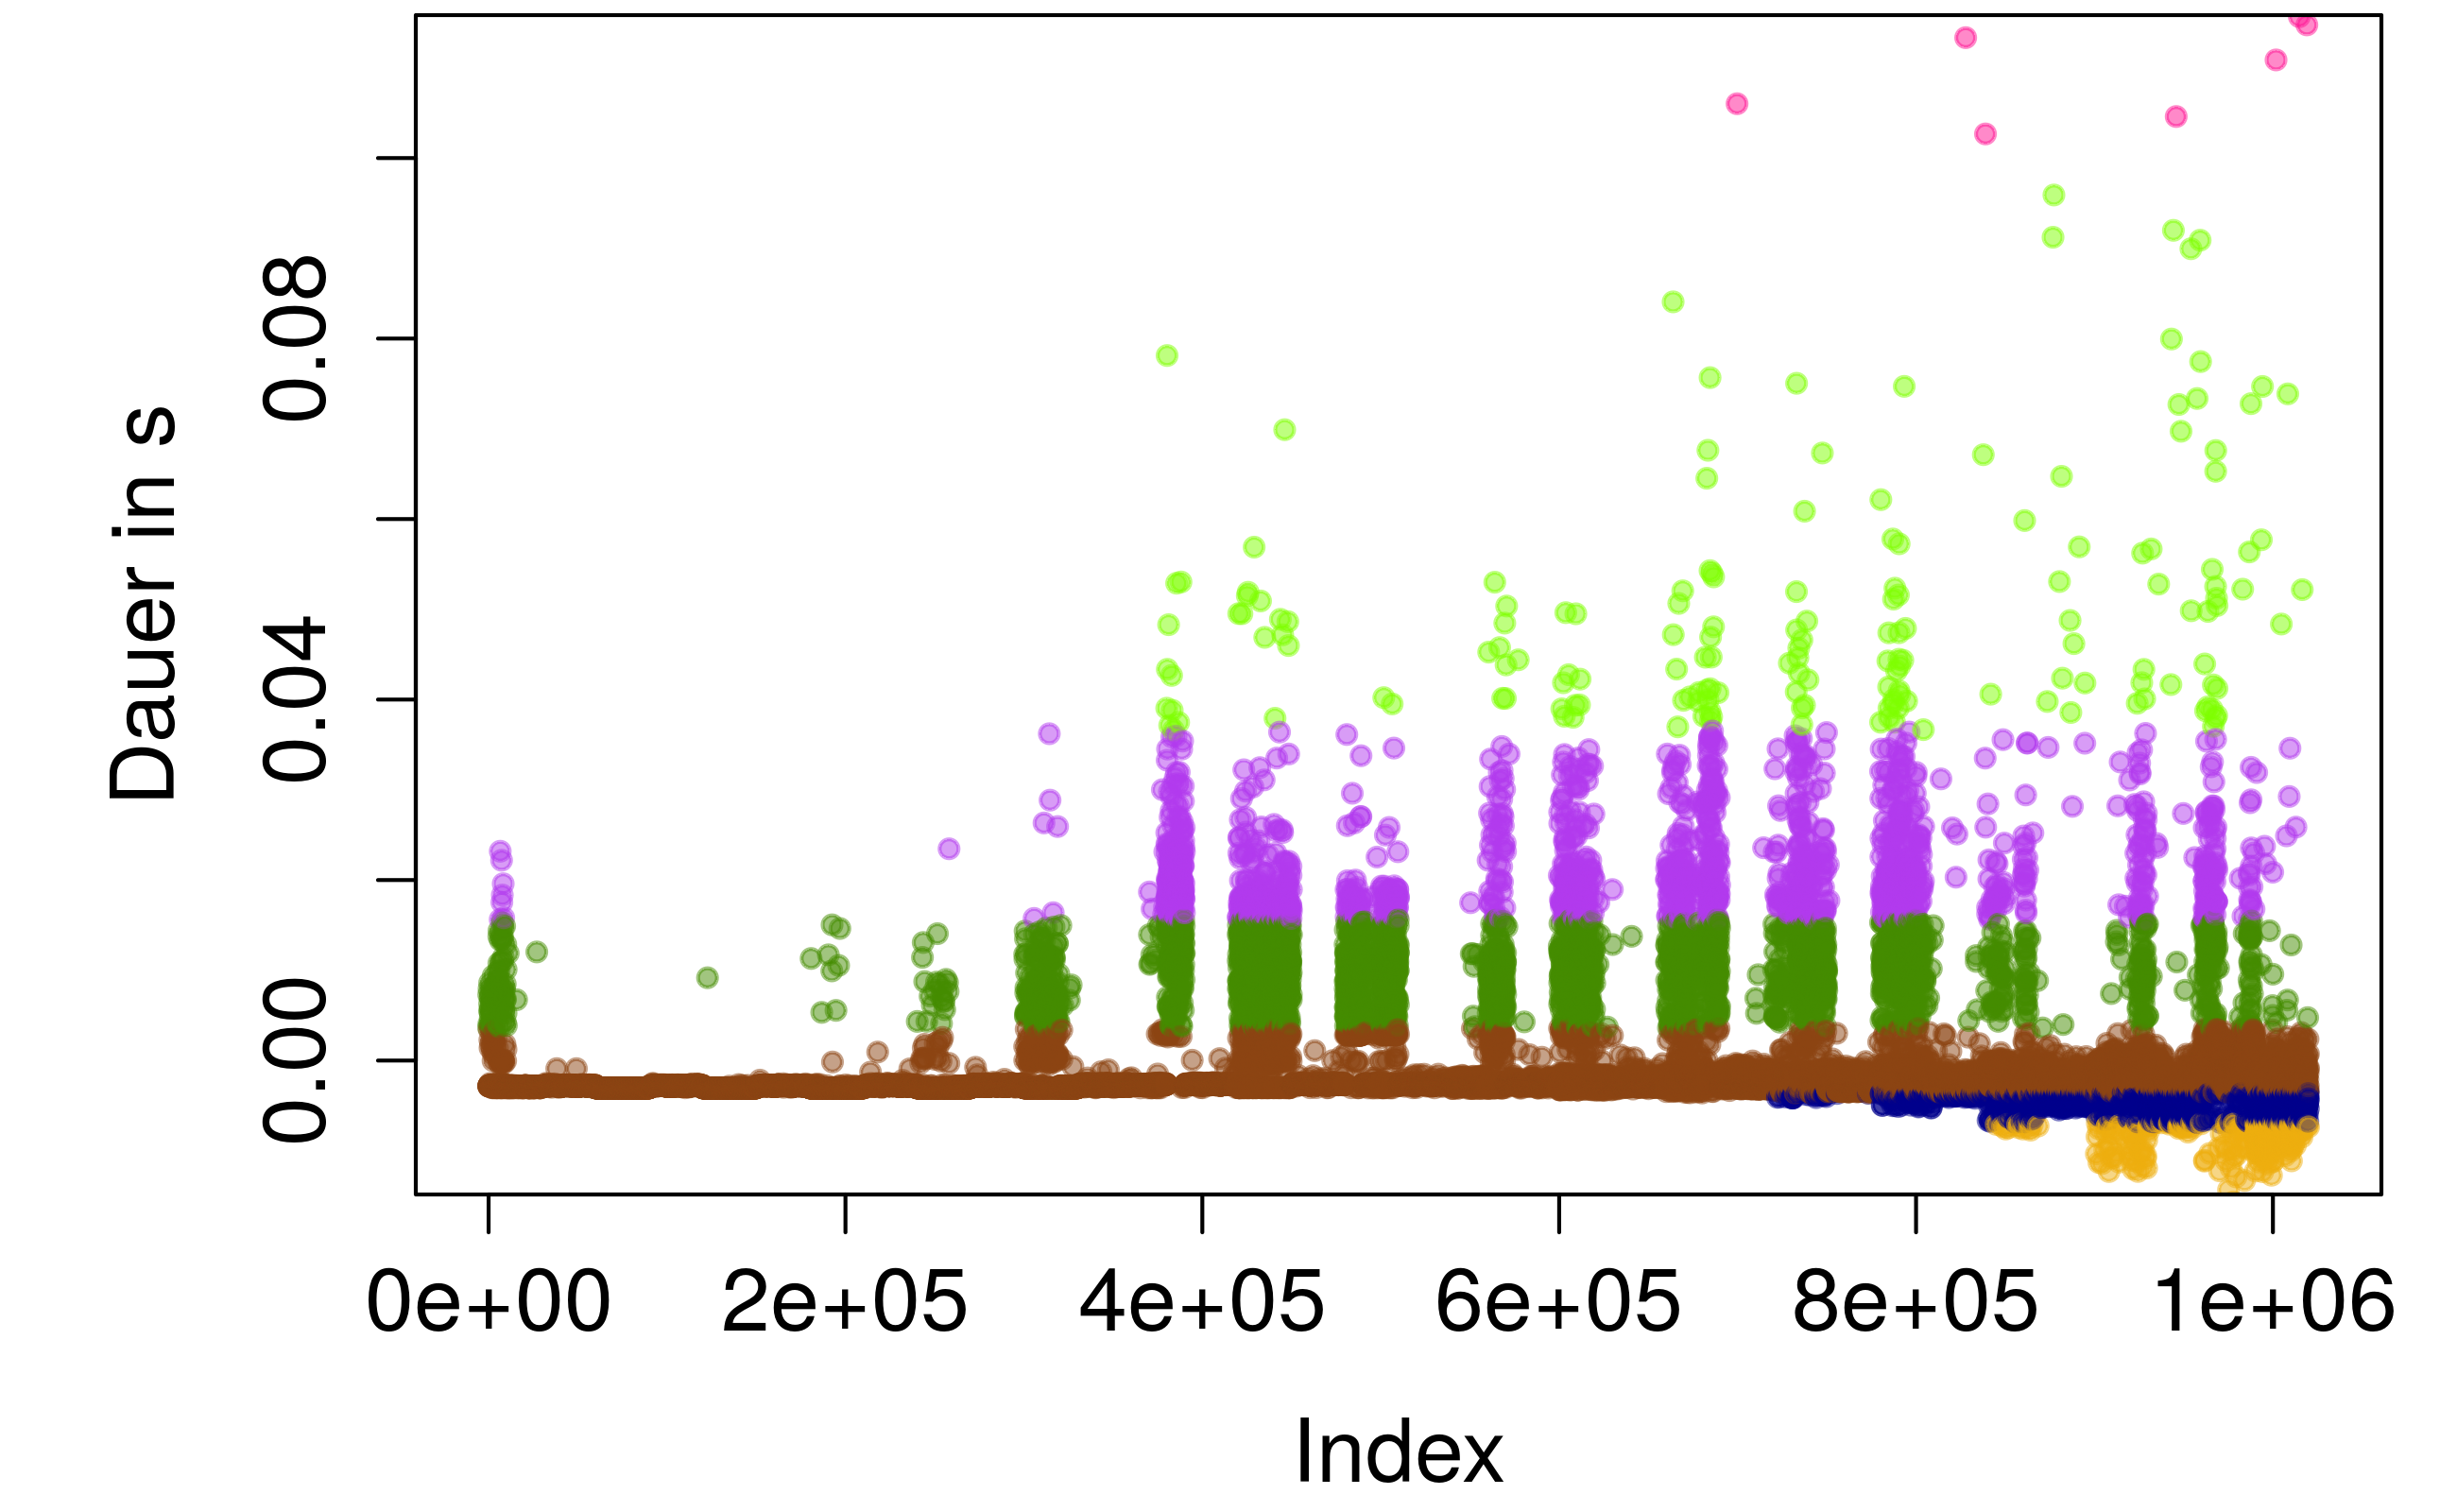
\includegraphics[width=1\linewidth]{Bilder/linreg_error_clustering_rnd_all.png}\\
		\vspace*{-0.45cm}
		\caption{Farblich markierte Fehlerklassen}
	\end{figure}
\column{.45\textwidth}
	\begin{figure}
		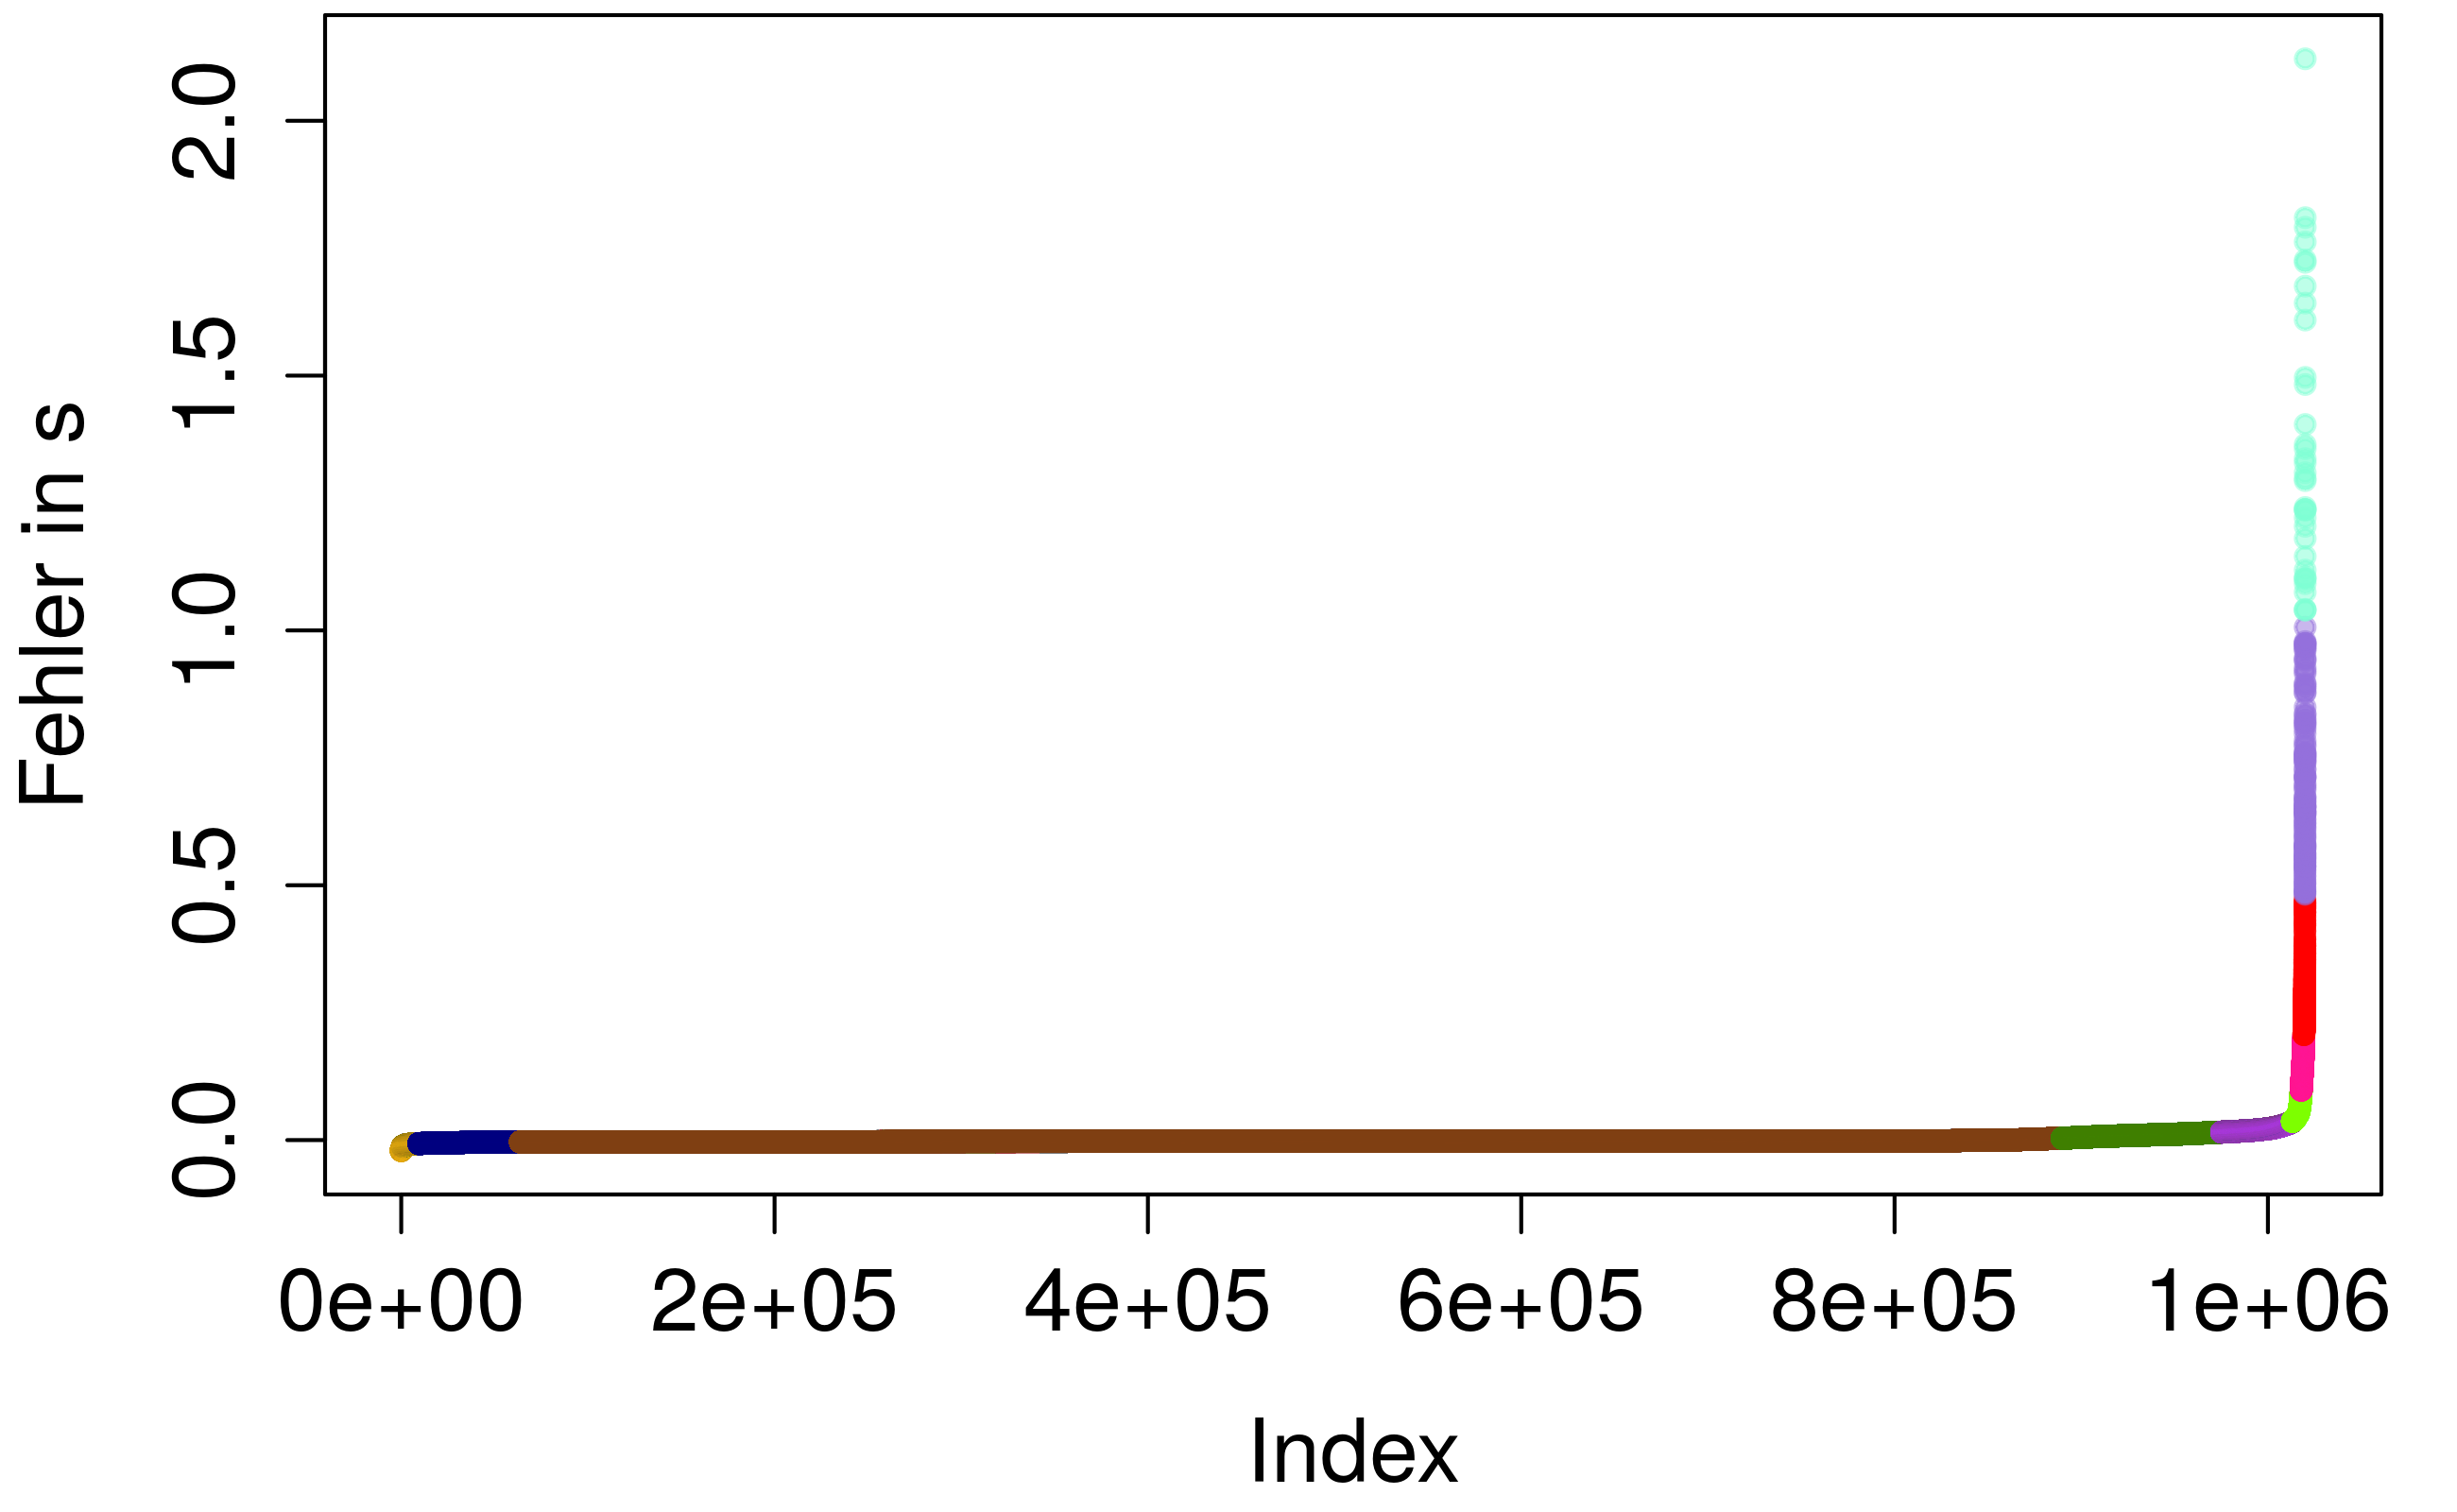
\includegraphics[width=1\linewidth]{Bilder/linreg_error_sorted_clustering_rnd.png}
		\vspace*{-0.45cm}
		\caption{sortierte Residuen}
		%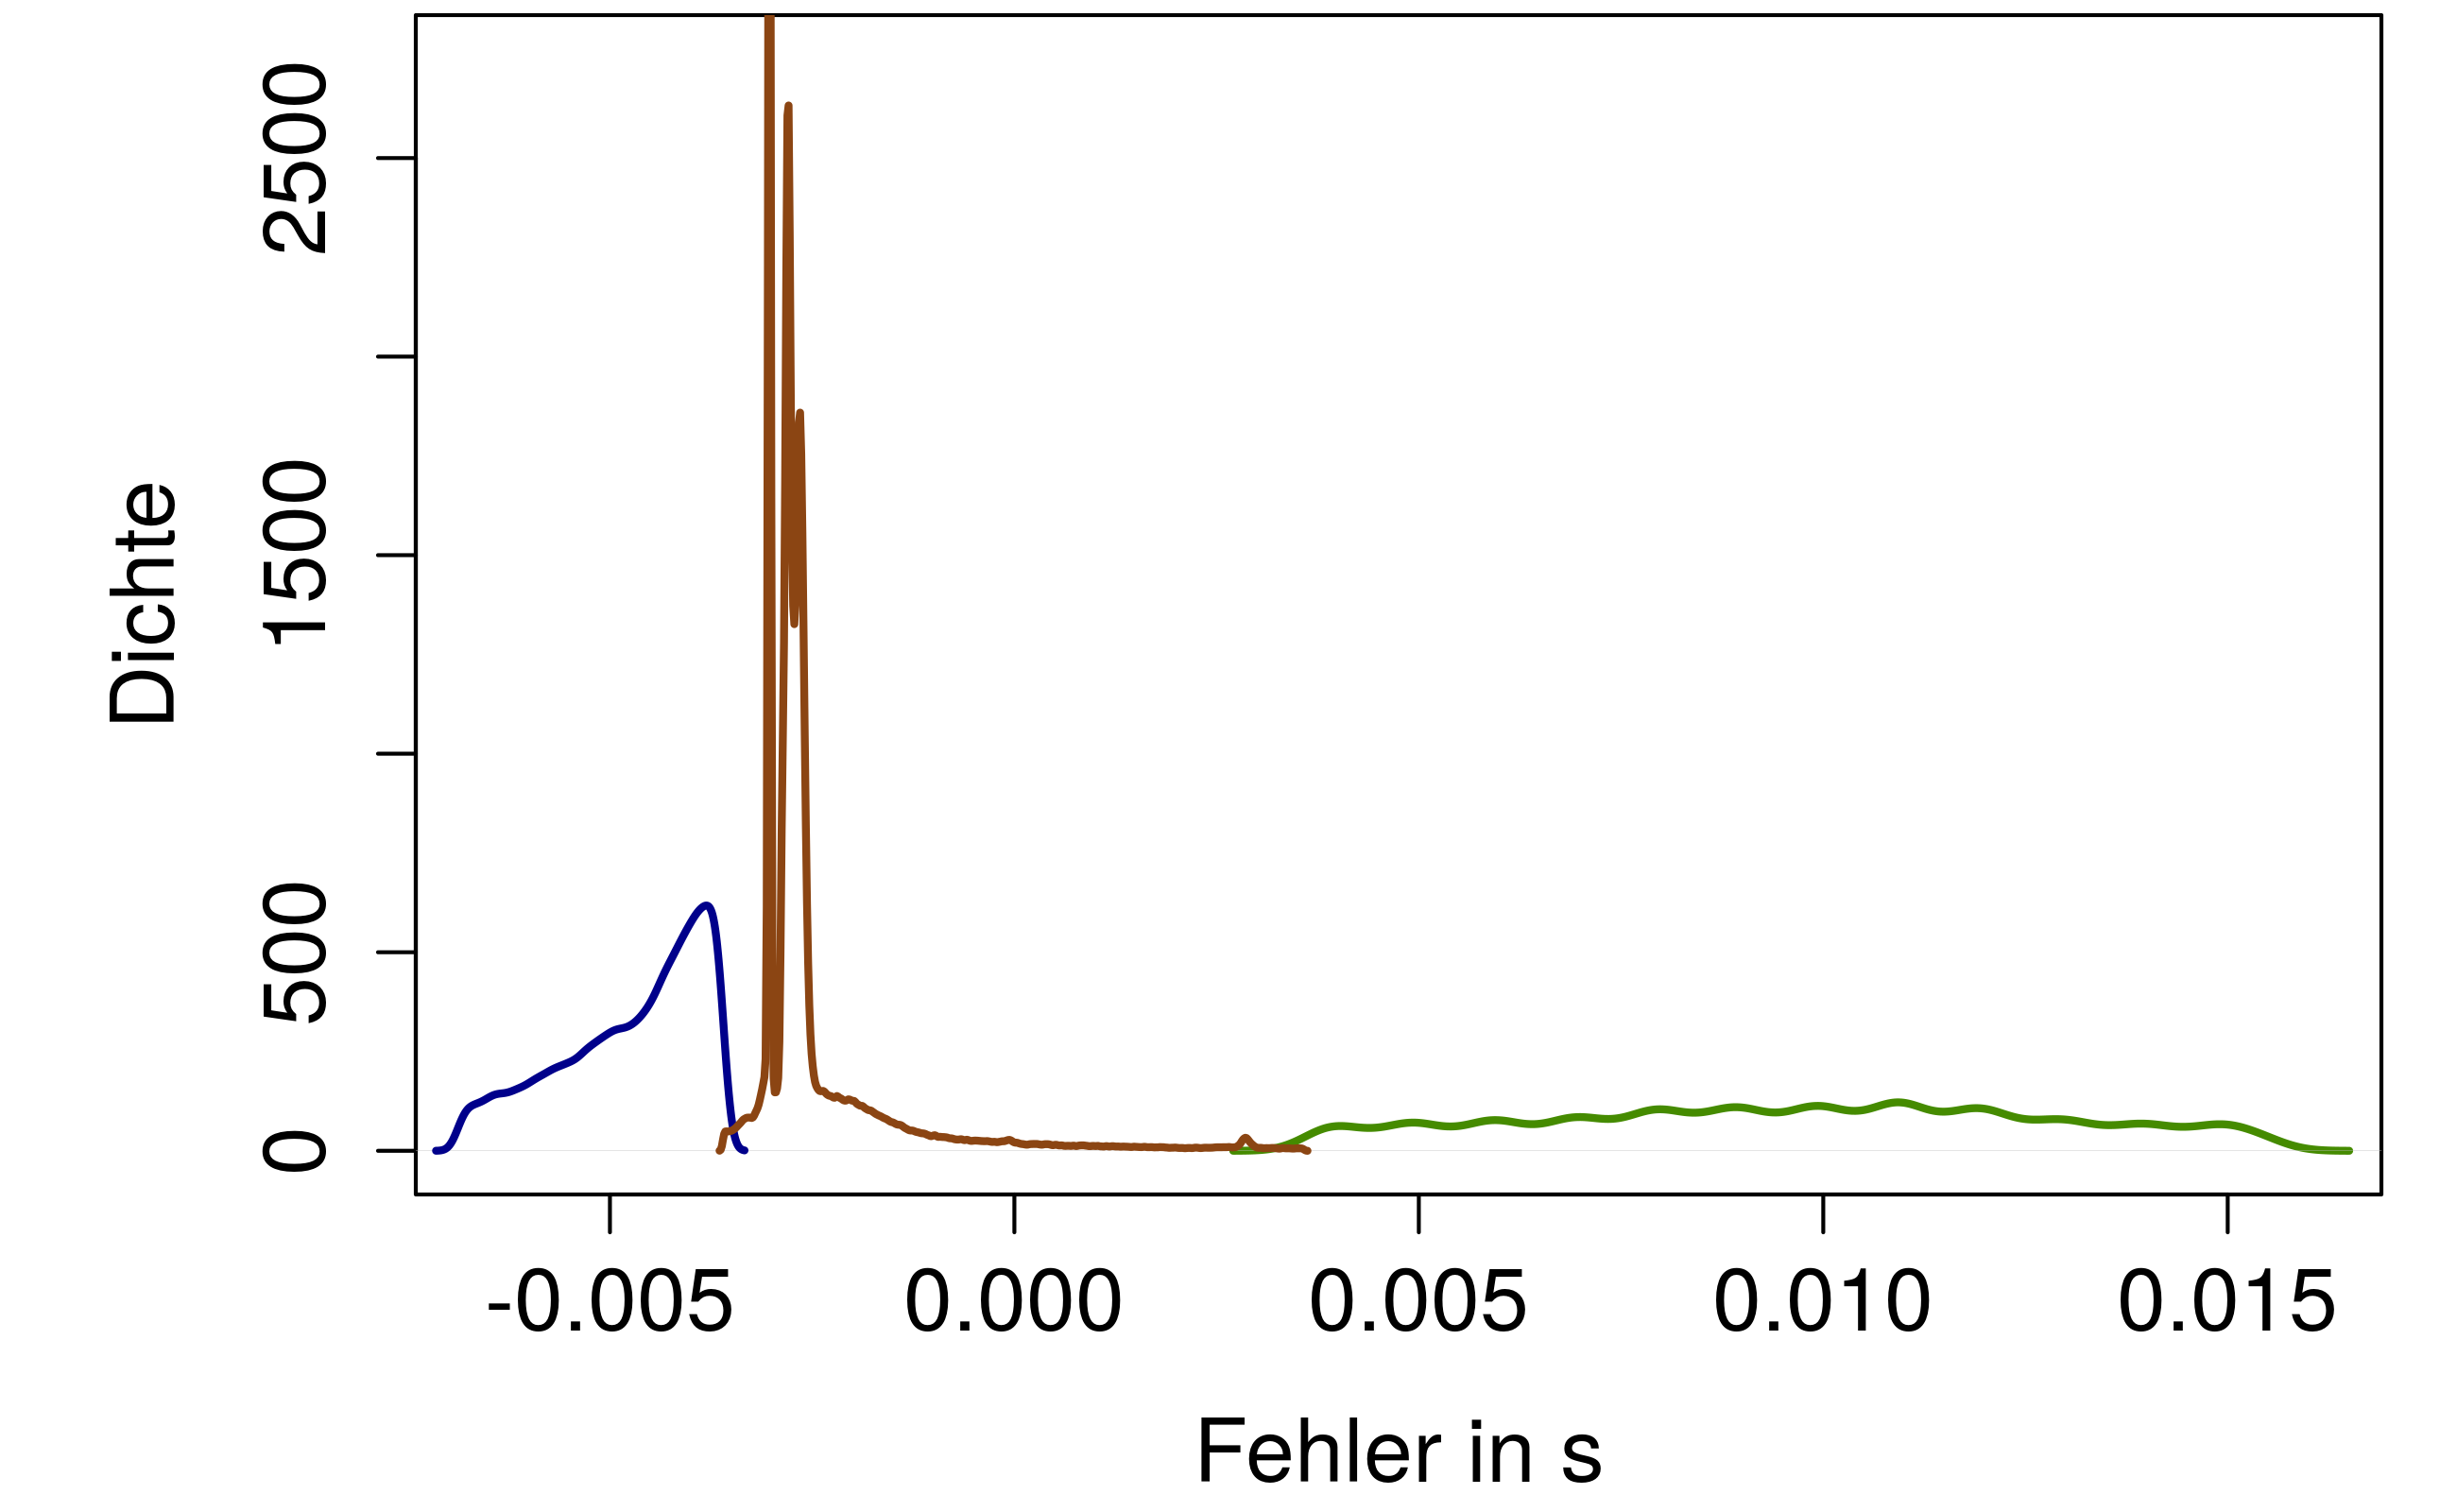
\includegraphics[width=1\linewidth]{Bilder/density_of_fk_rnd.png}
		%\vspace*{-0.45cm}
		%\caption{Dichte der Klassen um den Nullpunkt}
	\end{figure}
\end{columns}
\end{frame}

\subsection{Ergebnisse von Modellen mit Fehlerklassen}
\begin{frame}
	\frametitle{Modell mit Fehlerklassen}
	\begin{columns}
		\column{.55\textwidth}
		\begin{itemize}
			\item<1-> Durchschnittliche Zugriffszeit (\textbf{Durchschnitt})
			\item<1-> Lineare Regression nach der Zugriffsgröße (\textbf{LinReg G})
			%nach weiteren Attributen als nicht besser herausgestellt
			\item<1-> Einfaches Modell mit neuronalem Netz (\textbf{NN-Tupel1})
			%Zugriffsgröße, DeltaOffset, OpTyp auf Zugriffszeit
			\item<1-> Ausnutzen zeitlicher Abhängigkeit mit dem \textit{exponential moving average}(\textbf{NN-EMA})
			%ema, exponential moving average
			%2 BILDER erstellen! einmal attribute zu zugriffsdauer und einmal beispiel von ema
		\end{itemize}
		\column{.6\textwidth}
		\begin{figure}
			\includegraphics<1->[width=1\linewidth]{Dot/linregfk.png}
		\end{figure}
	\end{columns}
\end{frame}






\begin{frame}
\frametitle{Modell mit Fehlerklassen auf SEQ}
\begin{table}
	\resizebox{\textwidth}{!}{
		\begin{tabular}{|p{2.5cm}|r|r|r|r|r|}\hline%
				Modell & MAE\,(s) &  MAPE\,(\%) & MSPE\,(\%) & RMax\,(\%) \\\hline\hline
				\csvreader[late after line=\\\hline]%
				{CSV/latex_seq_results_fk.csv}{Modell=\Model,MAF=\MAF,RMAF=\RMAF, RMQA = \RMQA, Q3 = \Q3, Max = \Max,RMAFTraining = \RMAFTraining, Bereich = \Bereich, RMAFavg = \RMAFavg}%
				{\Model & \MAF & \RMAF & \RMQA & \Max}%
		\end{tabular}
	}
\end{table}
\begin{itemize}
\item MAE: \textit{mean absolute error}
\item MAPE: \textit{mean absolute percentage error}
\item MSPE: \textit{mean square percentage error}
%\item RQ3: drittes Quartil aller relativen Modellabweichungen
\item RMax: maximale relative Modellabweichung
\end{itemize}
\end{frame}

\begin{frame}
\frametitle{Modell mit Fehlerklassen auf RND}
\begin{table}
	\resizebox{\textwidth}{!}{
		\begin{tabular}{|p{2.5cm}|r|r|r|r|r|}\hline%
				Modell & MAE\,(s) & MAPE\,(\%) & MSPE\,(\%) & RMax\,(\%) \\\hline\hline
			\csvreader[late after line=\\\hline]%
				{CSV/latex_rnd_results_fk.csv}{Modell=\Model,MAF=\MAF,RMAF=\RMAF, RMQA = \RMQA, Q3 = \Q3, Max = \Max,RMAFTraining = \RMAFTraining, Bereich = \Bereich, RMAFavg = \RMAFavg}%
				{\Model & \MAF & \RMAF & \RMQA & \Max}%
		\end{tabular}
	}
\end{table}
\begin{itemize}
\item MAE: \textit{mean absolute error}
\item MAPE: \textit{mean absolute percentage error}
\item MSPE: \textit{mean square percentage error}
%\item RQ3: drittes Quartil aller relativen Modellabweichungen
\item RMax: maximale relative Modellabweichung
\end{itemize}
\end{frame}

\begin{frame}
\frametitle{Mit und ohne Fehlerklassen}
\begin{columns}
\column{.45\textwidth}
	\begin{figure}
		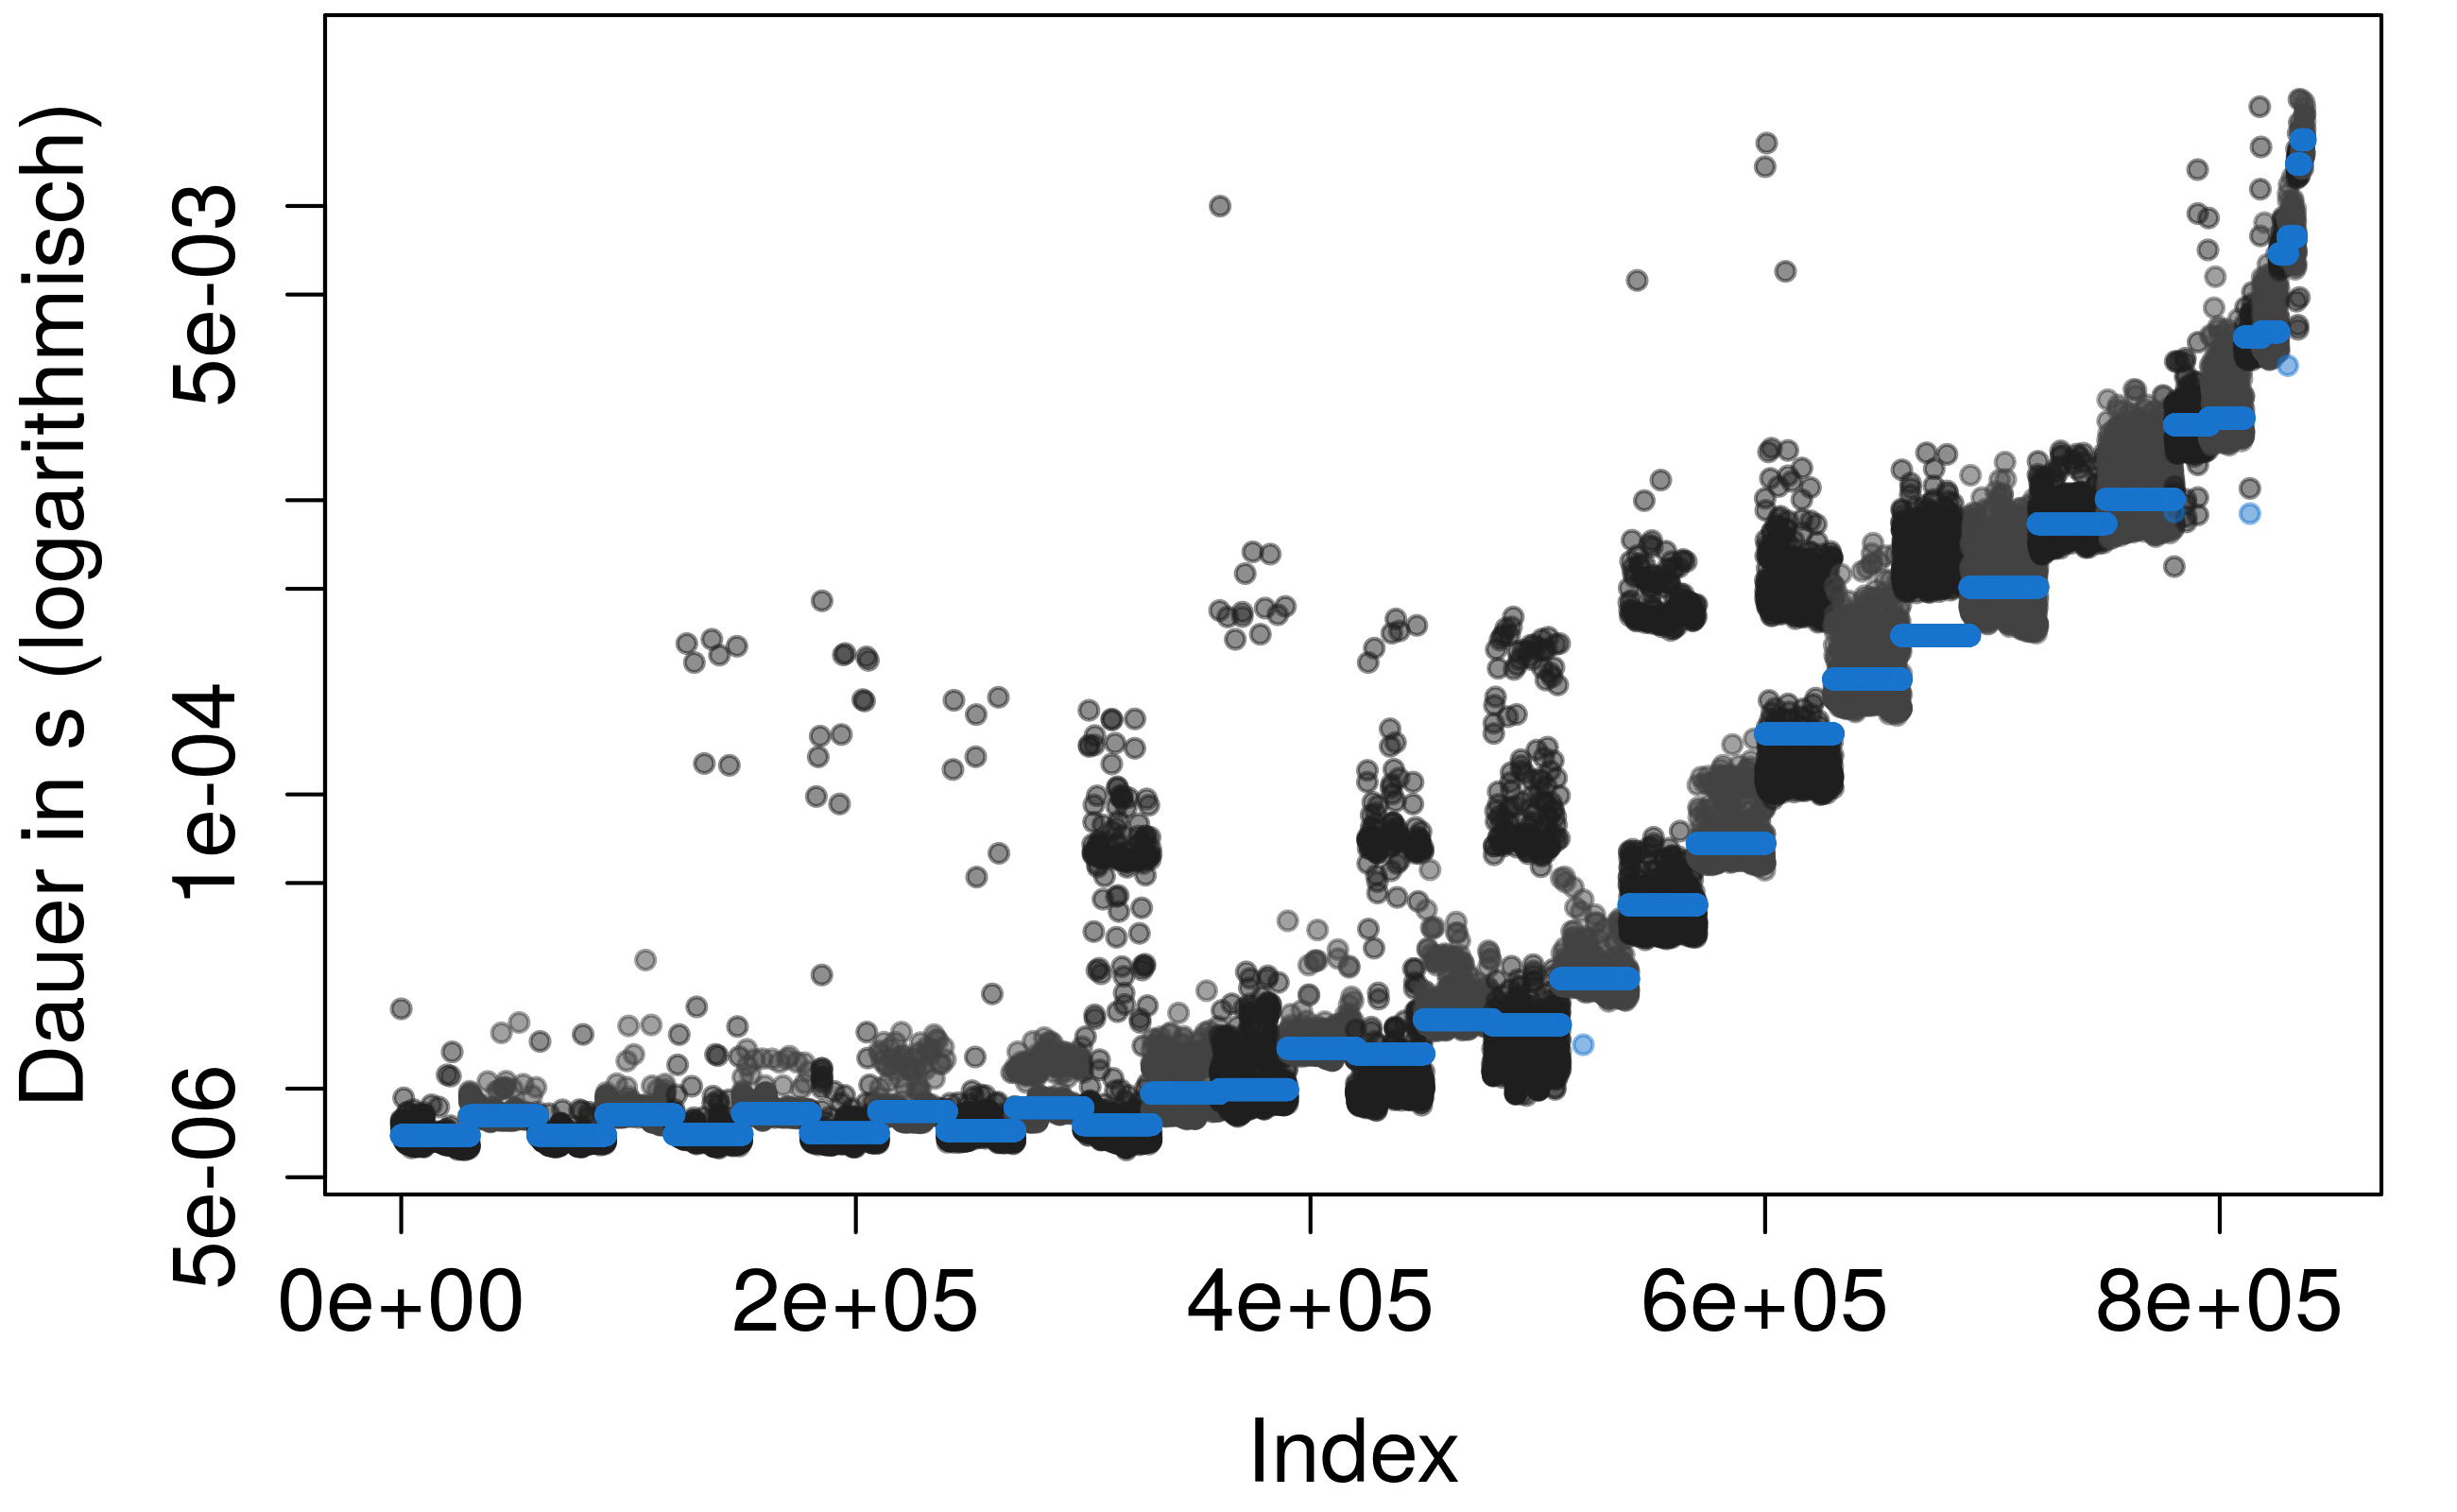
\includegraphics[width=1\linewidth]{Bilder/plot_onlyPred_tuple1_Duration_seq.png}\\
		\vspace*{-0.45cm}
		\caption{NN-Tupel1 auf SEQ}
		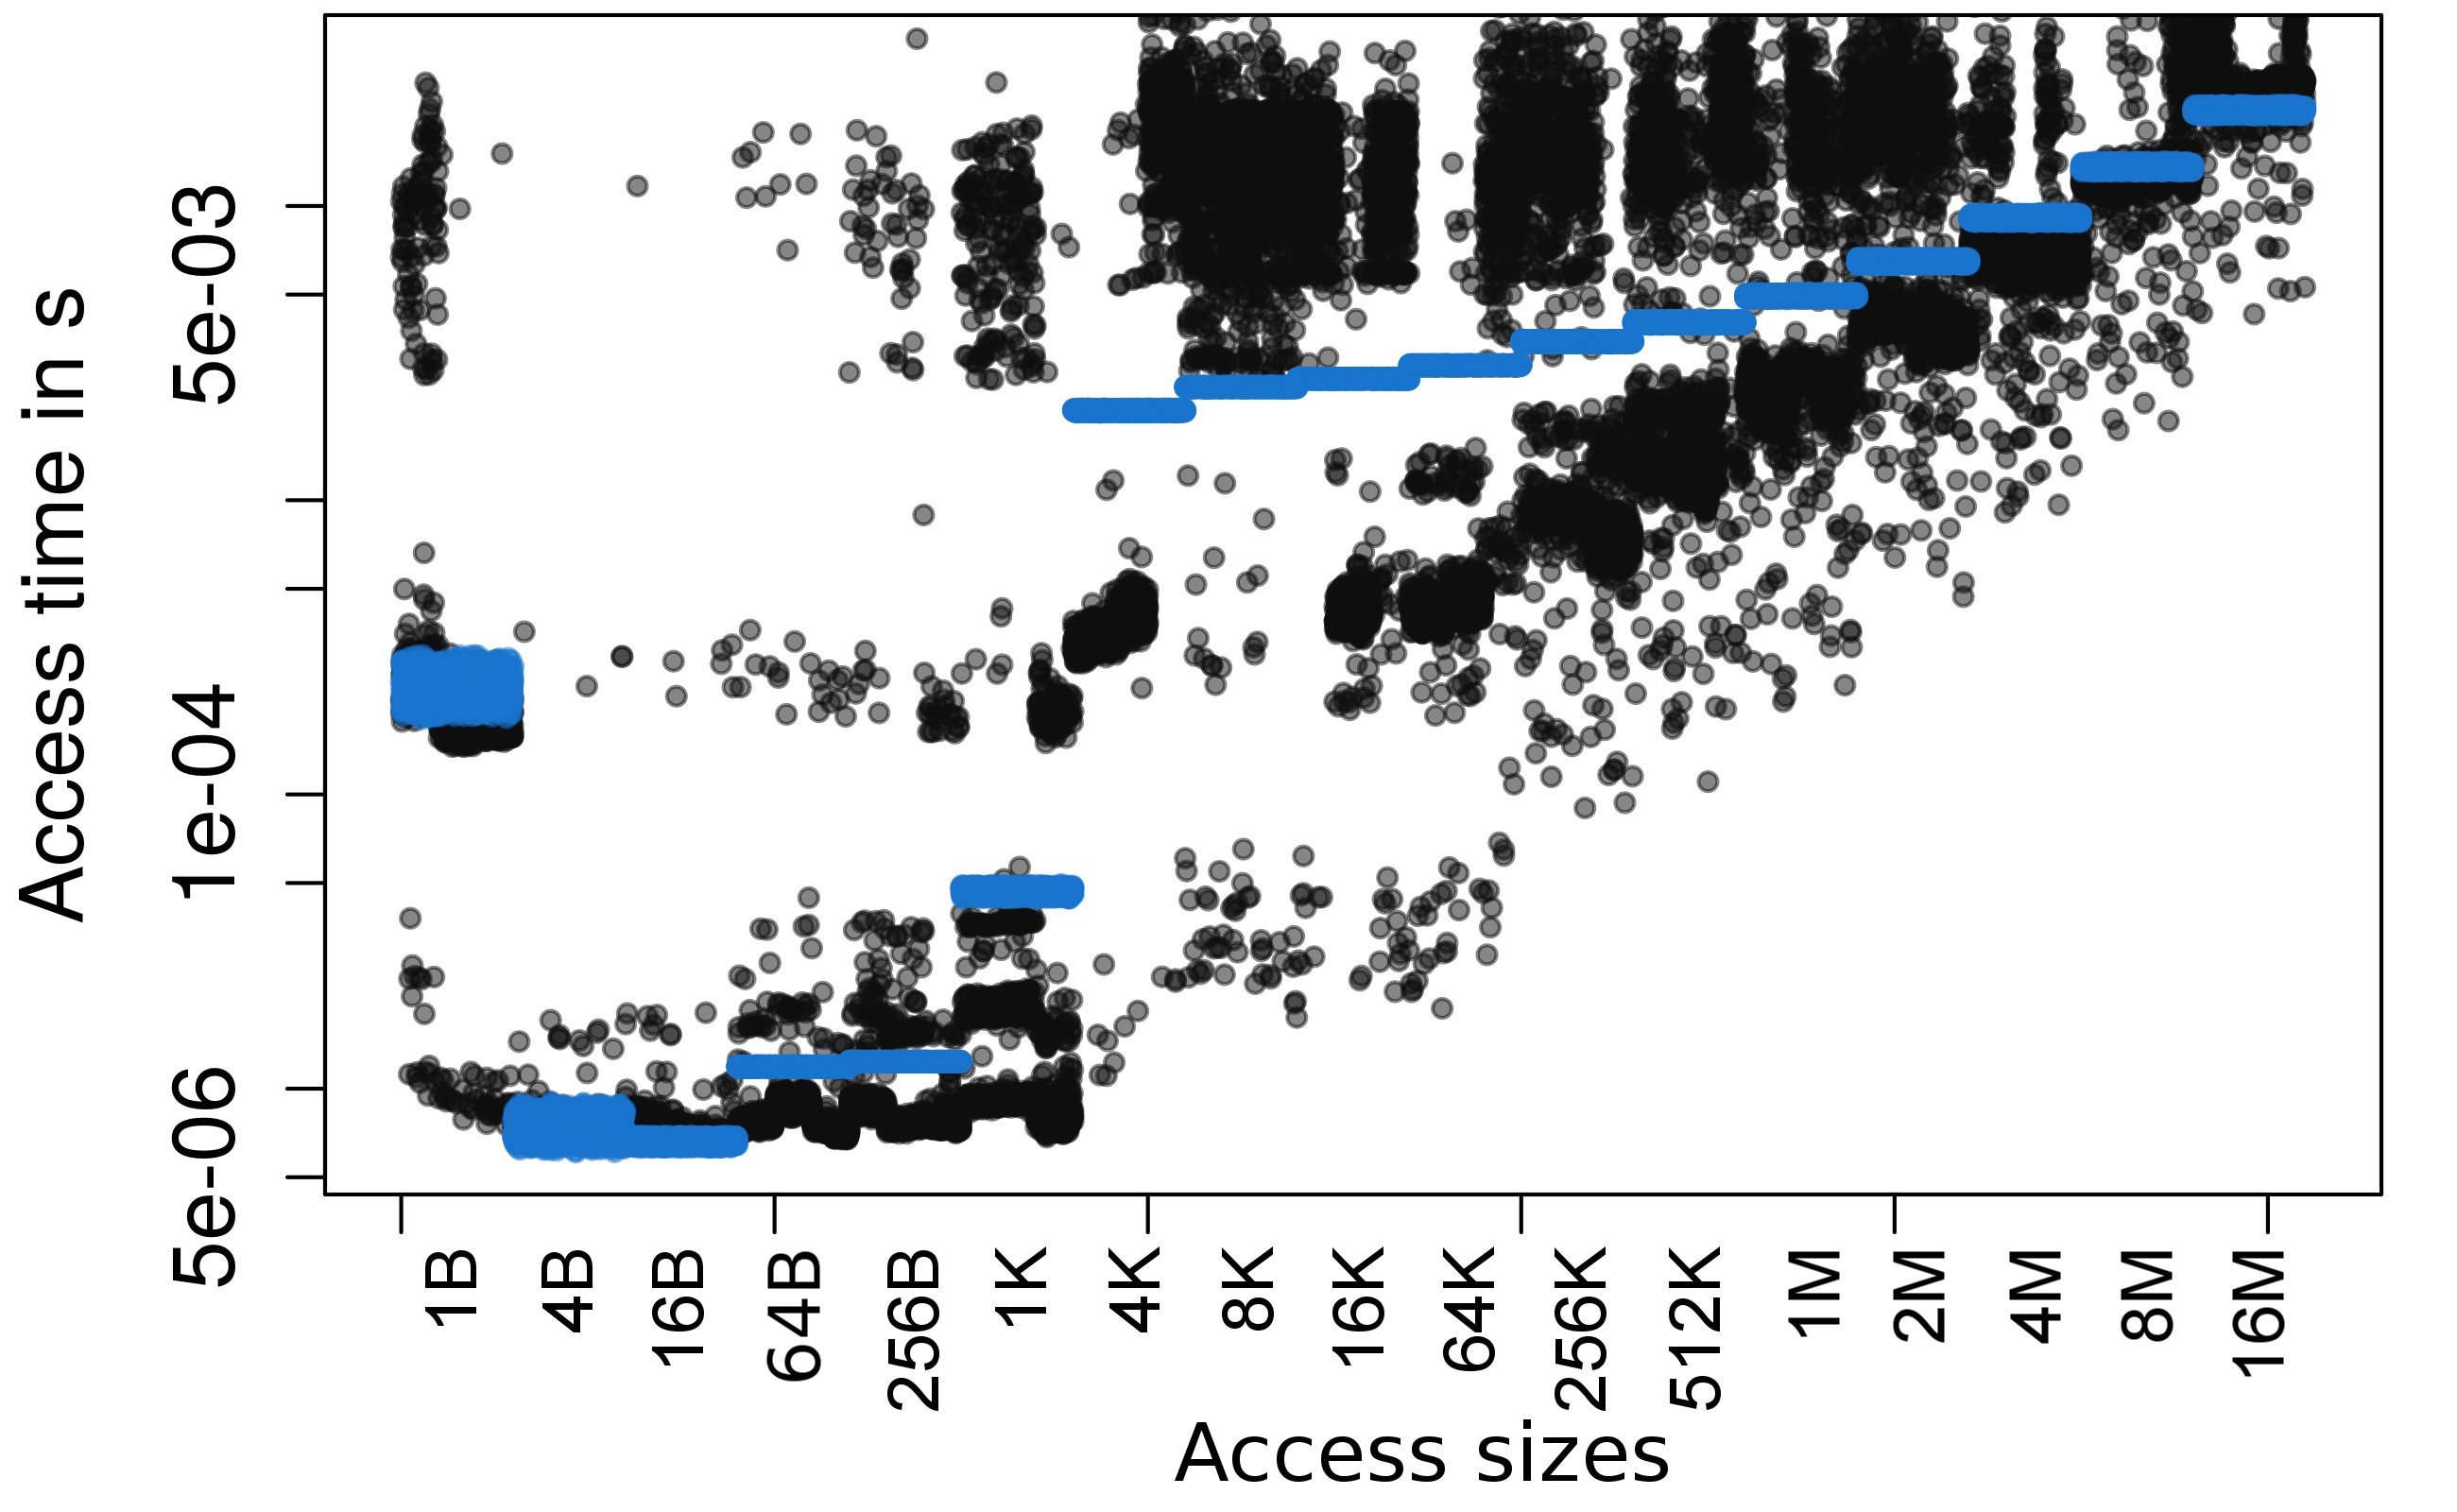
\includegraphics[width=1\linewidth]{Bilder/plot_onlyPred_tuple1_Duration_rnd.png}
		\vspace*{-0.45cm}
		\caption{NN-Tupel1 auf RND}
	\end{figure}
\column{.45\textwidth}
		\begin{figure}
		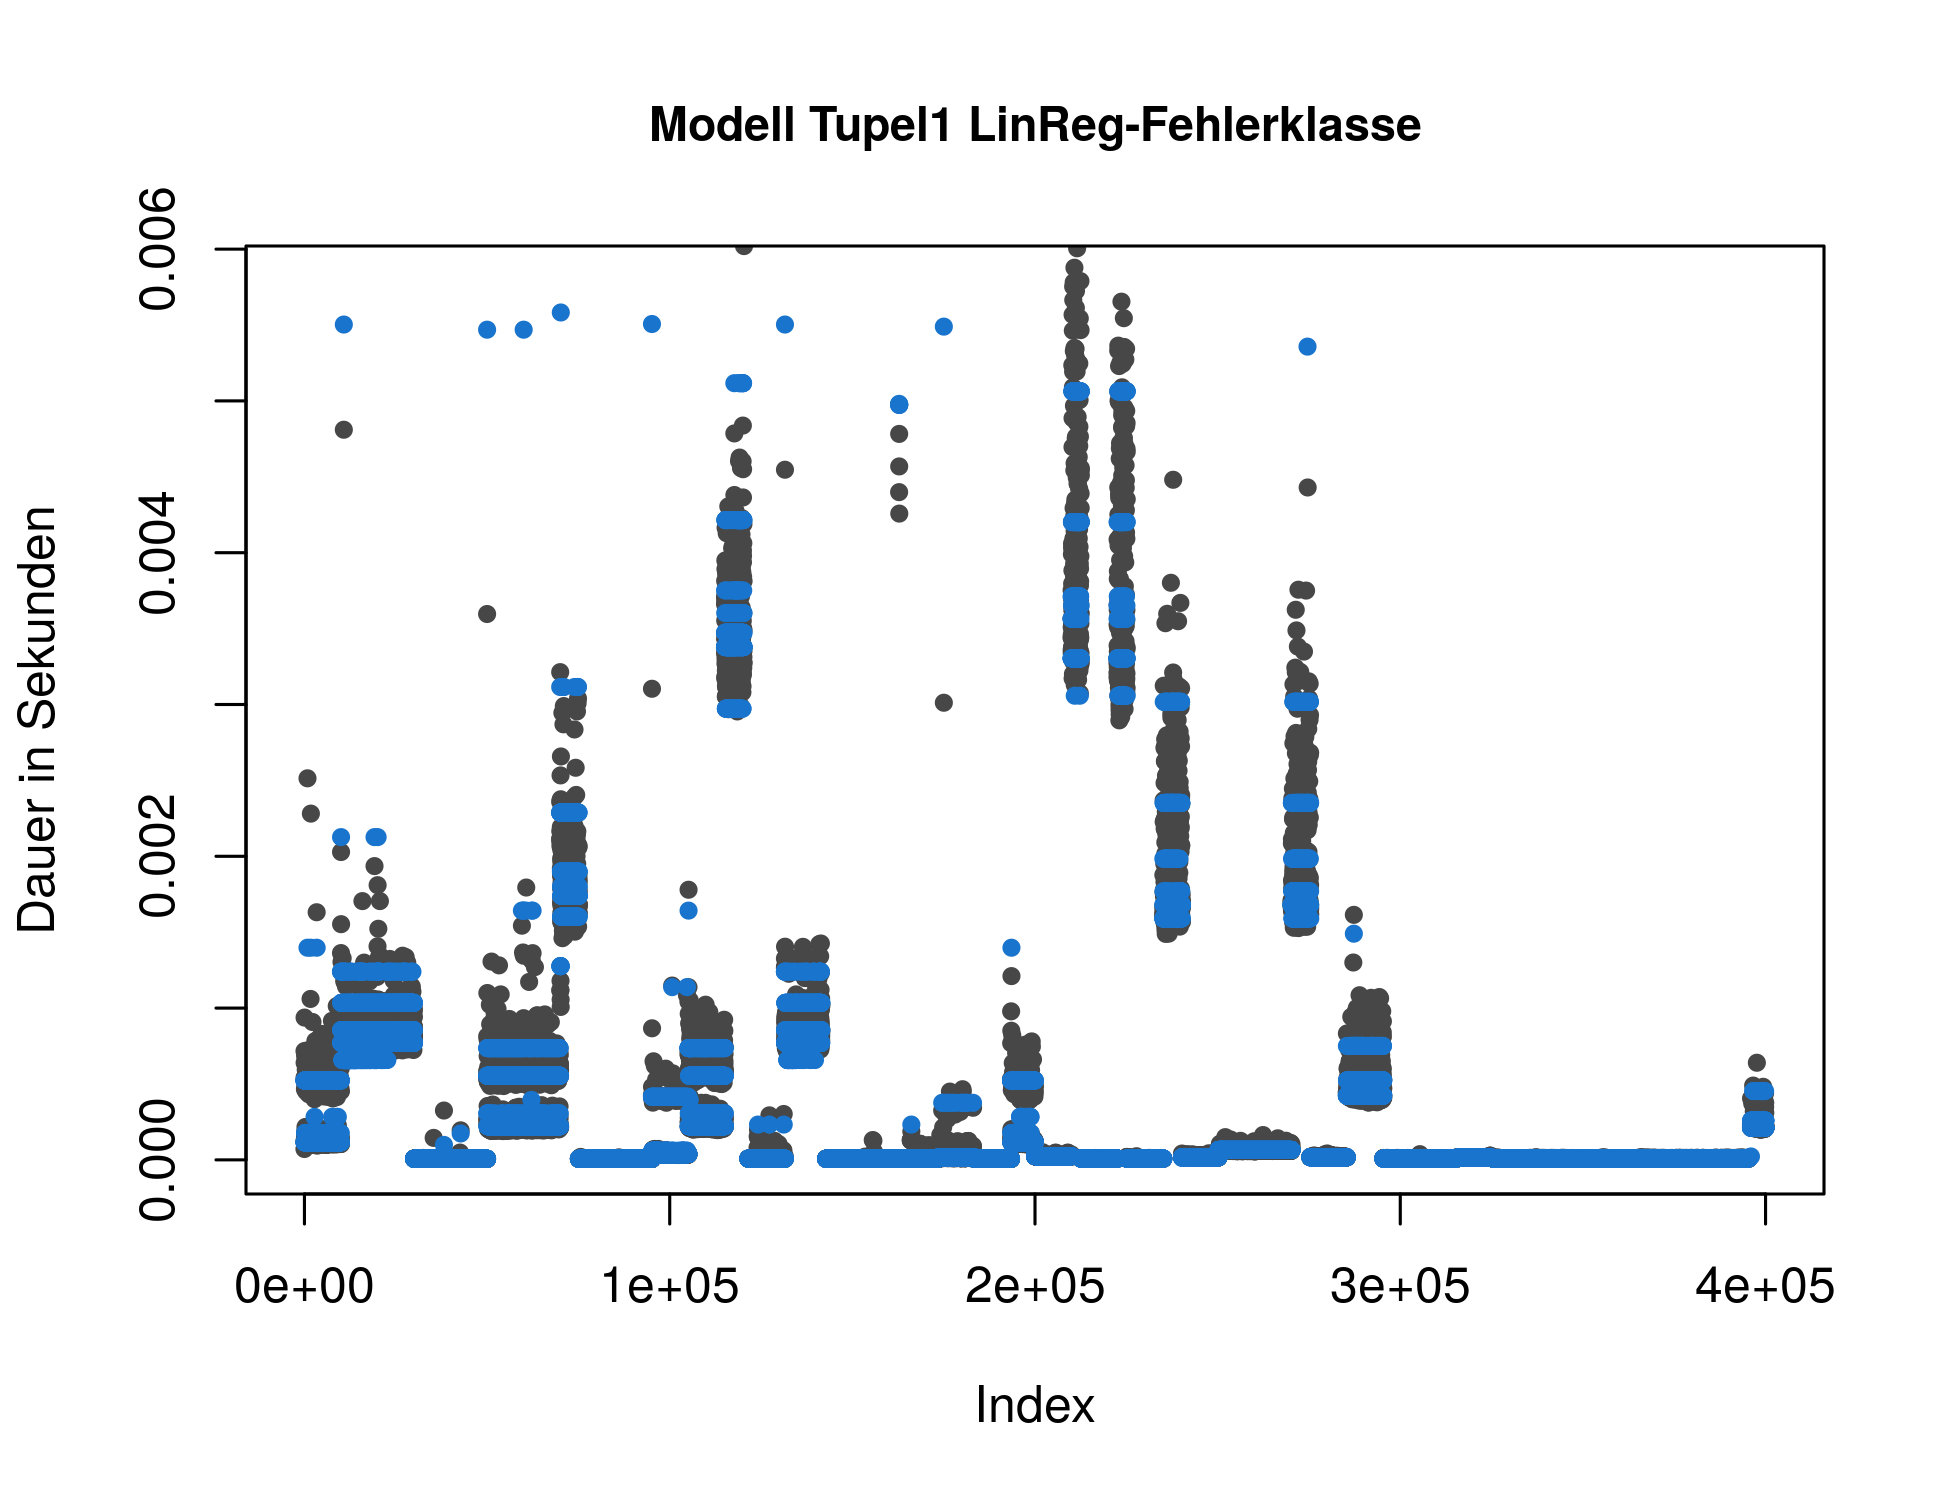
\includegraphics[width=1\linewidth]{Bilder/plot_onlyPred_tuple1_with_error_class_from_linreg_Duration_seq.png}\\
		\vspace*{-0.45cm}
		\caption{NN-LinRegFK auf SEQ}
		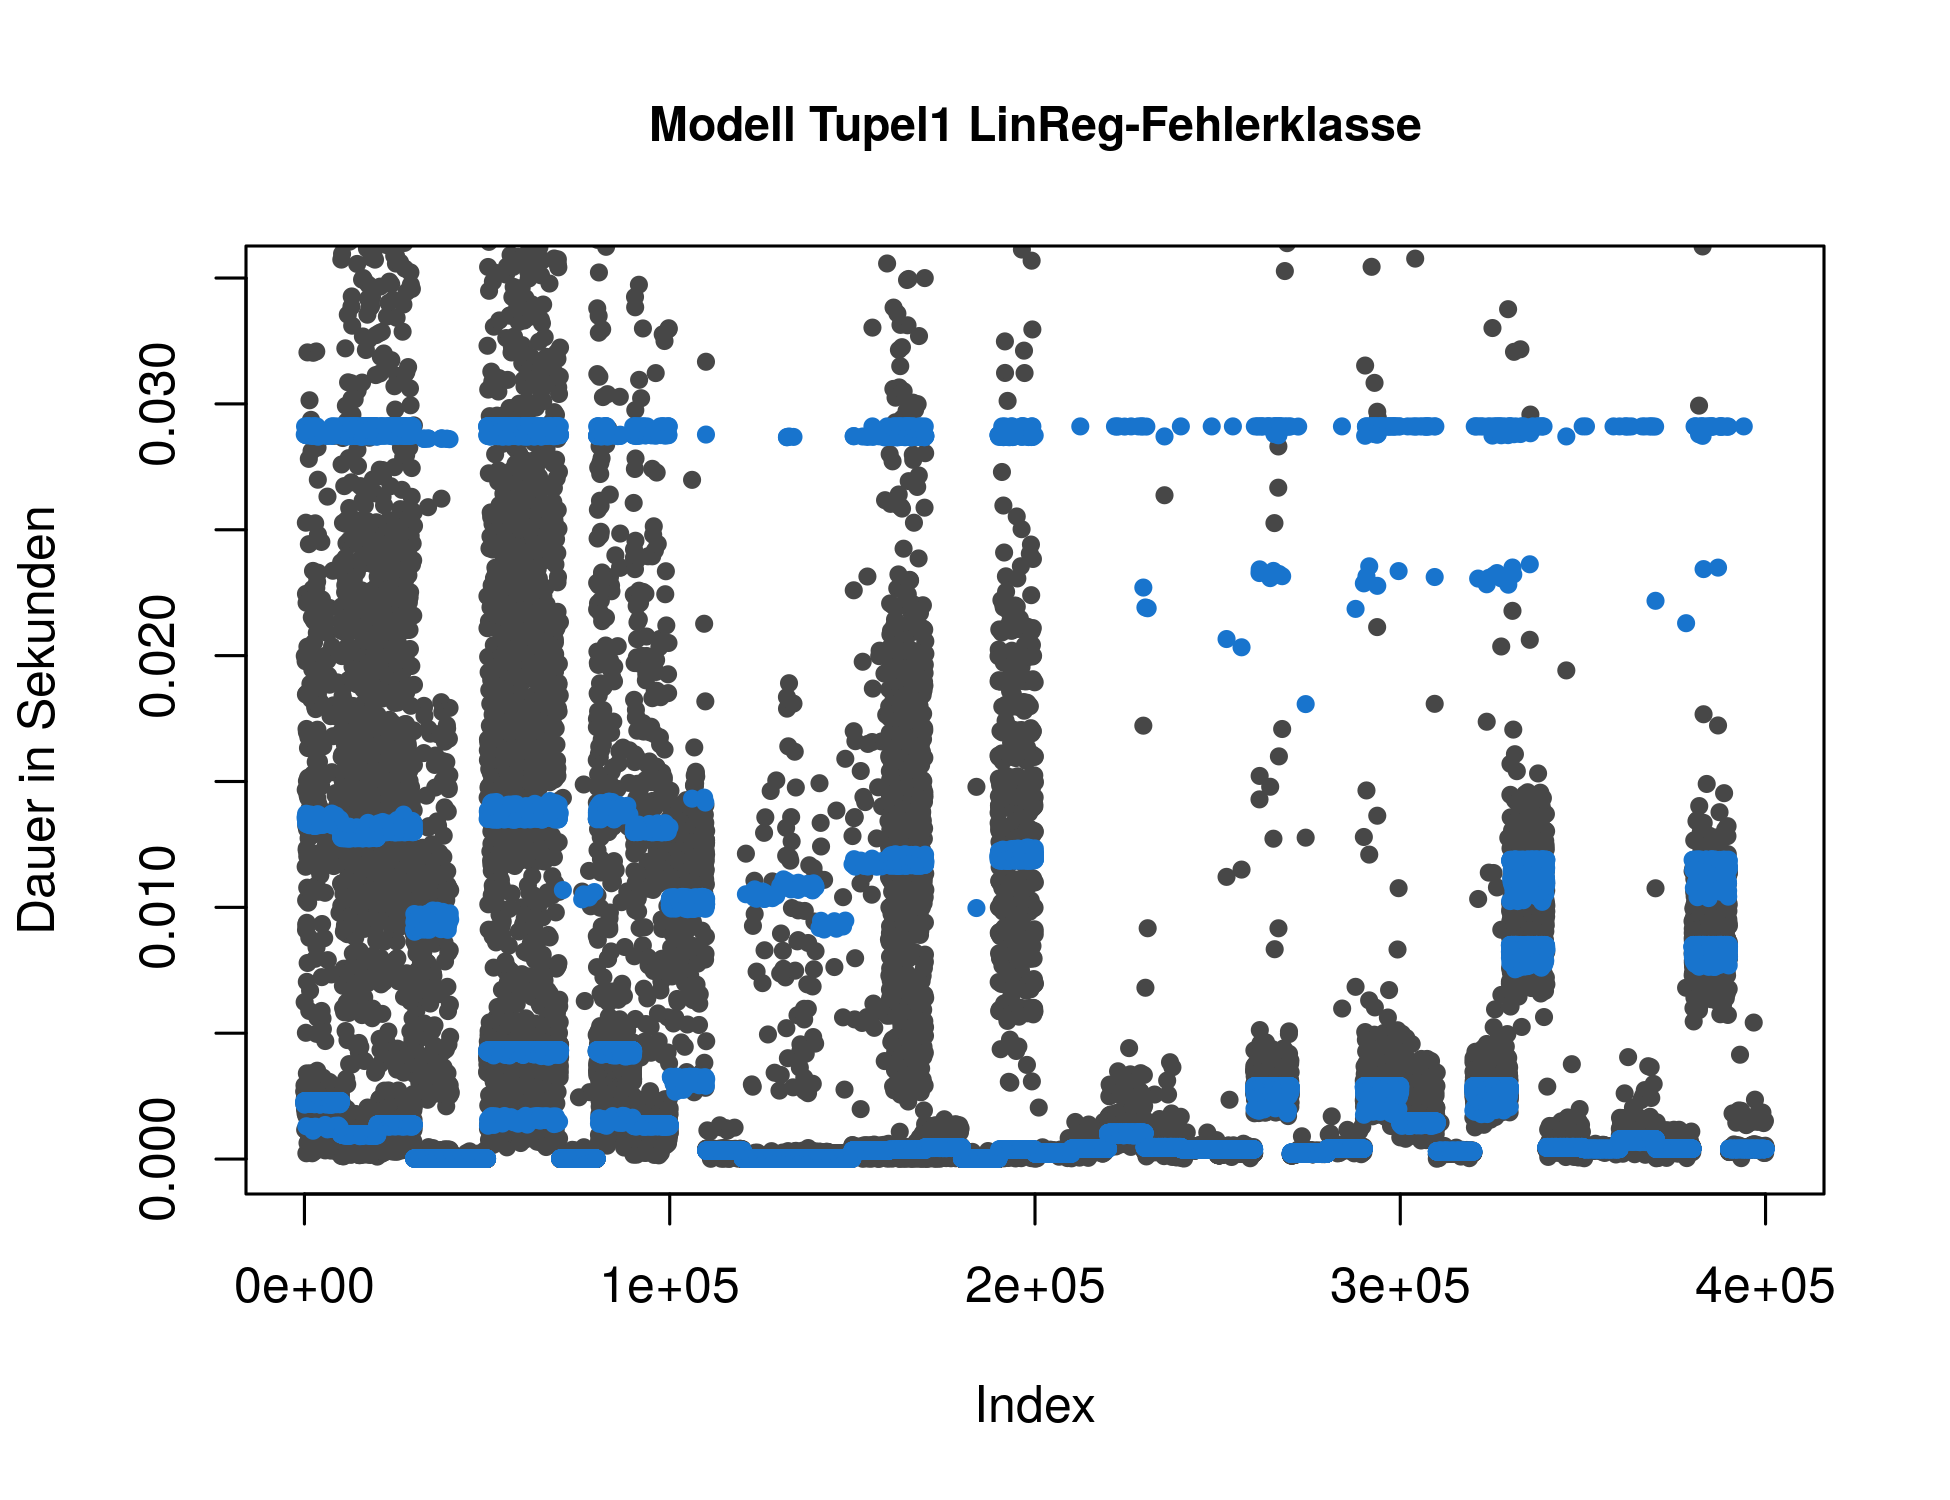
\includegraphics[width=1\linewidth]{Bilder/plot_onlyPred_tuple1_with_error_class_from_linreg_Duration_rnd.png}
		\vspace*{-0.45cm}
		\caption{NN-LinRegFK auf RND}
	\end{figure}
\end{columns}
\end{frame}

\section{Zusammenfassung}
\begin{frame}
\frametitle{Zusammenfassung}
\begin{itemize}
	\item Vorhersagen einfacher Modelle mit neuronalen Netzen teilweise recht gut 
	%13 vs 100 % fehler, bzw. 6µs vs 300µs; im einfachen bzw. schwierigen Fall
	\item Lineare Modelle unzureichend
	\item Entscheidend für eine gute Vorhersage: E/A-Zugriffe mit gleichen Zugriffsparametern unterscheiden können
	\begin{itemize}
		\item Verarbeitung im System kann in E/A-Pfade unterteilt werden
		\item Welcher Pfad genommen wurde ist nicht bekannt
	\end{itemize}
	\item Mit einfachen Modellen, die zeitliche Abhängigkeiten ausnutzen, kann der E/A-Pfad nicht bestimmt werden
	%um eine Näherung der E/A-Pfade zu geben
	%\item Verfahren für die Bestimmung der E/A-Pfade eingeführt
	%\begin{itemize}
	%	\item Clustering der Residuen
	%\end{itemize}
	\item Unterscheidung von E/A-Pfaden durch Fehlerklassen möglich
\end{itemize}	
\end{frame}
%------------------------------------------------
\begin{withoutheadline}
	\begin{frame}
		\Huge{\centerline{Ende der Präsentation}}
	\end{frame}
\end{withoutheadline}

\section*{Reserve Folien}

\subsection*{Exploration der Messdaten}
\frametitle{Detailbetrachtung: 250 Messungen auf RND}
\begin{frame}
\begin{columns}
	\column{.45\textwidth}
	\begin{figure}
		\includegraphics<1->[width=1\linewidth]{Bilder/plot_First250_read_rnd.png}\\
		\vspace*{-0.45cm}
		\caption{RND lesend}
		\includegraphics<1>[width=1\linewidth]{Bilder/plot_First250_write_rnd.png}
		\vspace*{-0.45cm}
		\caption{RND schreibend}
	\end{figure}
	\column{.45\textwidth}
	\begin{figure}
		\includegraphics<1>[width=1\linewidth]{Bilder/plot_From100001to100250_read_rnd.png}
		\\
		\vspace*{-0.45cm}
		\caption{RND lesend}
		\includegraphics<1->[width=1\linewidth]{Bilder/plot_From100001to100250_write_rnd.png}
		\vspace*{-0.45cm}
		\caption{RND schreibend}
	\end{figure}
\end{columns}
\end{frame}

\subsection*{Fehlerklassen}
\begin{frame}
	\frametitle{Fehlerklassen auf SEQ}
	%Klassen sortiert nach durchschnittlichem Residuum!
	%Durchsätze verschiedener Klassen sollten klare Differenzen aufweisen
	%idealerweise verschiedene Klassen für Zugriffe von etwa gleicher Größe
	%Residuen sollten nicht einfach mit der mittleren Zugriffszeit ansteigen / dann hat das Problem den Nutzen kaputt gemacht
	%klare Zuordnung der meisten Messungen in die Klasse mit kleinstem Fehler
	\begin{table}
		\resizebox{\textwidth}{!}{
			\begin{tabular}{|r|r|r|r|r|r|r|r|}\hline%
				& \multicolumn{3}{|c|}{gemittelte Angaben} & \multicolumn{3}{|c|}{Angaben zu den Residuen} & \multicolumn{1}{r|}{zugeordnete Messungen} \\ \hline
				Klasse & Durchsatz (B/s) & Größe (B) & Dauer (s) & Min (s) & Durchschnitt (s) & Max (s) & auf SEQ\\ \hline\hline
				\csvreader[late after line=\\\hline]%
				{CSV/seq_linreg_classes_on_rnd.csv}{tp=\tp,idx = \idx,rndcount=\rndcount,minerror=\minerror, meanerror = \meanerror, maxerror = \maxerror, seqcount = \seqcount, size = \size, duration = \duration}%
				{\idx & \tp & \size & \duration & \minerror & \meanerror & \maxerror & \seqcount}%
			\end{tabular}
		}
	\end{table}
\end{frame}

\begin{frame}
	\frametitle{Fehlerklassen auf RND}
	\begin{table}
		\resizebox{\textwidth}{!}{
			\begin{tabular}{|r|r|r|r|r|r|r|r|}\hline%
				& \multicolumn{3}{|c|}{gemittelte Angaben} & \multicolumn{3}{|c|}{Angaben zu den Residuen} & \multicolumn{1}{r|}{zugeordnete Messungen} \\ \hline
				Klasse & Durchsatz (B/s) & Größe (B) & Dauer (s) & Min (s) & Durchschnitt (s) & Max (s) & auf RND \\\hline\hline
				\csvreader[late after line=\\\hline]%
				{CSV/rnd_linreg_classes_on_seq.csv}{tp=\tp,idx = \idx,rndcount=\rndcount,minerror=\minerror, meanerror = \meanerror, maxerror = \maxerror, size = \size, duration = \duration}%
				{\idx & \tp & \size & \duration & \minerror & \meanerror & \maxerror & \rndcount}%
			\end{tabular}
		}
	\end{table}
\end{frame}

\subsection*{Ausblick}
\begin{frame}
	\frametitle{Ausblick}
	\begin{itemize}
		\item Periodische Zusammenhänge im E/A-System besser ausnutzen
		%für einzelne Festplatten ist dies sehr erfolgreich
		\item Zusammenhang zwischen Fehlerklassen und E/A-Pfaden genauer untersuchen
		\item Fehlerklassen aus Residuen verschiedener Modelle vergleichen
		\item Problem beheben, dass die Residuen größerer Laufzeiten die Fehlerklassen dominieren
	\end{itemize}	
\end{frame}
%----------------------------------------------------------------------------------------

\end{document} 